\documentclass[12pt, a4paper]{article}
\setcounter{tocdepth}{2}
\usepackage{graphicx} % Required for inserting images
\usepackage[parfill]{parskip} % Removes indent from new paragraphs
\usepackage{amsmath, amssymb, amsfonts}
\usepackage[colorlinks = true,
			citecolor  = blue,
            linkcolor = black]{hyperref}
\usepackage[font={scriptsize}]{caption} % Figure caption font
\usepackage[labelfont=bf]{caption} % Bold figure x.x 
\captionsetup{width=0.9\textwidth}
\usepackage{algorithm}
\usepackage{algpseudocode}

\usepackage[natbibapa]{apacite}
\bibliographystyle{apacite}
% \usepackage[longnamesfirst,authoryear, round]{natbib}
% \bibliographystyle{unsrtnat}
\usepackage{float}
\usepackage[
top    = 1.0in,
bottom = 1.2in,
left   = 1.0in,
right  = 1.0in]{geometry}
\linespread{1.5}

\title{Comparing MCMC algorithms for Stochastic Volatility Model Bayesian Posteriors using Simulation Based Calibration}
\author{Benjamin Wee}
\date{October 2023}

\begin{document}

\maketitle 

\begin{abstract}
    This research compares the computational methods used to estimate Bayesian stochastic volatility models. The MCMC approaches outlined in the stochastic volatility literature and Hamiltonian Monte Carlo are assessed in their ability to sample from the model's posterior distribution. Specifically, Simulation Based Calibration (SBC) is used to check whether these MCMC algorithms are returning efficient and calibrated posterior estimates. Key metrics of interest are the effective sample size to check the efficiency of the algorithm and tests of uniformity to assess the calibration of the posteriors. This will determine which method is better at estimating stochastic volatility models based on the efficiency and accuracy of the sampling strategy. Results reveal that Hamiltonian Monte Carlo provides more efficient and calibrated posterior estimates of the stochastic volatility model conditional on model parameterisation. 
\end{abstract}

\newpage

\tableofcontents{\protect\newpage}

\section{Introduction}
    Stochastic volatility (SV) models are used in financial econometrics to model and predict the behaviour of financial asset returns. Typically expressed as a non-Gaussian state space model where the conditional variance of the observed return is treated as a latent random variable \citep{hull1987pricing, chesney1989pricing}, such models are difficult to estimate since the likelihood is unavailable in closed form. With more parameters than observations,\footnote{We refer to both static unknowns and time-varying latent state variables as 'parameters'.} SV models are commonly analysed using Bayesian methods obtained via a Markov Chain Monte Carlo (MCMC) algorithm designed to sample from the high dimensional joint posterior distribution. The focus of this paper is to investigate the performance of two competing MCMC algorithms, each applied to a SV model, in terms of the validity and statistical efficiency of the their resulting inference. Performance of these algorithms will also be compared with different parameterisations of the SV model to determine the sensitivity of each MCMC to model specification.

    \citet{kim1998stochastic} propose a sampling strategy for the so-called 'vanilla' stochastic volatility through an off-set mixture approximation. Conditional on the mixture allocations and static parameters, the forward filter backward sampling algorithm (Carter and Kohn, 1995; Fr{\"u}wirth-Schnatter, 1995) is used to jointly sample the latent states while conditionally  conjugate prior distributions are also suggested.  Since then, there have been many advances in statistical computing and algorithm design. In particular, Hamiltonian Monte Carlo (HMC) has be proposed as a generic and efficient sampling method for MCMC. Notably, HMC has been shown to be particularly well-suited to complex, high dimensional probabilistic models. Importantly, the adoption of such new techniques have been made widely available through the development of various open source libraries such as the Stan programming language \citep{stan} and the PyMC library \citep{pymc2023}. As the development of new algorithms rapidly increase, so does the need to develop new methods to assess their output. Developments in statistical workflow are required to test new algorithms as well as compare computational strategies used to estimate increasingly complex models.

    This research analyses and compares the calibration and efficiency of MCMC used to estimate stochastic volatility models using a simulation study. By calibration we refer to a MCMC algorithm that returns correct posterior, on average, conditional on the correct model specification. The first algorithm replicates Kim Shephard and Chib's (KSC) Gaussian mixture approximation which is sampled using the aforementioned Kalman Filter and Metropolis Hastings algorithm. The second algorithm is the No-U-turn sampler (NUTS) variant of Hamiltonian Monte Carlo (HMC) as implemented in the Stan programming language \citep{hoffman2014no, betancourt2017conceptual, stan}. The objective is to analyse the efficiency of the MCMC and their ability to return correct posterior estimates.

    Comparisons of these algorithms are conducted using a methodology known as Simulation Based Calibration (SBC) \citep{talts2018validating}. Parameters are drawn from the prior distribution and used to create data sets from the generative stochastic volatility model. We then obtain posterior samples from each of the MCMC methods. Repeating this process multiple times gives insight to how well the MCMC algorithm can estimate the true parameters given the data generating process. The key diagnostic metrics are the effective sample size, to measure the efficiency of the algorithm, and uniform rank statistics to determine calibration of the posterior estimates. 

    One particular challenge to comparing models is the parameterisation. Different parameterisations of a model, whilst the same mathematically, can be very different in terms of sampling difficulty \citep{neal2003slice}. In this work two different parameterisations of the stochastic volatility model are compared for each sampling method. An algorithm may be sensitive to different parameterisations of the same model which may impact MCMC performance as described in \citet{strickland2008parameterisation}. The key findings of this research are HMC applied on a re-parameterised SV model produces the most calibrated and efficient posterior estimates and that the MCMC algorithms may perform better or worse based on calibration and efficiency depending on the parameterisation of the model.

    This paper is structured as follows. Section 2 provides the context around this research through the introduction of the stochastic volatility model and a discussion of the limitations of using ad-hoc simulations and MCMC convergence diagnostics to determine posterior calibration (or validity). Section 3 describes the SBC methodology, along with the simulation design and diagnostic metrics used for the SV model. Section 4 details key aspects of the two MCMC sampling approaches under consideration, while Section 5 discusses the results and limitations. Finally, Section 6 concludes and provides points for further research.

\section{Research Context}

\subsection{Stochastic Volatility}
    The model of interest is the discrete time, uni-variate stochastic volatility model estimated by \citet{kim1998stochastic} using Bayesian framework. SV is expressed as a state space model which links the observed mean corrected (logarithmic) return of a given asset to the latent conditional variance. 
    \begin{align}
    y_t =& \space \exp(h_t/2) \varepsilon_t, \\
    h_{t+1} =& \space \mu +\phi(h_t - \mu) + \sigma_{\eta} \eta_t,  \\
    h_1 \sim& \space \,\mathrm{N}\left(\mu, \frac{\sigma_{\eta}^2}{1-\phi^2}\right), \\
    \varepsilon_t \sim& \space \,\mathrm{N}(0,1), \\
    \eta_t \sim& \space \,\mathrm{N}(0,1).
    \end{align}
    $y_t$ is the mean corrected (logarithmic) return of a given asset, observed over an interval with fixed length and associated with period t. The measurement equation (1) describes the conditional distribution of $y_t$ given $h_t$, where $h_t$ is the conditional log variance of $y_t$. $h_1$ is a draw from a stationary distribution and the state equation $h_{t+1}$ follows a stationary process governed by the auto-regressive parameter $\phi$ such that $|\phi|<1$. This auto-regressive parameter represents the persistence or stickiness of log volatility and the dispersion parameter $\sigma_{\eta}$ is the constant variance of the states. $\epsilon_t$ and $\eta_t$ are standard normal white noise shocks and are uncorrelated with each other.

    KSC assign certain independent prior distributions and hyperparameters to the static parameters, with conjugate priors for $\mu$ and $\sigma^2$, given by
    \begin{align}
    \mu \sim& \space \,\mathrm{N}(0, 10^2) \\
    \sigma_{\eta}^2 \sim& \space \, \mathrm{IG}(shape=5/2, scale=(0.01\times 5) / 2) \\
    \phi^{\ast} \sim& \space \,\mathrm{Beta}(20, 1.5) \\
    \phi =&  2\phi^{\ast} - 1
    \end{align}
    The prior distribution for $\phi$ is referred to as a stretched beta distribution, as it corresponds to a transformed beta random variable, $\phi^*$, with support (-1, 1).
    


\subsection{Challenge 1: Comparing posteriors with no ground truth}
    The stochastic volatility model can be estimated using a variety of sampling strategies and MCMC algorithms. Convergence metrics assessed from the same MCMC output to be used for posterior inference are commonly used to check the performance of the MCMC chains. Most often, the effective sample for each parameter is produced, as it indicates the number of approximately independent draws obtained from the dependent Markov chain for a target parameter \citep{gelman2013bayesian}, and $\hat{R}$, the potential scale reduction factor or measure of variability between different chains \citep{gelman1992inference}, is computed, to gauge whether the MCMC algorithm has converged to the target posterior distribution.

    Convergence diagnostics are useful for identifying when Bayesian computation fail on real data. However, confounding issues may arise when attempting to diagnose the cause of computational problems. Real data is generated from an unknown data generating process. That is, the true parameter and model are unobservable, and it is very likely that the model being fit is not the true model. Therefore, failed diagnostic checks could be the result of attempting to fit a misspecified model, issues with the MCMC algorithm, or both. Furthermore, different sampling strategies will result in different posterior estimates for the same model. Assuming no issues with the computation or the model specification, convergence diagnostics do not provide any guidance to the analyst regarding which posterior estimate is to be preferred since there is no ground truth.

    To illustrate the concerning issues, the posterior distribution associated with the stochastic volatility model in (1)-(5) and a set of real financial returns is estimated using two different MCMC algorithms. The data are demeaned daily (logarithmic) returns on the S\&P 500 Index over the period from 1 January 2023 - 10 September 2023 with sample size $T=171$. Figure \ref{fig:realdataex} displays the marginal posterior estimates for the static parameters $\mu$, $\phi$ and $\sigma^2$, with corresponding summary statistics in Table \ref{tab:realdata}. Overall the two methods are similar in skew and shape. However, closer inspections suggests that $\phi$ has a fatter left tail for the KSC sampler and $\sigma^2$ is also heavier in the right tails relative to HMC. This is evident in the quantiles with the 25th quantile for $\phi$ being smaller at 0.875 for KSC compared to 0.910 in HMC. Furthermore, HMC has taller peaks at their mode relative to KSC with a tighter spread. The uncertainty intervals created from each posterior sample would also be quite different and lead to different results. However, we can only conclude that there are differences between these methods, not which is correct.
    
    % Other methods for model selection in this context (for example, out of sample predictive performance), but for parameter estimation it is unclear which one should be selected. 

    \begin{figure}[H]
        \centering
        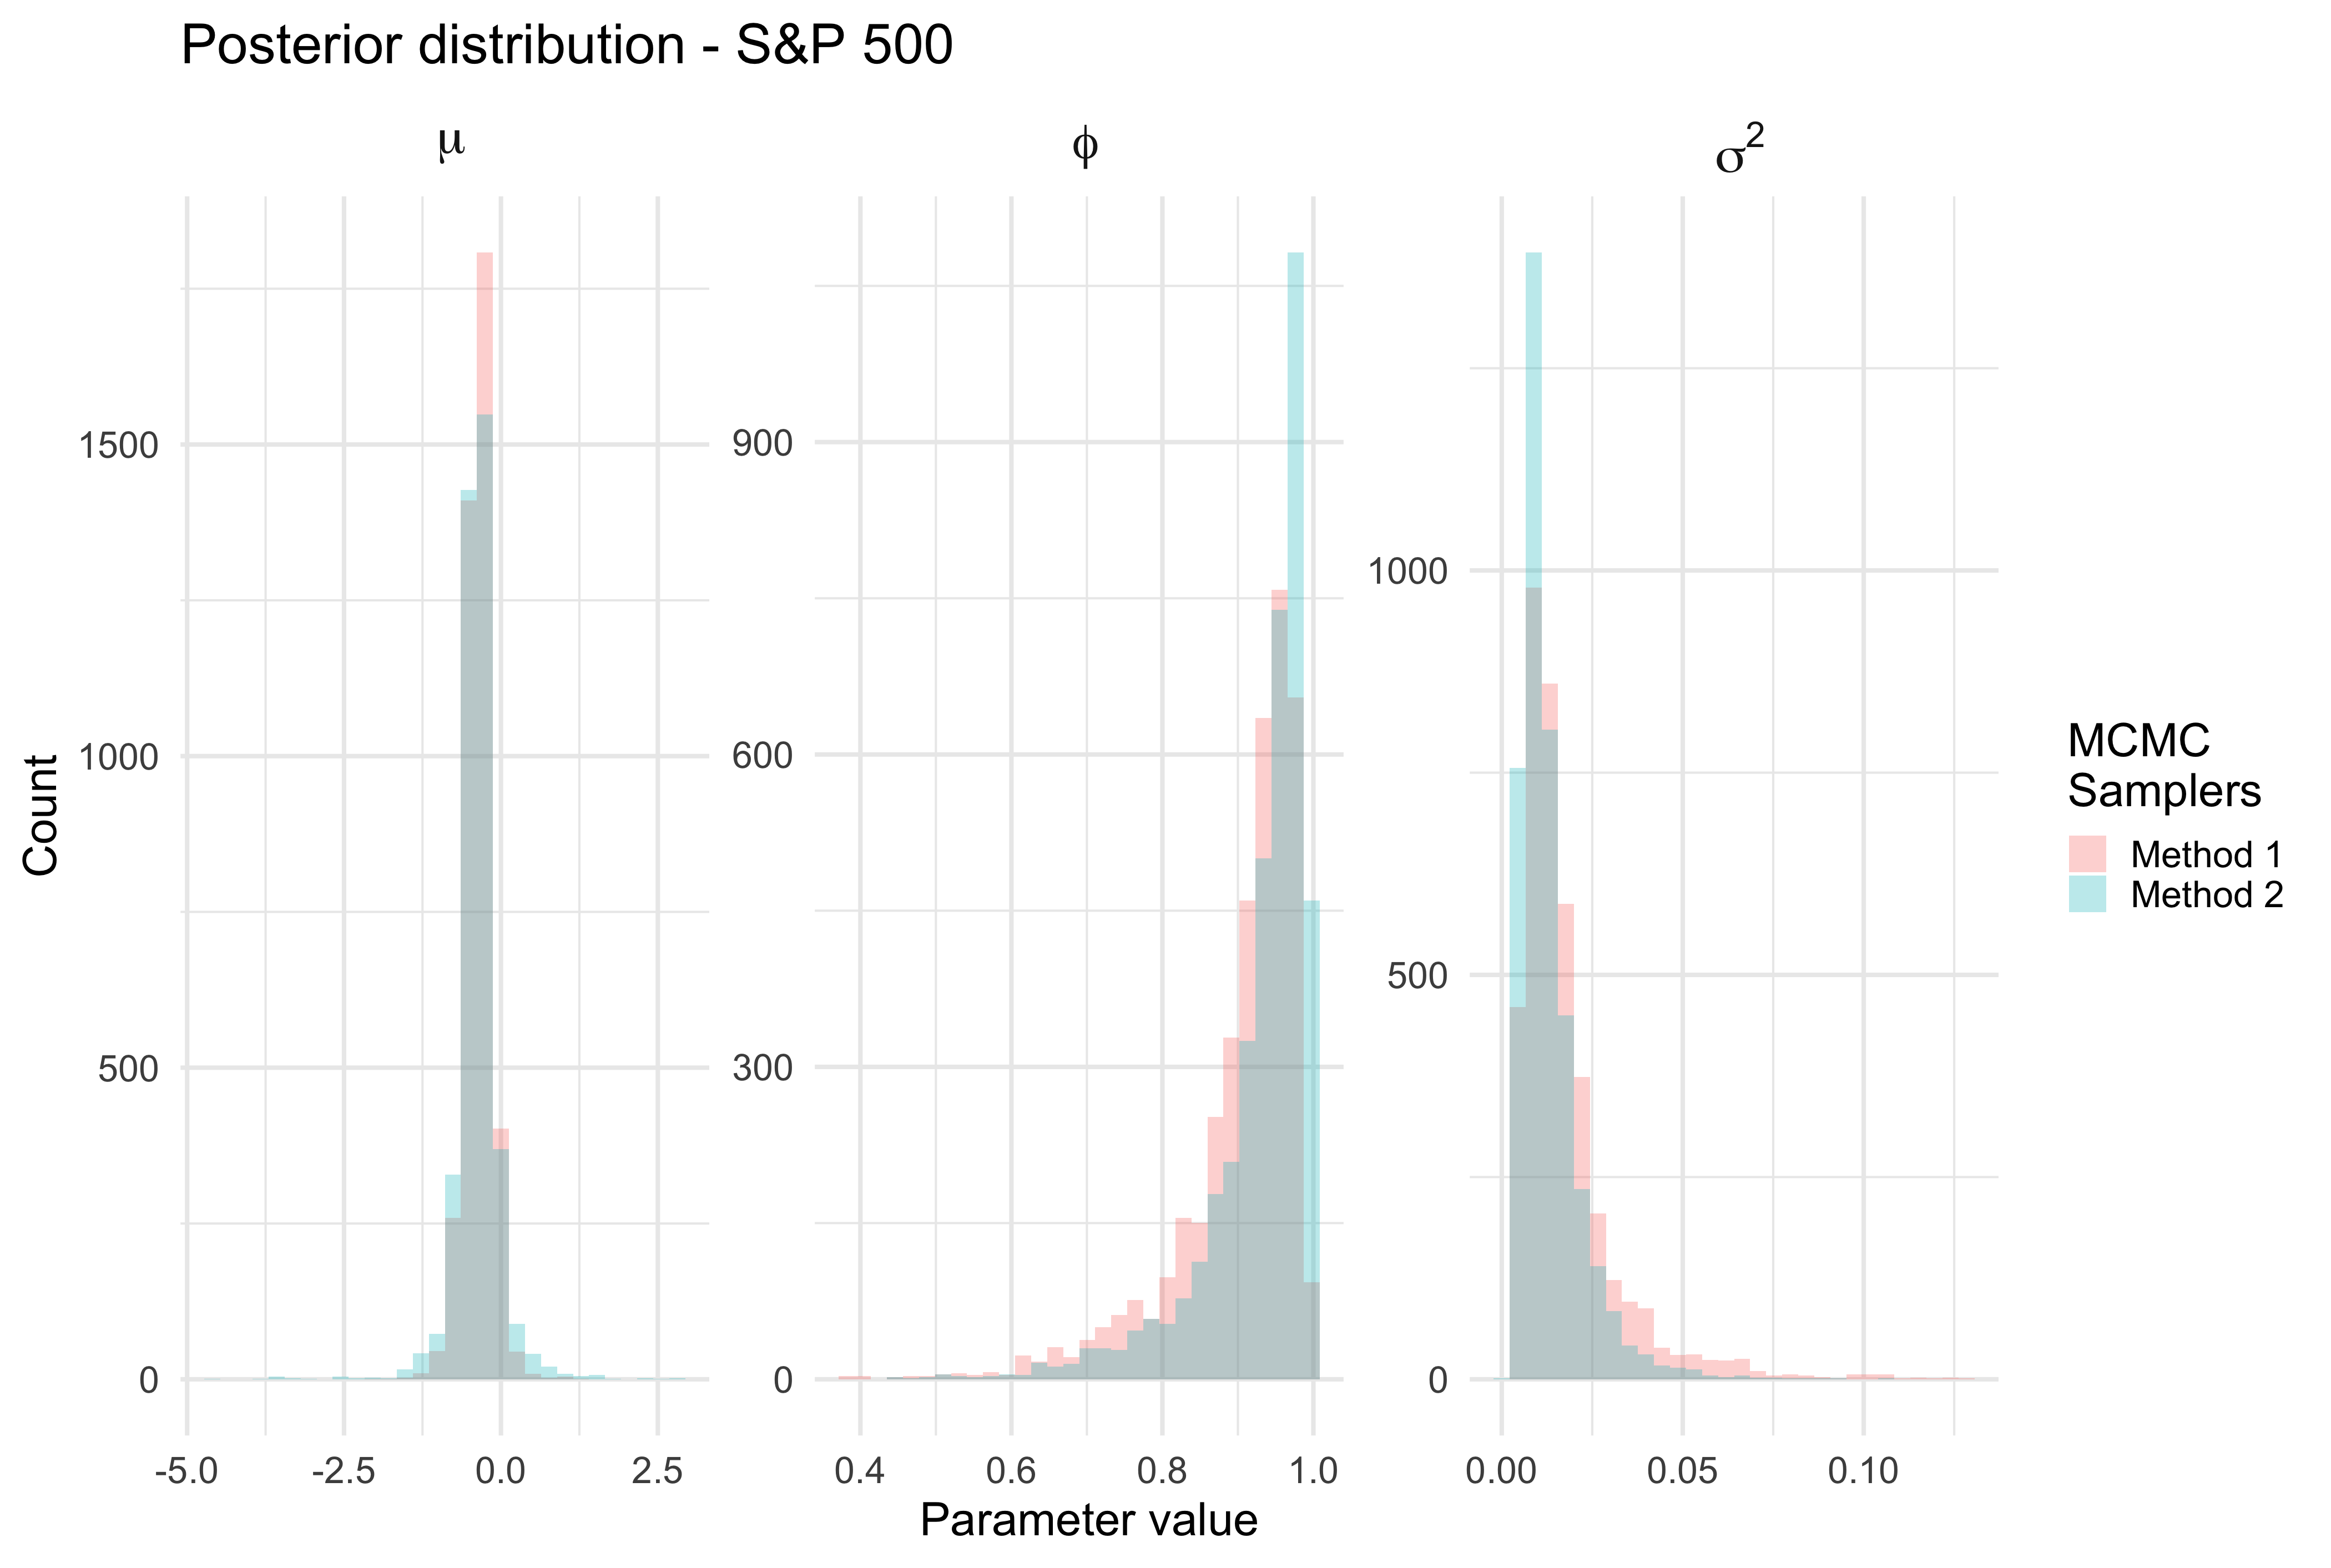
\includegraphics[scale=0.1]{motivating_example/real_data_ex.png}
        \caption{\textbf{Posterior distribution for static parameters fit on the S\&P 500 Index.} Posterior samples from the HMC (blue) and KSC (red) MCMC samplers.}
        \label{fig:realdataex}
    \end{figure}

    \begin{table}[H]
        \centering
        \begin{tabular}{|c|c|c|c|c|c|c|c|} \hline 
        Parameter&  MCMC&Min& q25&  Median& Mean & q75&Max\\ \hline 
        $\mu$&  KSC&-2.03 & -0.472 & -0.354 & -0.355 & -0.231 & 1.31 \\
     $\mu$&  HMC&-4.55 & -0.508 & -0.373 & -0.370 & -0.229 &2.86  \\\hline 
     $\phi$&  KSC&0.384 & 0.875 & 0.928 & 0.902 & 0.958 & 0.997 \\
     $\phi$&  HMC&0.438 & 0.910 & 0.953 & 0.929 & 0.977 &1.00  \\ \hline 
     $\sigma^2$&  KSC&0.00237 & 0.00891 & 0.0138 & 0.0178 & 0.0210 & 0.130 \\ 
     $\sigma^2$&  HMC&0.00209 & 0.00731 & 0.0105 & 0.0131 & 0.0159 &0.107 \\ \hline
        \end{tabular}
        \caption{\textbf{Summary statistics for HMC and KSC algorithms}. Both sets of estimates appear reasonable but it is unclear from estimates on real data which estimate is closer the the truth.}
        \label{tab:realdata}
    \end{table}
    
\subsection{Challenge 2: Limitations of a single simulation}
    Diagnosing problems with the approximate posterior from models fit to real data is difficult because we do not have a ground truth to compare with. A strategy around this is to evaluate a model and algorithm on simulated data. One approach is to simulate data from a generative model using known parameters. Then fit the same model on the simulated data and see if the true parameters can be recovered. This gives us the benefit of defining the true parameters of the data generating process to be estimated. If the model and algorithm cannot adequately capture the true parameter, then we cannot be confident that it will provide reliable estimates on real data.

    Simulation is particularly important in the SV model as it has latent parameters. \citet{gelman2020bayesian} discuss that simulation is the only way we can check inference on latent variables. This is critical for the SV model since the underlying framework is a state space model with latent log volatility parameters. Latent variables are unobserved in real data and are only estimated in the context of the model. Simulation gives control over the data generating process which reveals what the model can infer about the latent variables. 

    Simulations enable the analyst to check whether a model and corresponding simulation algorithms appropriately estimate the `true' data generating process. However, there are limitations to what can be learned from a single simulation. Even for a correctly specified model, there is always a small probability that the true parameter is in the tails of the corresponding (exact) marginal posterior distribution. \cite{talts2018validating} make the point that a single simulation does not provide sufficient information about the inference made by an algorithm. As discussed in their paper, a single simulation may conclude ``that an incorrectly coded analysis worked as desired, while a correctly coded analysis failed''. 

    Figure 2 shows marginal posterior distributions given a single set of 1000 returns generated by the SV model. The true parameters are $\mu=-0.389$, $\sigma^2_{\nu}=0.0115$ and $\phi=0.547$ and the model is fit using Stan's implementation of HMC, the No-U-Turn sampler. The 95\% credible intervals for $\mu$ and $\sigma^2$ cover the true parameter. The true parameter for $\phi$ however, is in the tails and outside the interval. Such an analysis may incorrectly conclude that the model fails to adequately estimate the $\phi$ parameter. However, it may be the case that the posterior distribution is correctly calculated using this algorithm and the results may be due to the features of this specific simulated data set.

    \begin{figure}[h]
        \centering
        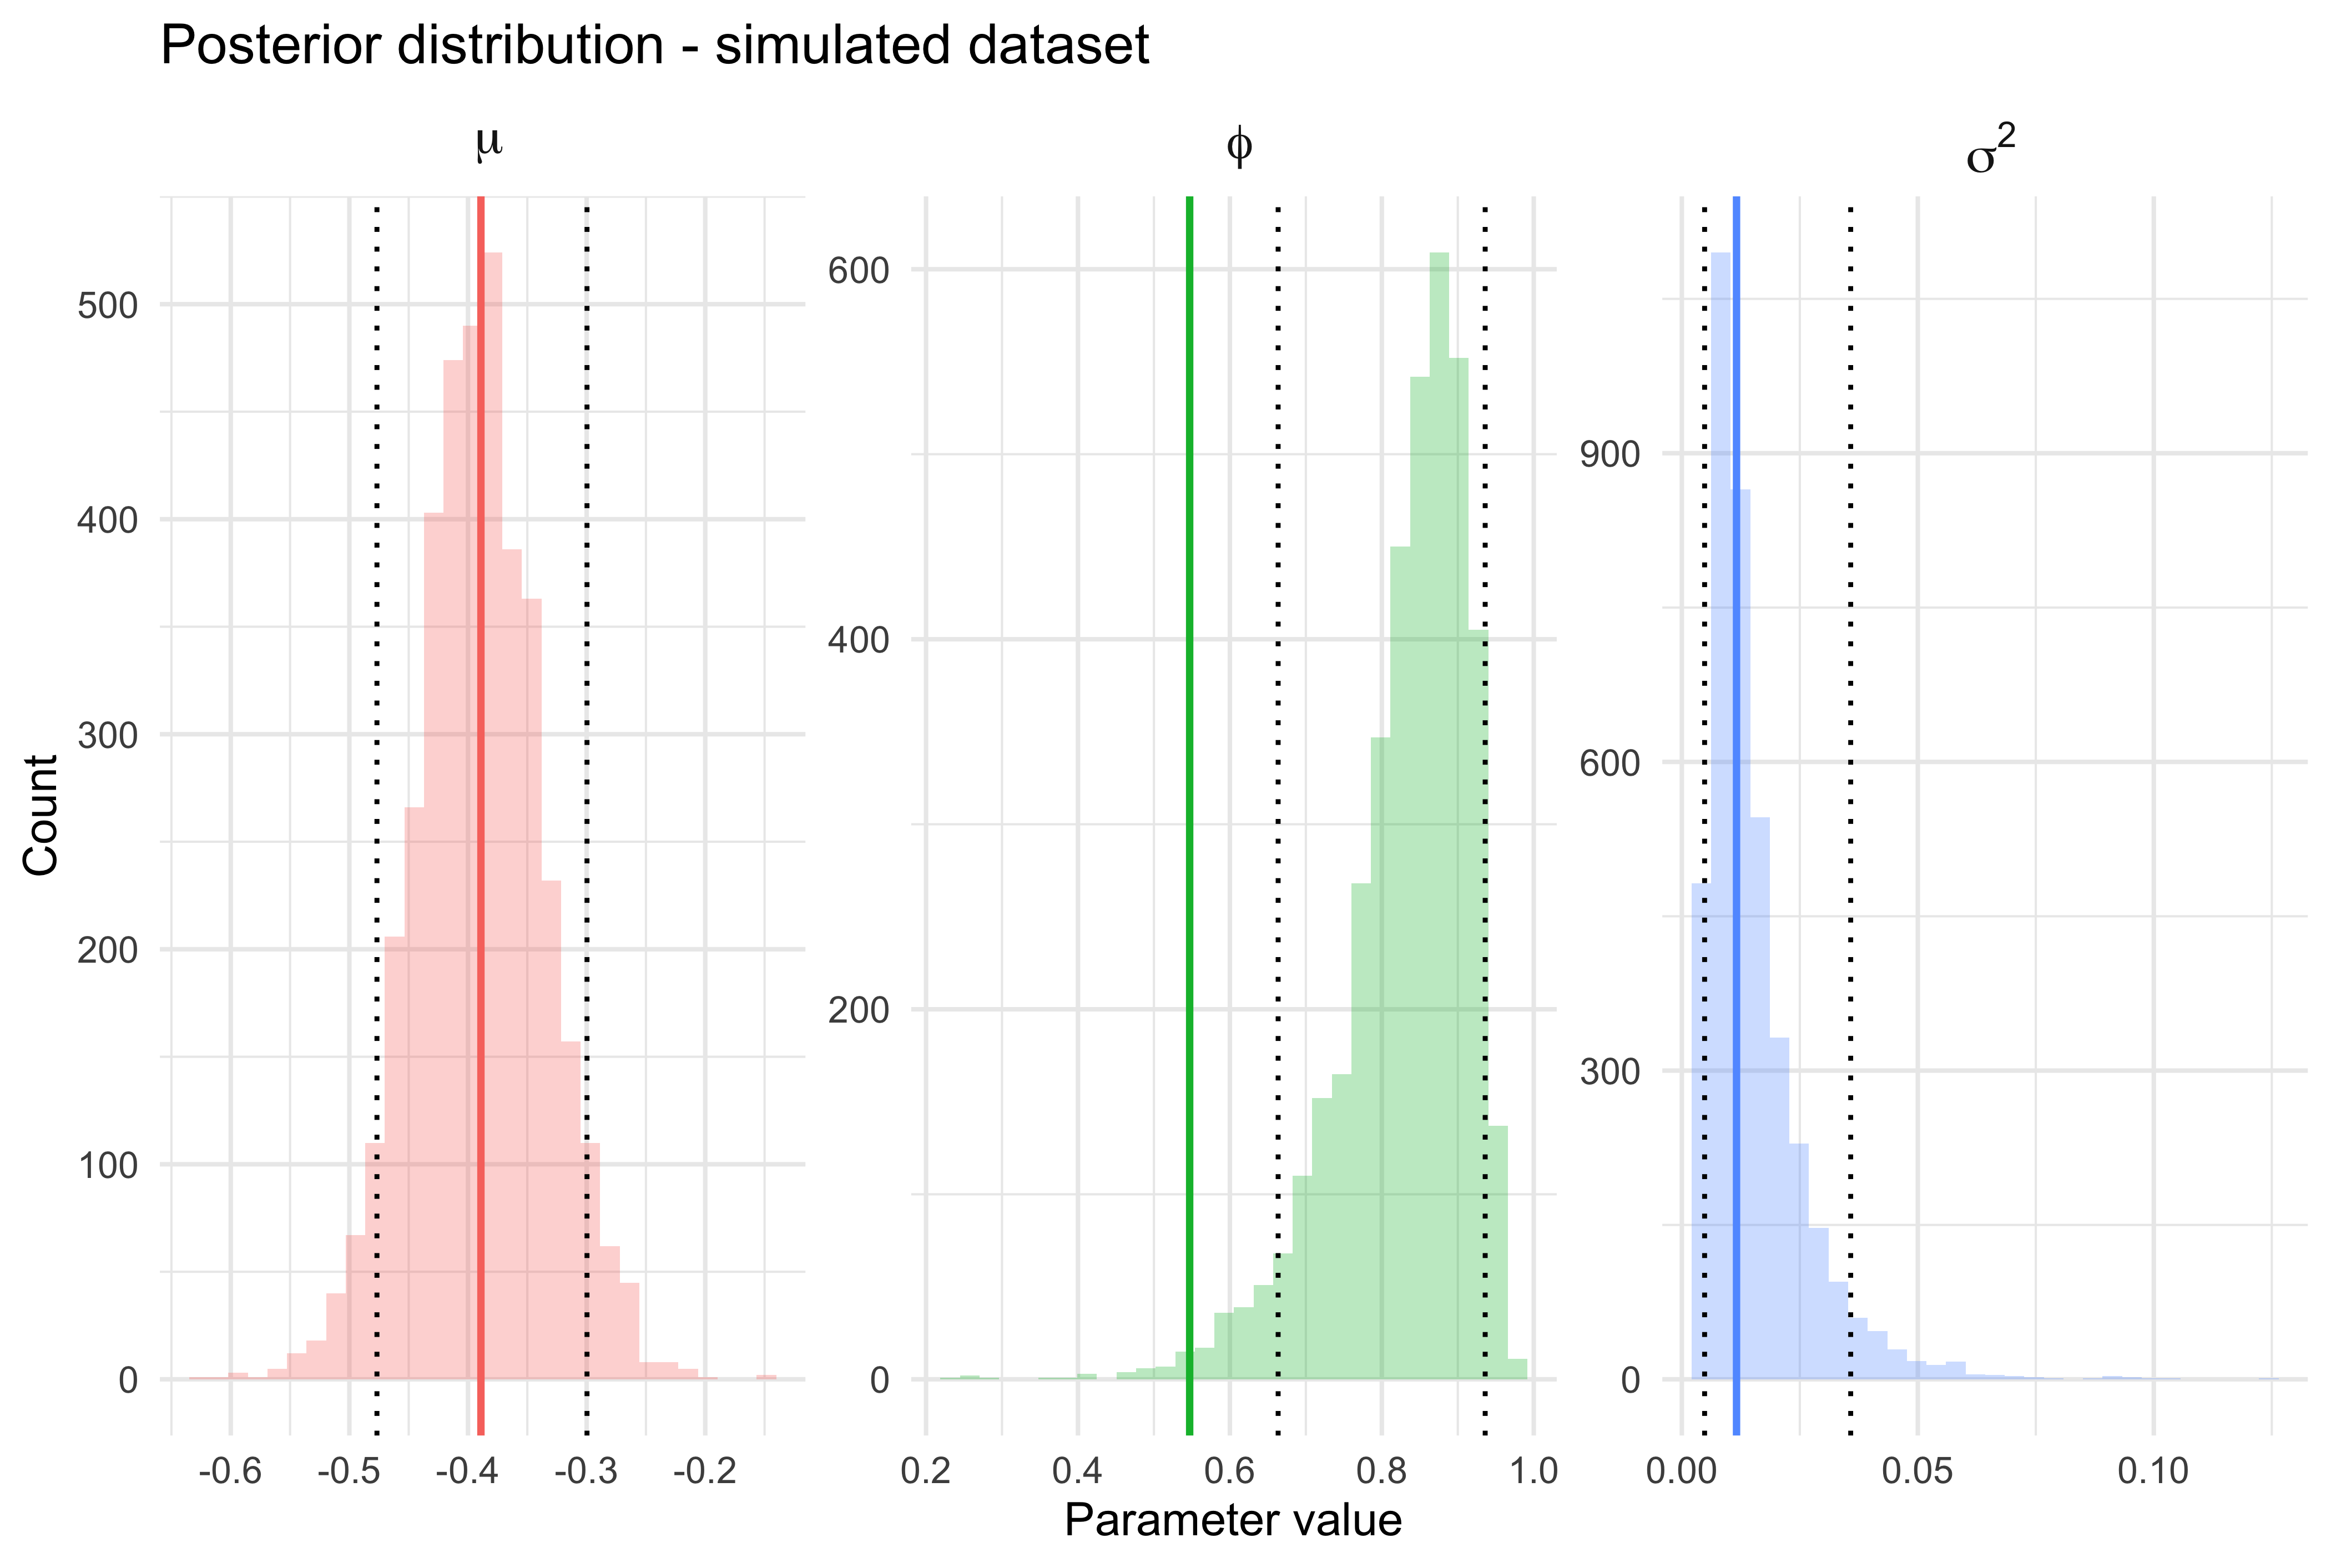
\includegraphics[scale=0.1]{motivating_example/single_sim.png}
        \caption{\textbf{Posterior samples from SV model fit on known data generating process}. Vertical solid line represents true parameter and dotted lines are 95\% credible intervals around the mean. The parameter $\phi$ falls outside the credible interval whereas $\mu$ and $\sigma^2$ stay inside.}
    \end{figure}

\subsection{Research Goal}
    The objective of this research is to design a simulation study to evaluate the calibration of the HMC and KSC offset-mixture algorithms used to estimate SV models. As discussed, there are limitations to evaluating MCMC algorithms based on fits to real data and single simulations. To check the calibration of an algorithm, repeated independent simulations are required. This methodology is discussed in the next section. 

    Two parameterisations of the SV model for each sampler will be implemented using this simulation design. Results from the study will also be used to compare both sampling strategies to determine which MCMC approach is most suitable for estimating this model. 

\section{Methodology}

    \subsection{Simulation Design}
        Simulation Based Calibration (SBC) checks the calibration of posterior estimates generated by MCMC algorithms. SBC is conducted by comparing the distribution of rank statistics to the uniform distribution which arises when an algorithm is correctly calibrated. For each $k$ of $K$ SBC iterations, one value for each parameter is drawn from the prior. For this parameter a data set is generated from the model. Then a sampling method (originally using Stan in \citet{talts2018validating}) is used to obtain posterior samples given this data and the prior. Then the estimated posteriors are compared to the true values by calculating the rank. Under a calibrated model, the $K$ rank statistics for each parameter should be uniformly distributed. 

        To illustrate the SBC procedure, let $\theta$ be an arbitrary scalar parameter from a model and $y$ represent a data set. Start with a single parameter $\theta^{sim}$ drawn from the prior distribution:
        \begin{align}
        \theta^{sim} \sim \pi(\theta),
        \end{align}
        generate a data set $y^{sim}$ conditionally given $\theta^{sim}$ and the model of interest\footnote{Since all computation presumes a correctly specified model, nottation to condition on the model is suppressed.}:
        \begin{align}
        y^{sim} \sim \pi (y|\theta^{sim}).
        \end{align}
        Then take $L$ draws from the estimated posterior distribution, conditional on this data set, and generated by the MCMC algorithm under investigation (here, HMC or KSC):
        \begin{align}
        \{\theta_1,\dots , \theta_{B}\} \sim \pi (\theta | y^{sim}).
        \end{align}

        \citet{talts2018validating} prove that the sample of rank statistics for a given parameter, produced from replicate posteriors, follow a uniform distribution if the posterior samples follow the same distribution as the prior on average. The rank statistic for $\theta$ produced by the $k^{\mathrm{th}}$ replicate posterior sample, is defined as
        \begin{align}
        r^{(k)} = rank(\{\theta_1^{(k)},\dots , \theta_{L}^{(k)}\}, \theta^{sim}) = \sum_{b=1}^{B}1[\theta_{b}^{(k)} < \theta^{sim}].
        \end{align}

        This completes one iteration of SBC. To complete the algorithm, multiple iterations are run and the rank statistics are calculated for each parameter. The resulting rank statistics are compared to the uniform distribution to determine if the algorithm is calibrated and returning the correct posteriors.

        A key result is that the posterior averaged over the data and true parameters will equal the prior distribution. This is shown in the following expression:
        \begin{align}
        \pi(\theta) &= \int \int \pi(\theta|y^{sim}) \pi(y^{sim}|\theta^{sim}) \pi(\theta^{sim})d\theta^{sim} dy^{sim}, \\
        &= \int \int \pi(\theta|y^{sim}) \pi(y^{sim},\theta^{sim}) d\theta^{sim} dy^{sim}.
        \end{align}
        That is, the average posterior for $\theta$ over the SBC iterations should approximately equal to prior distribution, if the algorithm is calibrated. Therefore, any deviation from the prior distribution and the average posterior draws produced from replicated posterior distributions means that the sampling methodology is not producing the correct posterior, on average.

        Posterior credible intervals are said to have sufficient coverage if Bayesian computation is well calibrated and the rank statistics follow a uniform distribution. That is, one way to describe calibration is: for any percentage interval selected over the posterior samples (for example 90\%) then there is a 90\% chance that $\theta^{sim}$ falls within this interval \citep{dawid1982well}.
        
        % That is, one way to describe calibration is: for any percentage interval selected over the posterior samples (for example 90\%) then there is a 90\% chance that $\theta^{sim}$ falls within this interval. Another way of saying this is a Bayesian analysis is well calibrated if a 90\% credible interval contains the true parameter in 90\% of the SBC iterations. 

    \subsection{Evaluation Metrics}
        In this research the following metrics are chosen:

        \begin{enumerate}
            \item Rank statistics to measure calibration for a given parameter and algorithm.
            
            \item Chi squared statistics calculated over the $K$ rank statistics to summarise the shape of the distribution and deviation from uniformity.

            \item Effective sample size (ESS) to measure MCMC efficiency
        \end{enumerate}

        \subsubsection{Rank statistics}
            Rank statistics are used to evaluate the calibration of the MCMC algorithm. If a posterior is well calibrated then it is expected that the distribution of rank statistics over $B$ SBC iterations for each parameter in the model is uniform.

            The shape of the distribution of rank statistics gives insight into how an MCMC may be miscalibrated. Specifically, it gives information about the type of bias in a marginal posterior estimate of a given parameter. Figures \ref{fig:underestimation} and \ref{fig:underdispersed} are recreated from \citet{talts2018validating} for convenience. In these we display examples of posterior sampling bias and the corresponding non-uniform rank statistics.

            Figure \ref{fig:underestimation} shows a distribution of rank statistics with a large right peak. This distribution is consistent with posterior samples that tend to under estimate the true parameter on average. The sum of indicator random variables (see equation (13)) is large since a large proportion of posterior draws are smaller than the true value, resulting in a large rank statistic and hence a larger relative frequency on the right side of the histogram. The converse is true if the peak of the histogram is on the left hand side (i.e the average posterior over the SBC iterations is biased towards the right hand side of the prior). 

            Figure \ref{fig:underdispersed} has large peaks on both ends of the histogram. \citet{talts2018validating} describe this bias as under-dispersion of the posterior relative to the prior distribution on average. The estimated posterior is too narrow relative to the spread of the prior resulting in oversampling on both ends of the rank statistic distribution. 

            % \begin{figure}[H]
            %     \centering
            %     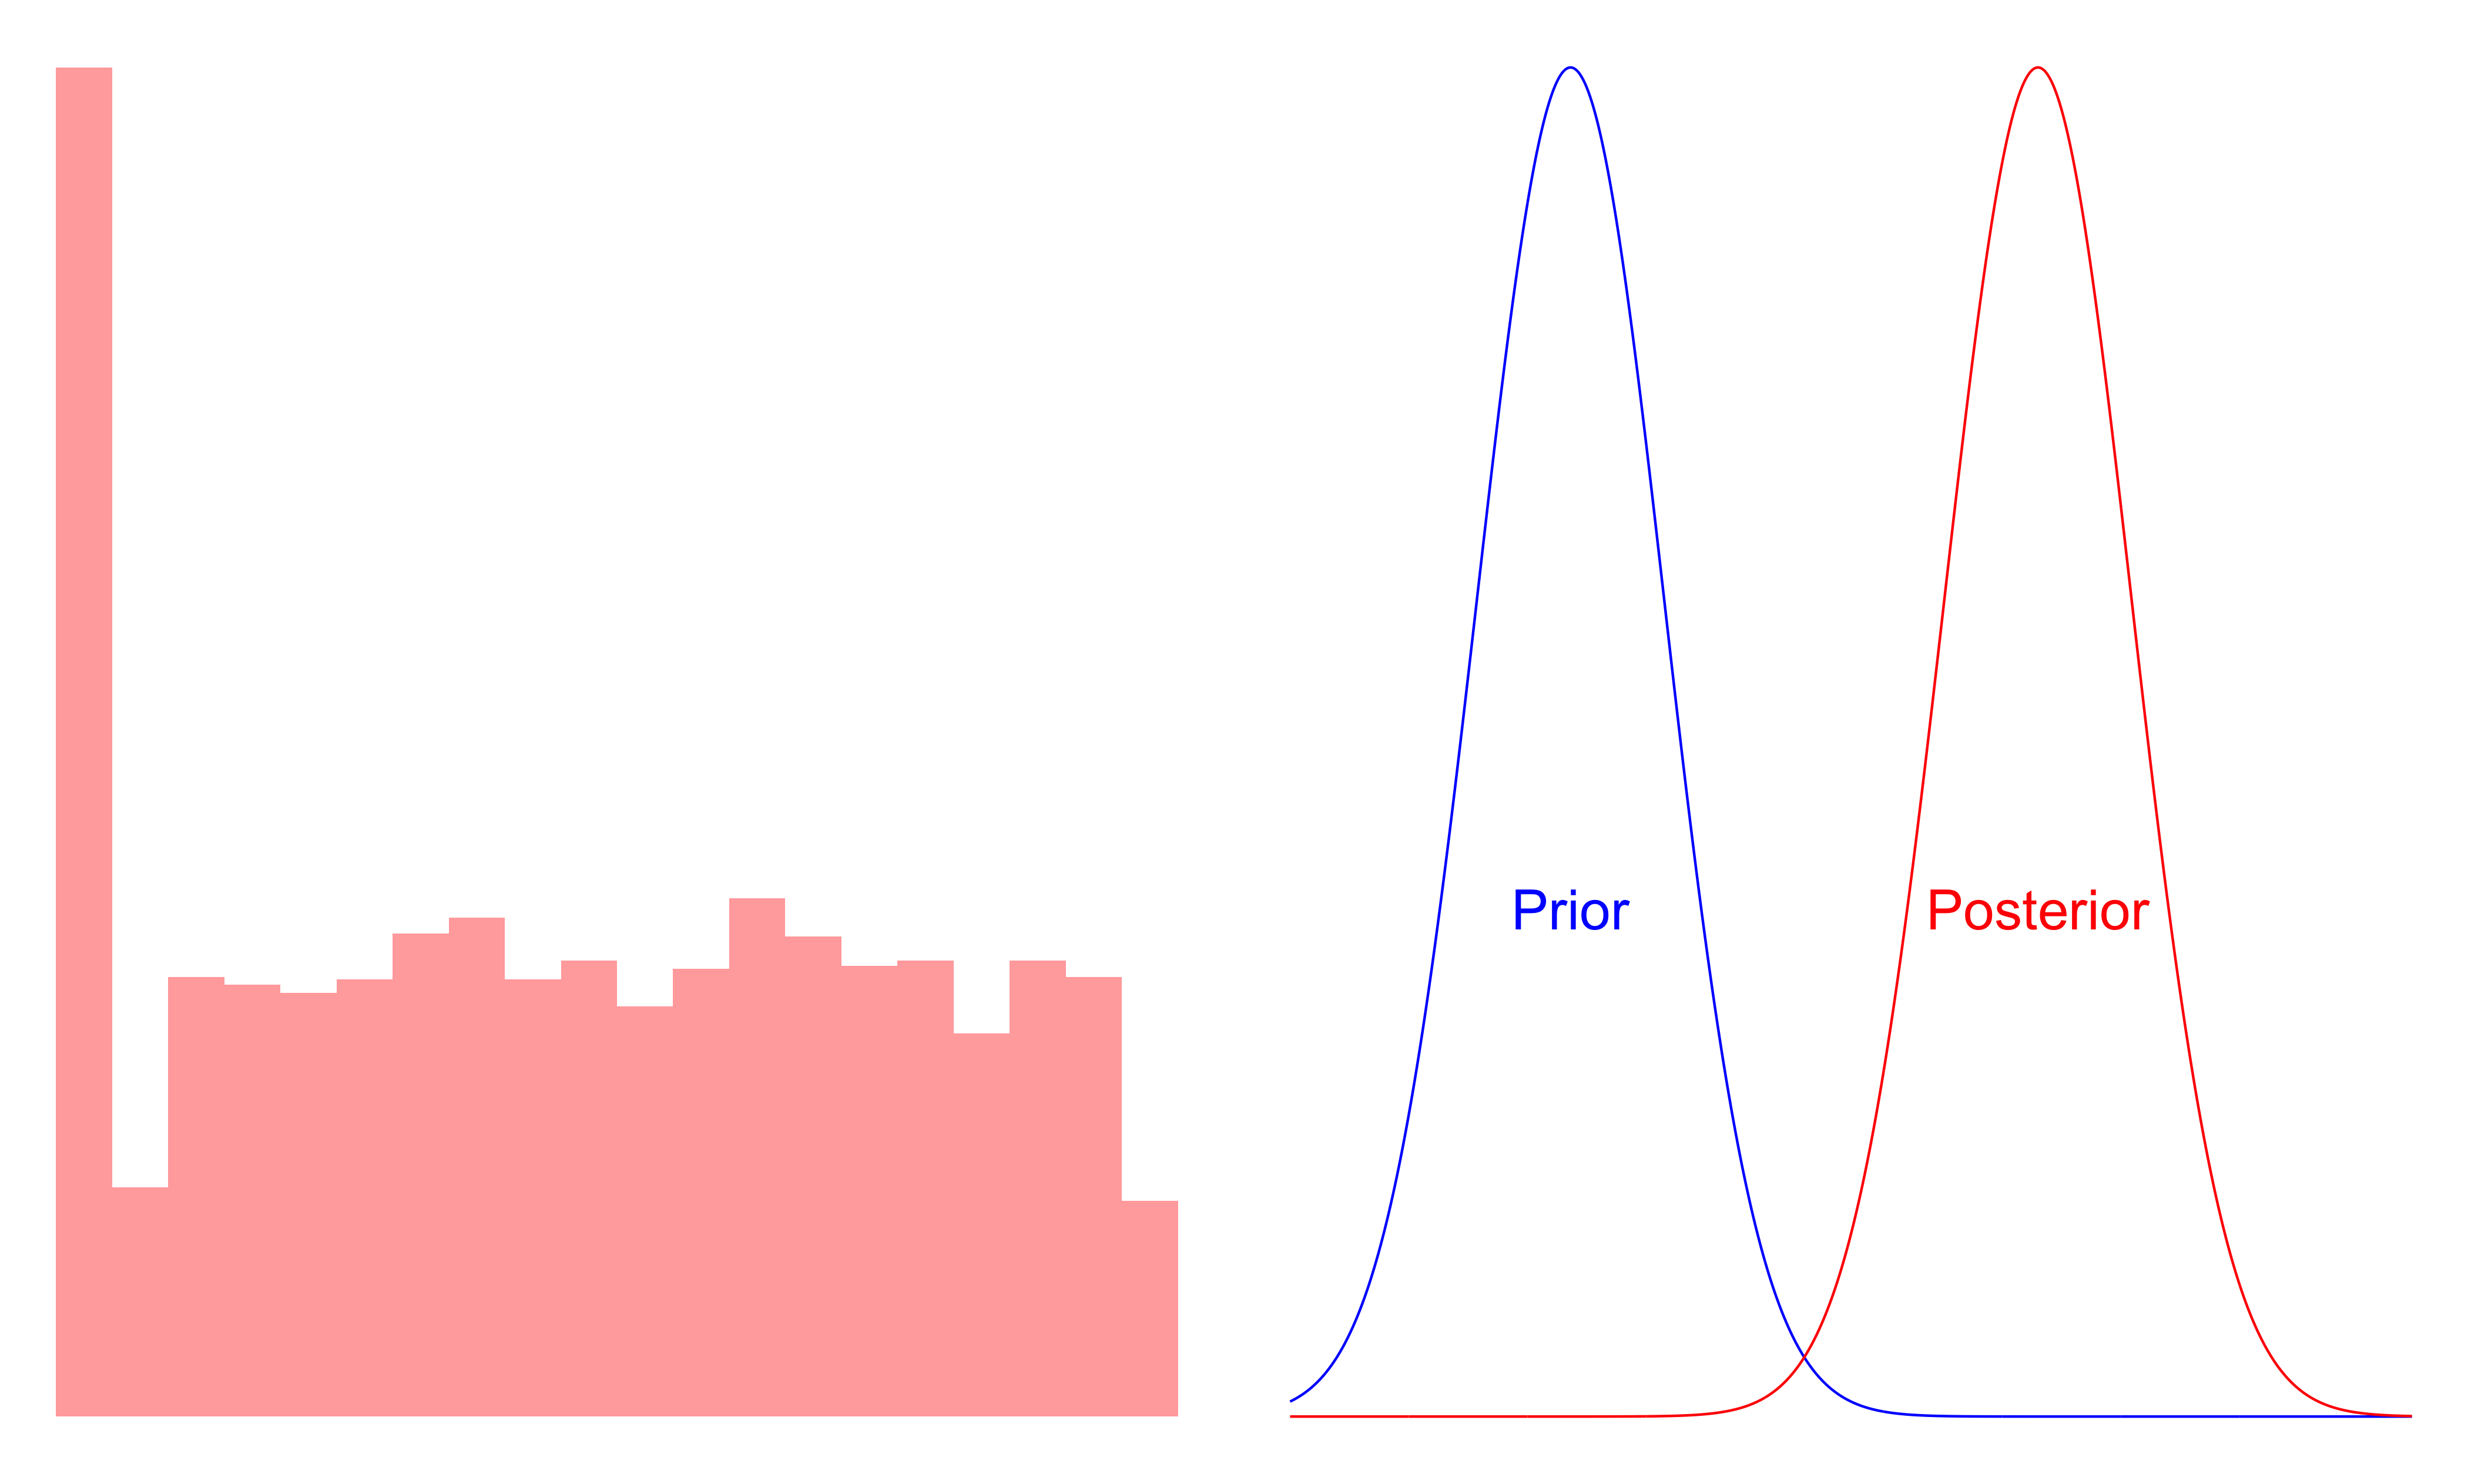
\includegraphics[scale=0.07]{methodology/lhs.png}
            %     \caption{Left: Non uniform rank statistics with peak on the left side. Right: Posterior distribution vertical line representing true parameter. Bias in rank statistics distribution comes from disproportionate number of SBC iterations overestimating the true parameter.}
            %     \label{fig:overestimate}
            % \end{figure}
        
            \begin{figure}[H]
                \centering
                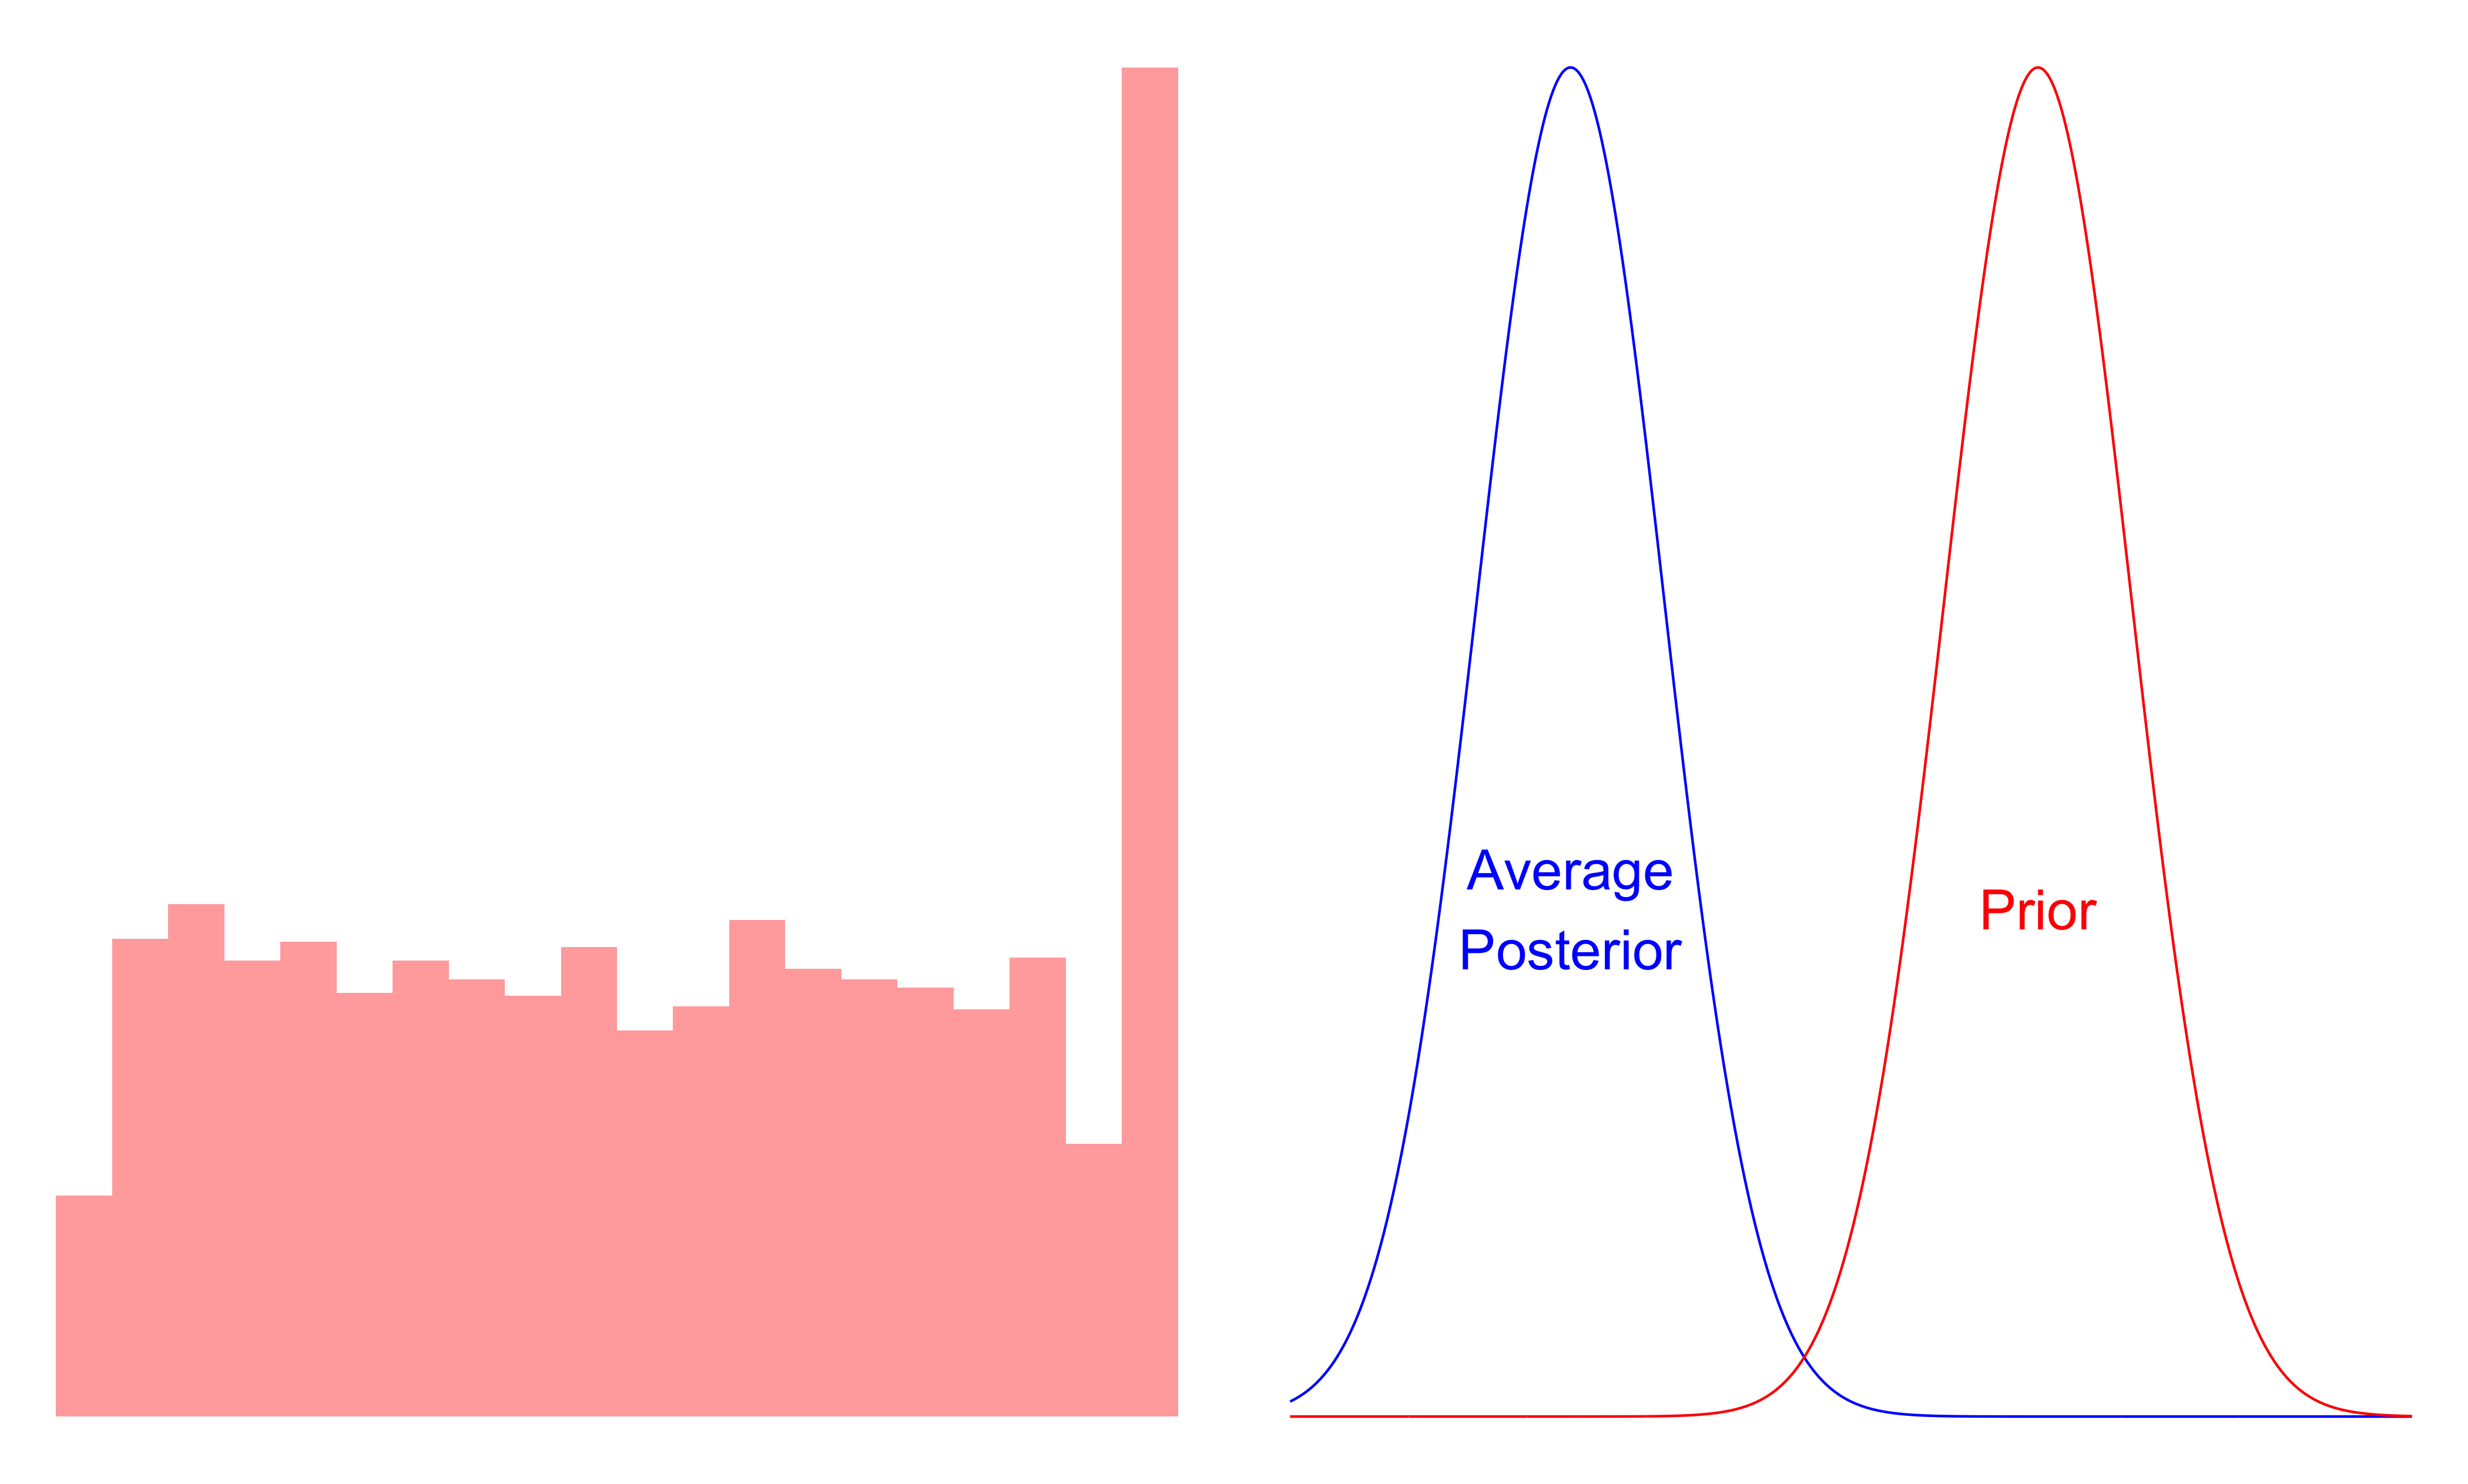
\includegraphics[scale=0.07]{methodology/rhs.png}
                \caption{Left: Non uniform rank statistics with peak on the right side. Right: Posterior distribution is biased to the left side of the prior distribution. Bias in rank statistics distribution comes from posterior samples underestimating the true parameter on average. Note that the two plots are independently produced for illustration only.}
                \label{fig:underestimation}
            \end{figure}        

            \begin{figure}[H]
                \centering
                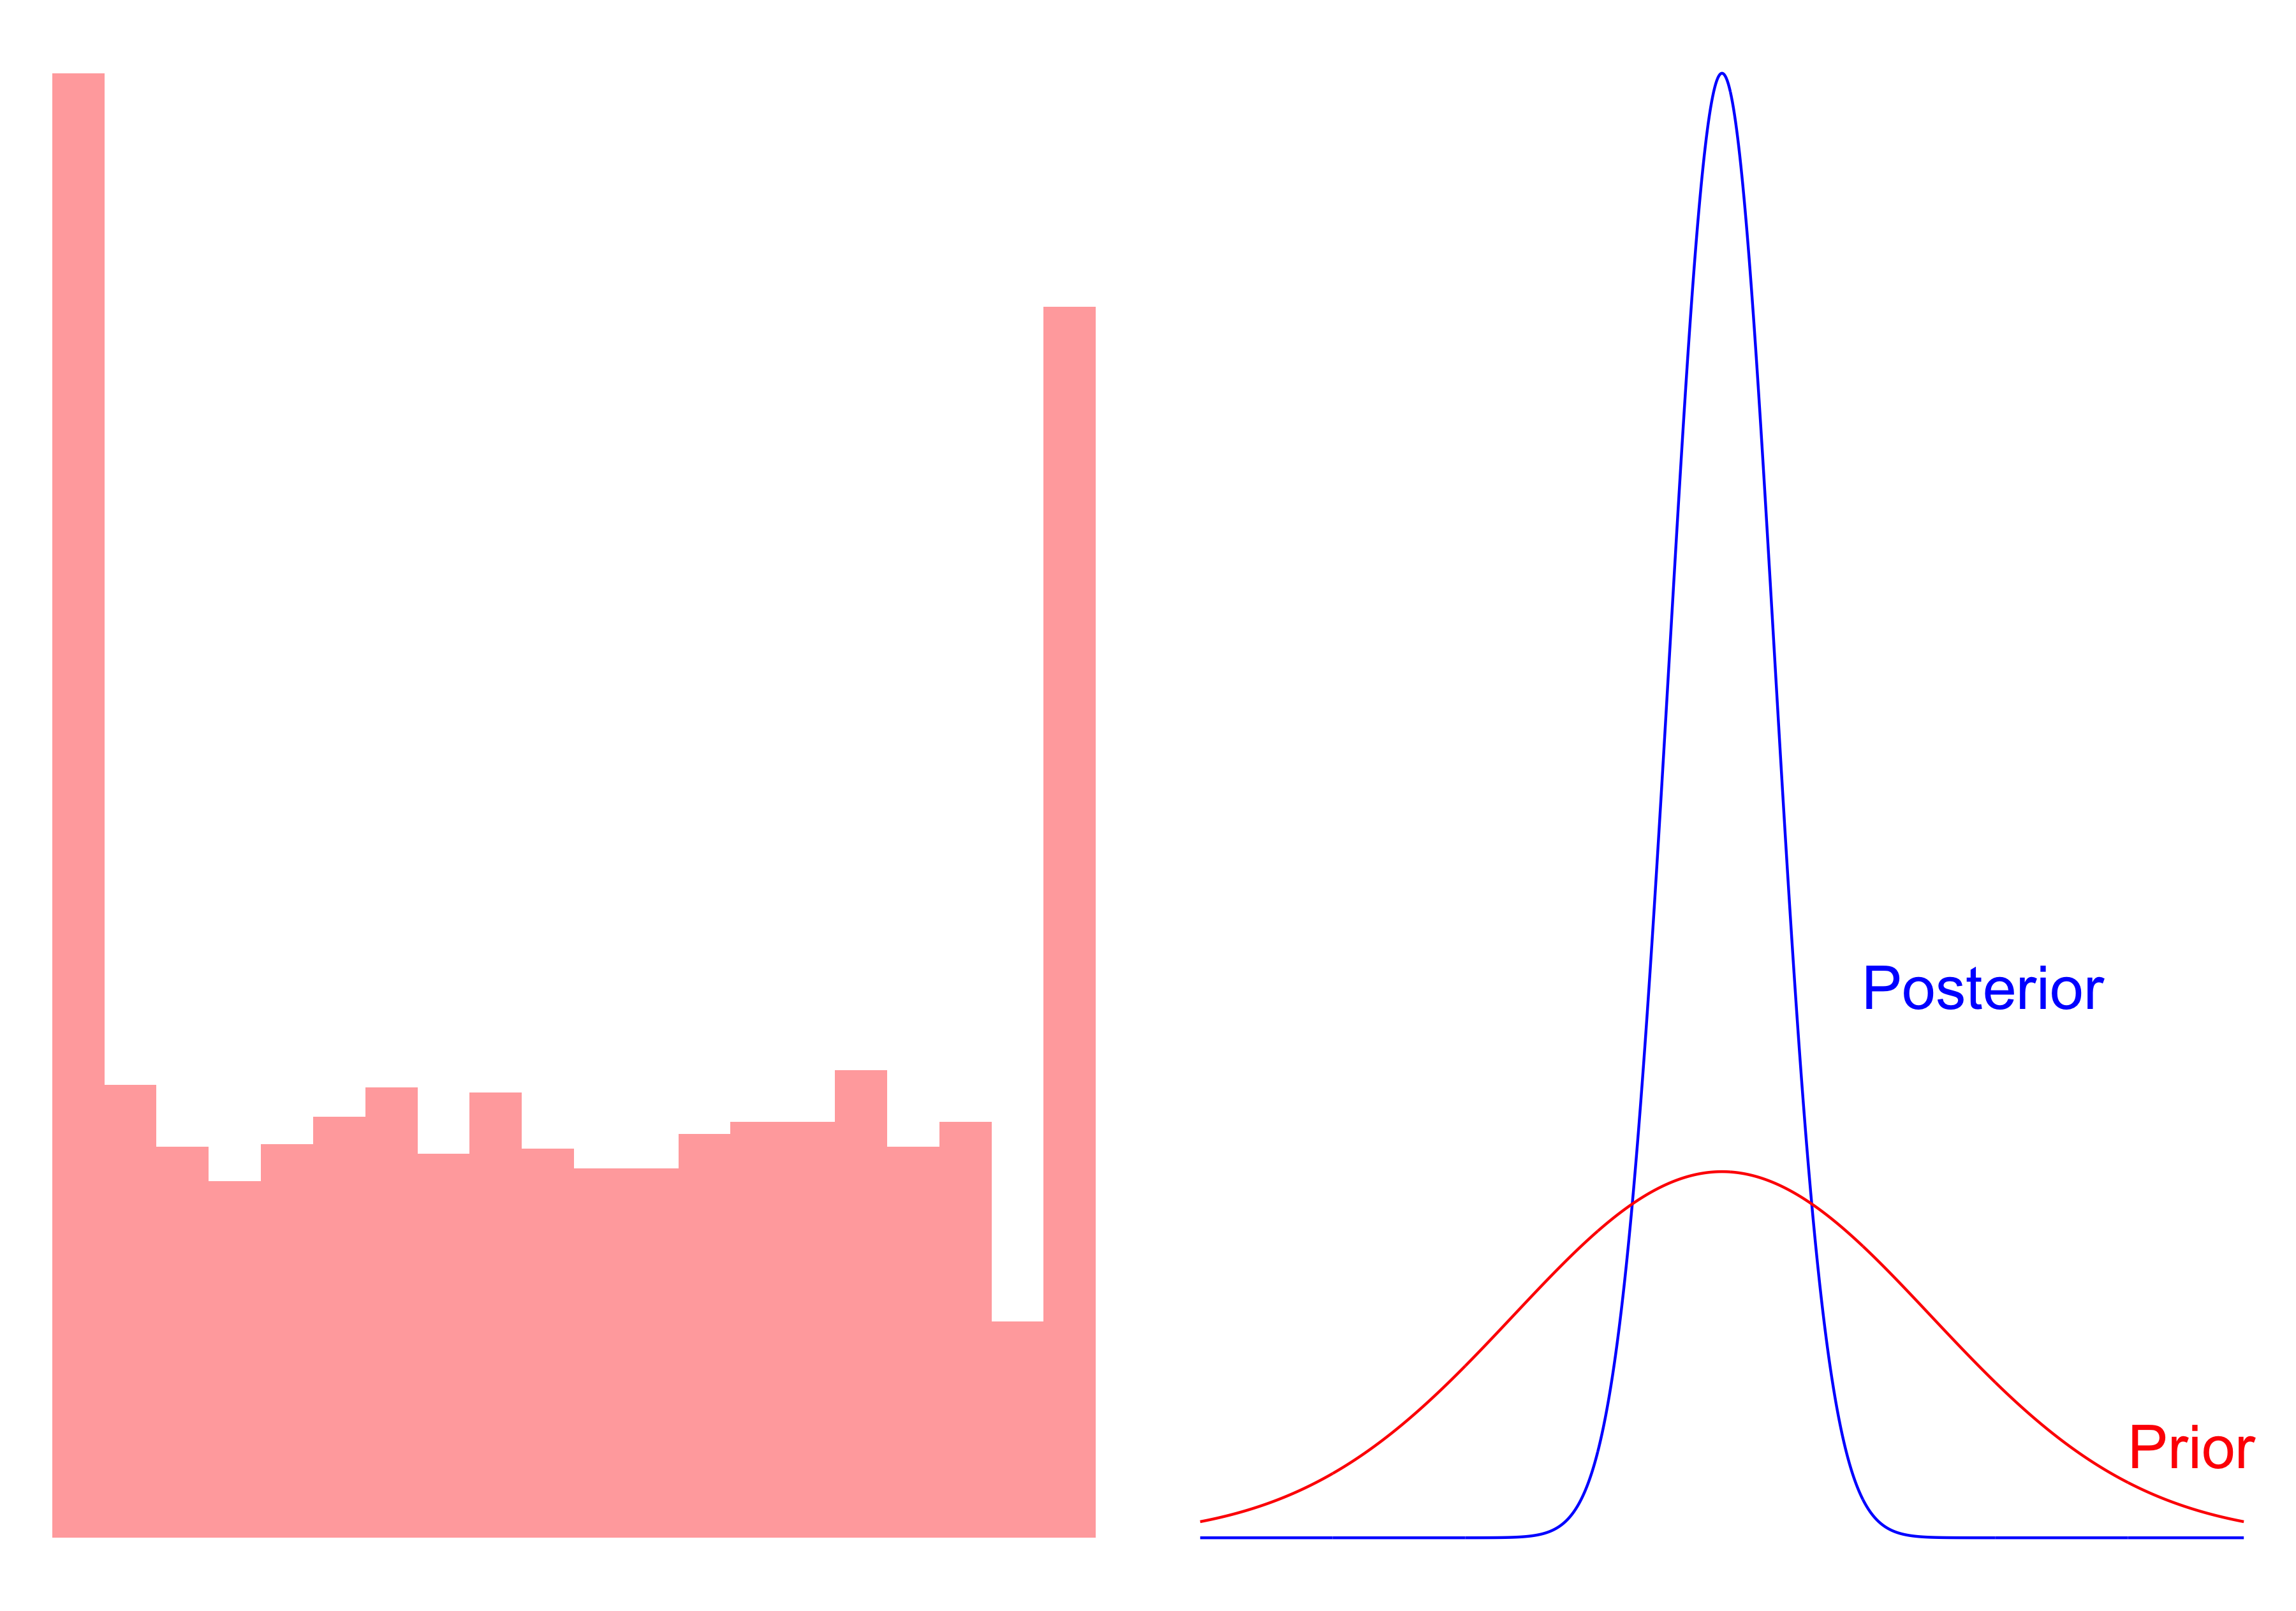
\includegraphics[scale=0.07]{methodology/underdispersed.png}
                \caption{Left: Non uniform rank statistics with peaks on both ends. Right: Overlayed posterior and prior distributions for the same arbitrary parameter. Non-Uniformity in ranks comes from under-dispersed posterior distribution relative to prior.}
                \label{fig:underdispersed}
            \end{figure}

            \subsubsection{Chi squared statistics}
            One difficulty of relying on the visualisation of rank statistic distributions for SV models, is there are a very large number of unknowns in the model to consider. An alternative to visually checking for uniformity of a given parameter is to calculate a chi-squared statistic based on the counts in each histogram bin. Suppose the histogram has $J$ bins, where for each $j^{th}$ bin, $b_j$ is the number of counts and $e_j$ the expected count in bin $j$, where the expected count is the ratio of the number of data points and bins $e_j\frac{T}{J}$. The corresponding chi- squared statistic is given by:
            \begin{align}
            \chi^2 = \sum_{j=1}^J \frac{(b_{j} - e_{j})^2}{e_j}.\end{align}
            
            A discrete empirical distribution with the same number of realisations in each of $J$ bins will return a chi squared statistic of zero, since the number realisations in each bin is equal to the expected count under the relevant  uniform distribution. The distribution of chi squared statistics is visualised to compare results across multiple simulations. Thus, the distribution of chi-squared statistics produced from the histograms of SBC rank statistics for a large number of univariate model parameters will give a high level summary of the overall model calibration, and hence for the overall performance of the algorithm. By comparing the distributions of chi-squared statistic produced by competing algorithms, one algorithm's degree of calibration, relative to that of the other algorithm, may be assessed. 

            \subsubsection{Effective sample size}
            Another univariate summary of a marginal posterior distribution is its effective sample size (ESS), which provides a measure of the efficiency of the MCMC sampler. ESS estimates the number of effectively independent draws generated by a MCMC to estimate a target parameter. A poor ESS generally arises from high auto-correlation in the Markov chain, and thus is an indication of a highly dependent posterior sample. A more efficient MCMC algorithm will take a relatively lower level of resources (for example, time and number of draws) to get a representative sample from the target distribution when compared to a less efficient algorithm. If a MCMC algorithm possesses higher ESS for the majority of its parameters (relative to another strategy), this is seen as evidence of greater efficiency.
            
            The ESS is denoted as $n_{\text{eff}}$. When more than one chain is generated from the target posterior, then the ESS quantity is a function of the number of chains $M$, the number of samples per chain $N$ and the auto-correlation at lag t $\rho_t$ \citep{vehtari2021rank}. $T$ is a truncation lag chosen such that the sum of any two consecutive auto-correlation lags is negative \citep{geyer1992practical}. This truncation (or some kind of down-weighting) is required because a large number of lags leads to noisier auto-correlation estimates. Note that this is only one approach to calculating the ESS. Details about this ESS formula, the calculation of the auto-correlation and other ESS calculations can be found in \citet{vehtari2021rank} and \citet{geyer1992practical}.

            $$
            \begin{aligned}
                n_{\text{eff}} = \frac{NM}{1+2 \sum_{t=1}^T \hat{\rho}_t}
            \end{aligned}
            $$

\section{MCMC Strategies}

    \subsection{Sampling method 1: Mixture off-set MCMC}
        KSC sample the conditional posteriors of the stochastic volatility model using a mix of conjugate posterior distributions, Metropolis Hastings within Gibbs algorithms and an implementation of the Kalman Filter and smoother used to sample from the conditional posterior distribution of the latent states \citep{dejong1995}.\footnote{In this research the exact software to apply the simulation smoother is unavailable. So a more recent simulation smoother is used which is written by the same author of the original software.} Note that for the simulation smoother to produce an appropriate posterior sample draw of the latent state vector, the state and measurement equations are required to be linear and conditionally Gaussian. Since the relationship between $y_t$ and $h_t$ in the measurement equation is not linear, a transformation is applied by squaring and taking the log of $y_t$, resulting in
        \begin{align}
        y_t^{*} &= log(y_t^2) \notag\\ 
        &= log((\epsilon_t exp(h_t/2))^2) \notag\\
        &=  log(exp(h_t)) + log(\epsilon_t^2) \notag\\
        &= h_t + log(\epsilon_t^2) \notag  \\
        &= h_t + z_t,  \label{eqn:transform}
        \end{align}
        Where $z_t = log(\epsilon_t^2)$ has a distribution that is like that of the logarithm of a chi-squared random variable. It is known that the error $z_t$ has mean -1.2704 and variance 4.93, however its distribution is not Gaussian. However, by transforming the entire measurement equation, as in (\ref{eqn:transform}), the relationship between $y_t$ and $h_t$ is now linear; however, the error is not Gaussian. Since it is not simple to sample from this parameterisation of the model, KSC use a mixture of seven Gaussian distributions to approximate the distribution of $z_t$, with the mixture selected to match the first 4 moments of the log chi squared distribution. The mixture distribution is defined by:
        \begin{align}
        f(z_t) = \sum_{i=1}^{K} q_if_N(z_i|m_i-1.2704, \nu_i^2),
        \end{align}
        where $K=7$, $f_N(z|m_i-1.2704, \nu_i^2)$ denotes the density of the normal distribution with mean $m_i-1.2704$ and variance $v_i^2$, and  component probabilities $q_i$, for $k=1,2,\ldots, K=7$.  The values of these hyperparameters and component weights are reported in Appendix A.

        Given a set of $T$ mixture component indicator variables, which are added to the MCMC scheme in order to use the approximating Gaussian mixture error distribution, the latent state vector may be sampled via the Kalman Filter and simulation smoother, since the model is now conditionally linear and Gaussian. The static parameters $\mu$ and $\sigma^2$ are sampled directly from their conjugate posterior distributions whereas $\phi$ is sampled via a Metropolis Hastings accept/reject procedure. Details of the full sampling algorithm are found in Appendix B. 

        \subsubsection*{Implementation}
        The code used to replicate the KSC algorithm was written by \citet{chad2018} and amended for the purposes of this research. Additional code was developed to produce rank statistics, quantities of interest as well as to integrate the sampling method into the SBC framework. 
        
        The steps in the MCMC process is described in Algorithm \ref{alg:ksc}. The initial values are set to the values outlined in \citet{kim1998stochastic}, except for the mixing indicator which is unspecified. This is arbitrarily set at the 4th Gaussian density found in Appendix A.

        For sampling the mixture model the Gaussian mixture density is rewritten with respect to a indicator variable $s_t$
        \begin{align}
        &z_t | s_t = i \sim N(m_i - 1.2704, \nu^2) \\
        &Pr(s_t = i) = q_i.
        \end{align}
        $s_t$ is then sampled from probability mass function: 
        \begin{align}
        Pr(s_t = i | y_t^{\ast}, h_t) \propto q_i f_N(y_t^{\ast} | h_t + m_t - 1.2704, \nu^2).
        \end{align}

        \begin{algorithm}[H]
            \caption{KSC MCMC Algorithm}\label{alg:ksc}
            \begin{algorithmic}
            \Require $s_0 = 4$, $\mu_0 = 0$, $\phi_0 = 0.95$, $\sigma^{2}_{\eta,0} = 0.02$
            \For{\texttt{i in} $1:n_{draws}$}
                    \State \text{Sample states (Kalman Filter and Smoother): } $\boldsymbol{h}_i \sim h|y^{\ast}, s_{i-1}, \phi_{i-1}, \sigma^{2}_{\eta,i-1}, \mu^{i-1}$ 
                    \State \text{Sample mixture indicators: } $s_i \sim s|y^{\ast}, \boldsymbol{h}_{i-1}$
                    \State \text{Sample from conjugate density $\mu$: } $\mu_i \sim \mu|y_{\ast}, s_{i-1}, \phi_{i-1}, \sigma^{2}_{\eta, i-1}, \boldsymbol{h}_{i-1}$
                    \State \text{Sample from conjugate density $\sigma^2_{\eta}$: } $\mu_i \sim \mu|y^{\ast}, s_{i-1}, \phi_{i-1}, \mu_{i-1}, \boldsymbol{h}_{i-1}$
                    \State \text{Sample via Metropolis-Hastings $\phi$: } $\phi_i \sim \phi|y^{\ast}, s_{i-1}, \mu_{i-1}, \sigma^{2}_{\eta, i-1}, \boldsymbol{h}_{i-1}$
                  \EndFor
            \end{algorithmic}
            \end{algorithm}

    \subsection{Sampling method 2: Stan's HMC with No-U-Turn Sampler}
        Hamiltonian Monte Carlo (HMC) is a  general MCMC algorithm used to efficiently sample posterior draws  high associated with high-dimensional and complex stochastic models. Hamiltonian Monte Carlo, originally called Hybrid Monte Carlo, was developed in the physics literature \citep{duane1987hybrid} before being applied in the statistics literature by Radford Neal through his works in Bayesian Neural Networks \citep{neal1995bayesian} and statistical computing \citep{neal2011mcmc}. Versions of this algorithm have since become widely available through open source development projects, including Stan \citep{stan} and PyMC \citep{pymc2023}.

        The key innovation of HMC is that it uses the gradients of the target posterior distribution to generate an efficient path for the sampler to explore. HMC is able to reach more distant points with higher acceptance probabilities than many bespoke MCMC algorithms since its  proposal draws are made using information about the target distribution. Random walk samplers (such as Random Walk Metropolis Hastings) tend to be inefficient in higher dimensions since it becomes more difficult to randomly select a point with a high acceptance probability. The increasing complexity of high dimensions make it harder for a random walk sampler to explore regions over long distances, and thus the sampler tends to become stuck and will require many iterations to converge to the target distribution. 

        A thorough conceptual and theoretical explanation of HMC can be found in \citet{gelman2013bayesian} and \citet{betancourt2017conceptual}. HMC builds upon the Metropolis Hastings algorithm through the introduction of Hamiltonian equations, auxiliary momentum variables $\phi$, and the gradients of the target log posterior distribution. The vector of model parameters $\theta$ is jointly sampled with a vector of momentum variables $\phi$. The momentum variables are also called auxiliary variables since they are required as part of the Hamiltonian equations to generate an efficient proposal but are not a quantity of interest for inference.

        The sampled momentum variable sets out the proposal path for $\theta$ governed by the Hamiltonian dynamics (represented by a set of differential equations). These differential equations are solved using a discrete approximation algorithm, such as a leapfrog integrator, and is a function of the log posterior gradients for a given point $\theta$. The leapfrog integrator has a set of tuning parameters which determines the size and number of steps to be taken along the Hamiltonian path with the final step being the proposal value $(\theta^{\ast}, \phi^{\ast})$. Finally, the Metropolis Hastings accept/reject step is applied using the parameters at the beginning of the leapfrog process $(\theta^{t-1}, \phi^{t-1})$ and the proposal values $(\theta^{\ast}, \phi^{\ast})$. A formal description of the HMC algorithm is provided in Appendix C.

        \subsubsection{Implementation}
        The Stan programming language's implementation of Hamiltonian Monte Carlo will be used for this study. Stan's default algorithm, the No-U-Turn Sampler \citep{hoffman2014no}, allows for direct sampling of the specified stochastic volatility model. The No-U-Turn Sampler (NUTS) proposes the final parameter using multinomial sampling biased towards the second half of the trajectory steps instead of applying the Metrpolis-Hastings step \citep{betancourt2016identifying}. Stan allows for sampling of the generative model and can flexibly handle complicated likelihood functions. 
        
        This approach will also use the same priors as specified in the KSC's Gaussian mixture approximation so that HMC is sampling from the same model (although other priors could be chosen). 

    \subsection{MCMC methods comparison}
        The KSC sampling method and HMC are both MCMC strategies to generate samples from the target joint posterior distribution of the stochastic volatility model. However, the two sampling approaches are conceptually different in their design and implementation, despite sharing the same objective.
        
        The KSC sampling method is a bespoke algorithm designed specifically for the sampling of the stochastic volatility model. It is a strategy built around how to sample the parameters from the state space model in this specific context. The implementation of this MCMC requires careful attention to the sampling of each parameter using different tools and requires these components to be programmed manually, such as the Metropolis Hastings step and conjugate posterior distributions. 
    
        HMC on the other hand is a more general approach to applying MCMC. The implementation of HMC is through the Stan programming language which allows for the specification other generative or Bayesian models, not just stochastic volatility. The implementation details of HMC is abstracted away from the user, who only needs to focus on specifying the model using the Stan syntax. Any hyper-parameter tuning and initialisation is automated. Furthermore, Stan and HMC allows for the specification of different priors, whereas KSC's bespoke algorithm is dependent on the use of conjugate priors. 

        The conceptual difference in both methods result in different trade-offs. The abstraction of the MCMC implementation using the Stan programming language means users can focus more on the modelling and the applied research question. The algorithm is maintained and thoroughly tested by developers and different models can be compared with each other without worrying about differences in MCMC implementations. However, the abstraction away from the details means there is less flexibility in MCMC design in the scenario where the current instance of Stan or HMC is insufficient for a specific model.
        
    \subsection{Model Parameterisation}

        The parameterisation of a model can affect the performance of a MCMC algorithm when sampling from models with complex posterior geometries. An example of this is Neal's funnel \citep{neal2003slice} where the Hamiltonian Monte Carlo sampler encounters performance issues in hierarchical models and produces biased samples. Efficiency improvements of MCMC algorithms for state space models under different parameterisations are also explored in \citet{strickland2008parameterisation}.

        The stochastic volatility model as described in section 2.1 follows a centered parameterisation. This describes the central location of the latent state distribution which is centered on the mean of log volatility $\mu$. A model can be re-parameterised in a way that might improve MCMC performance. Reparamaterisation applies a transformation to the model which may change the interpretation of the parameters or the way they are sampled but remains mathematically equivalent to the original model. The reparamaterisation available for a model is dependent on the MCMC approach. Some reparamaterisation are available only to specific sampling strategies and may improve or impair a MCMC performance. 

        SBC is applied to reparamaterised versions of the stochastic volatility model to see if there is any improvement in calibration and efficiency. 
        
        \subsubsection{Reparamaterised stochastic volatility in Stan}
        The reparamaterisation for Hamiltonian Monte Carlo changes how the latent states are sampled. Specifically, the states are first sampled from a standard normal distribution and are transformed to be samples from the state equation. As noted above, the centered paramaterisation samples the states centered around $\mu$.  

        First sample from a standard normal distribution and multiply by the variance of the log volatility. The state vector is sampled with mean centered on zero and variance equal to $\sigma_{\eta}^2$

        $$
        \begin{aligned}
        h_{std} \sim & \space normal(0,1) \\
        h =& h_{std} \times \sigma_{\eta}
        \end{aligned}
        $$
        
        Then apply the appropriate re-scaling to get samples from log volatility. 
        
        $$
        \begin{aligned}
        h_1 =& \space \frac{h_{std, 1}\times \sigma_{\eta}} {\sqrt{1 - \phi^2}} + \mu \\
        h_{t+1} =& \space h_{std, t+1}\times \sigma_{\eta} + \mu  + \phi(h_{t} - \mu),\space t\neq 1
        \end{aligned}
        $$
        
        This returns log volatility as desired.
        
        \subsubsection{Non centered Gaussian Mixture model}
        The re-parameterised model for the Gaussian approximation is expressed differently due to the Kalman Filter. Re-parameterised HMC samples from the joint posterior directly with state vectors centered at zero and transformed to return the correct log volatility estimates. Applying the Kalman Filter requires the state equation to be a function of the state variable with the average log volatility parameter $\mu$ entering the measurement equation.

        The following parameterisation is described as non centered in location. This follows the methodology outlined in \citet{strickland2008parameterisation}.
        
        Starting with the log chi squared model:

        $$
        \begin{aligned}
        y^{\ast}_t =& h_t + z_t \\
        h_{t+1} =& \space \mu +\phi(h_t - \mu) + \sigma_{\eta} \eta_t
        \end{aligned}
        $$
        

        Let $g$ be the demeaned state variable. Rewrite the demeaned state equation $g_{t+1}$ to be non centered in location by subtracting average volatility $\mu$.

        $$
        \begin{aligned}
        g_t =& h_t - \mu \\
        g_{t+1} =& \phi g_t + \sigma_{\eta}\eta_{t}
        \end{aligned}
        $$

        Return average volatility into measurement equation and rewrite as a function of the non centered state equation:

        $$
        \begin{aligned}
        y^{\ast}_t =& g_t + \mu + z_t \\
        g_{t+1} =& \phi g_t + \sigma_{\eta}\eta_{t}
        \end{aligned}
        $$

        The mean of the log volatility is now inside the measurement equation and de-meaned from the state equation.
    
    \subsubsection{Prior Predictive check}
        % Different parameteristions express the same mathematical models in ways that make it easier or harder for a given algorithm to sample. 
        A prior predictive simulation of the second state parameter is performed for both a centered and re-parameterised model using the approach described in Section 4.4.1. This is to demonstrate that different parameterisations express the same underlying mathematical model. This is similar the first two steps of SBC, except instead of generating a data set, generate the state variable implied by the prior draw. Let $\boldsymbol{\theta}$ be a vector of static parameters. Simulate a draw from the joint prior:

        $$
        \begin{aligned}
        \boldsymbol{\theta}^{sim} \sim \pi(\boldsymbol{\theta})
        \end{aligned}
        $$

        Generate a the second state parameter conditional on prior simulation and first state variable.

        $$
        \begin{aligned}
        h_2^{sim} \sim \pi (h_2|h_1, \boldsymbol{\theta}^{sim})
        \end{aligned}
        $$

        Simulating 5000 samples of $h_2^{sim}$ from both centered and non-centered models gives samples from the same data generating process as shown in Figure \ref{fig:priorpred}. 


        \begin{figure}[h]
            \centering
            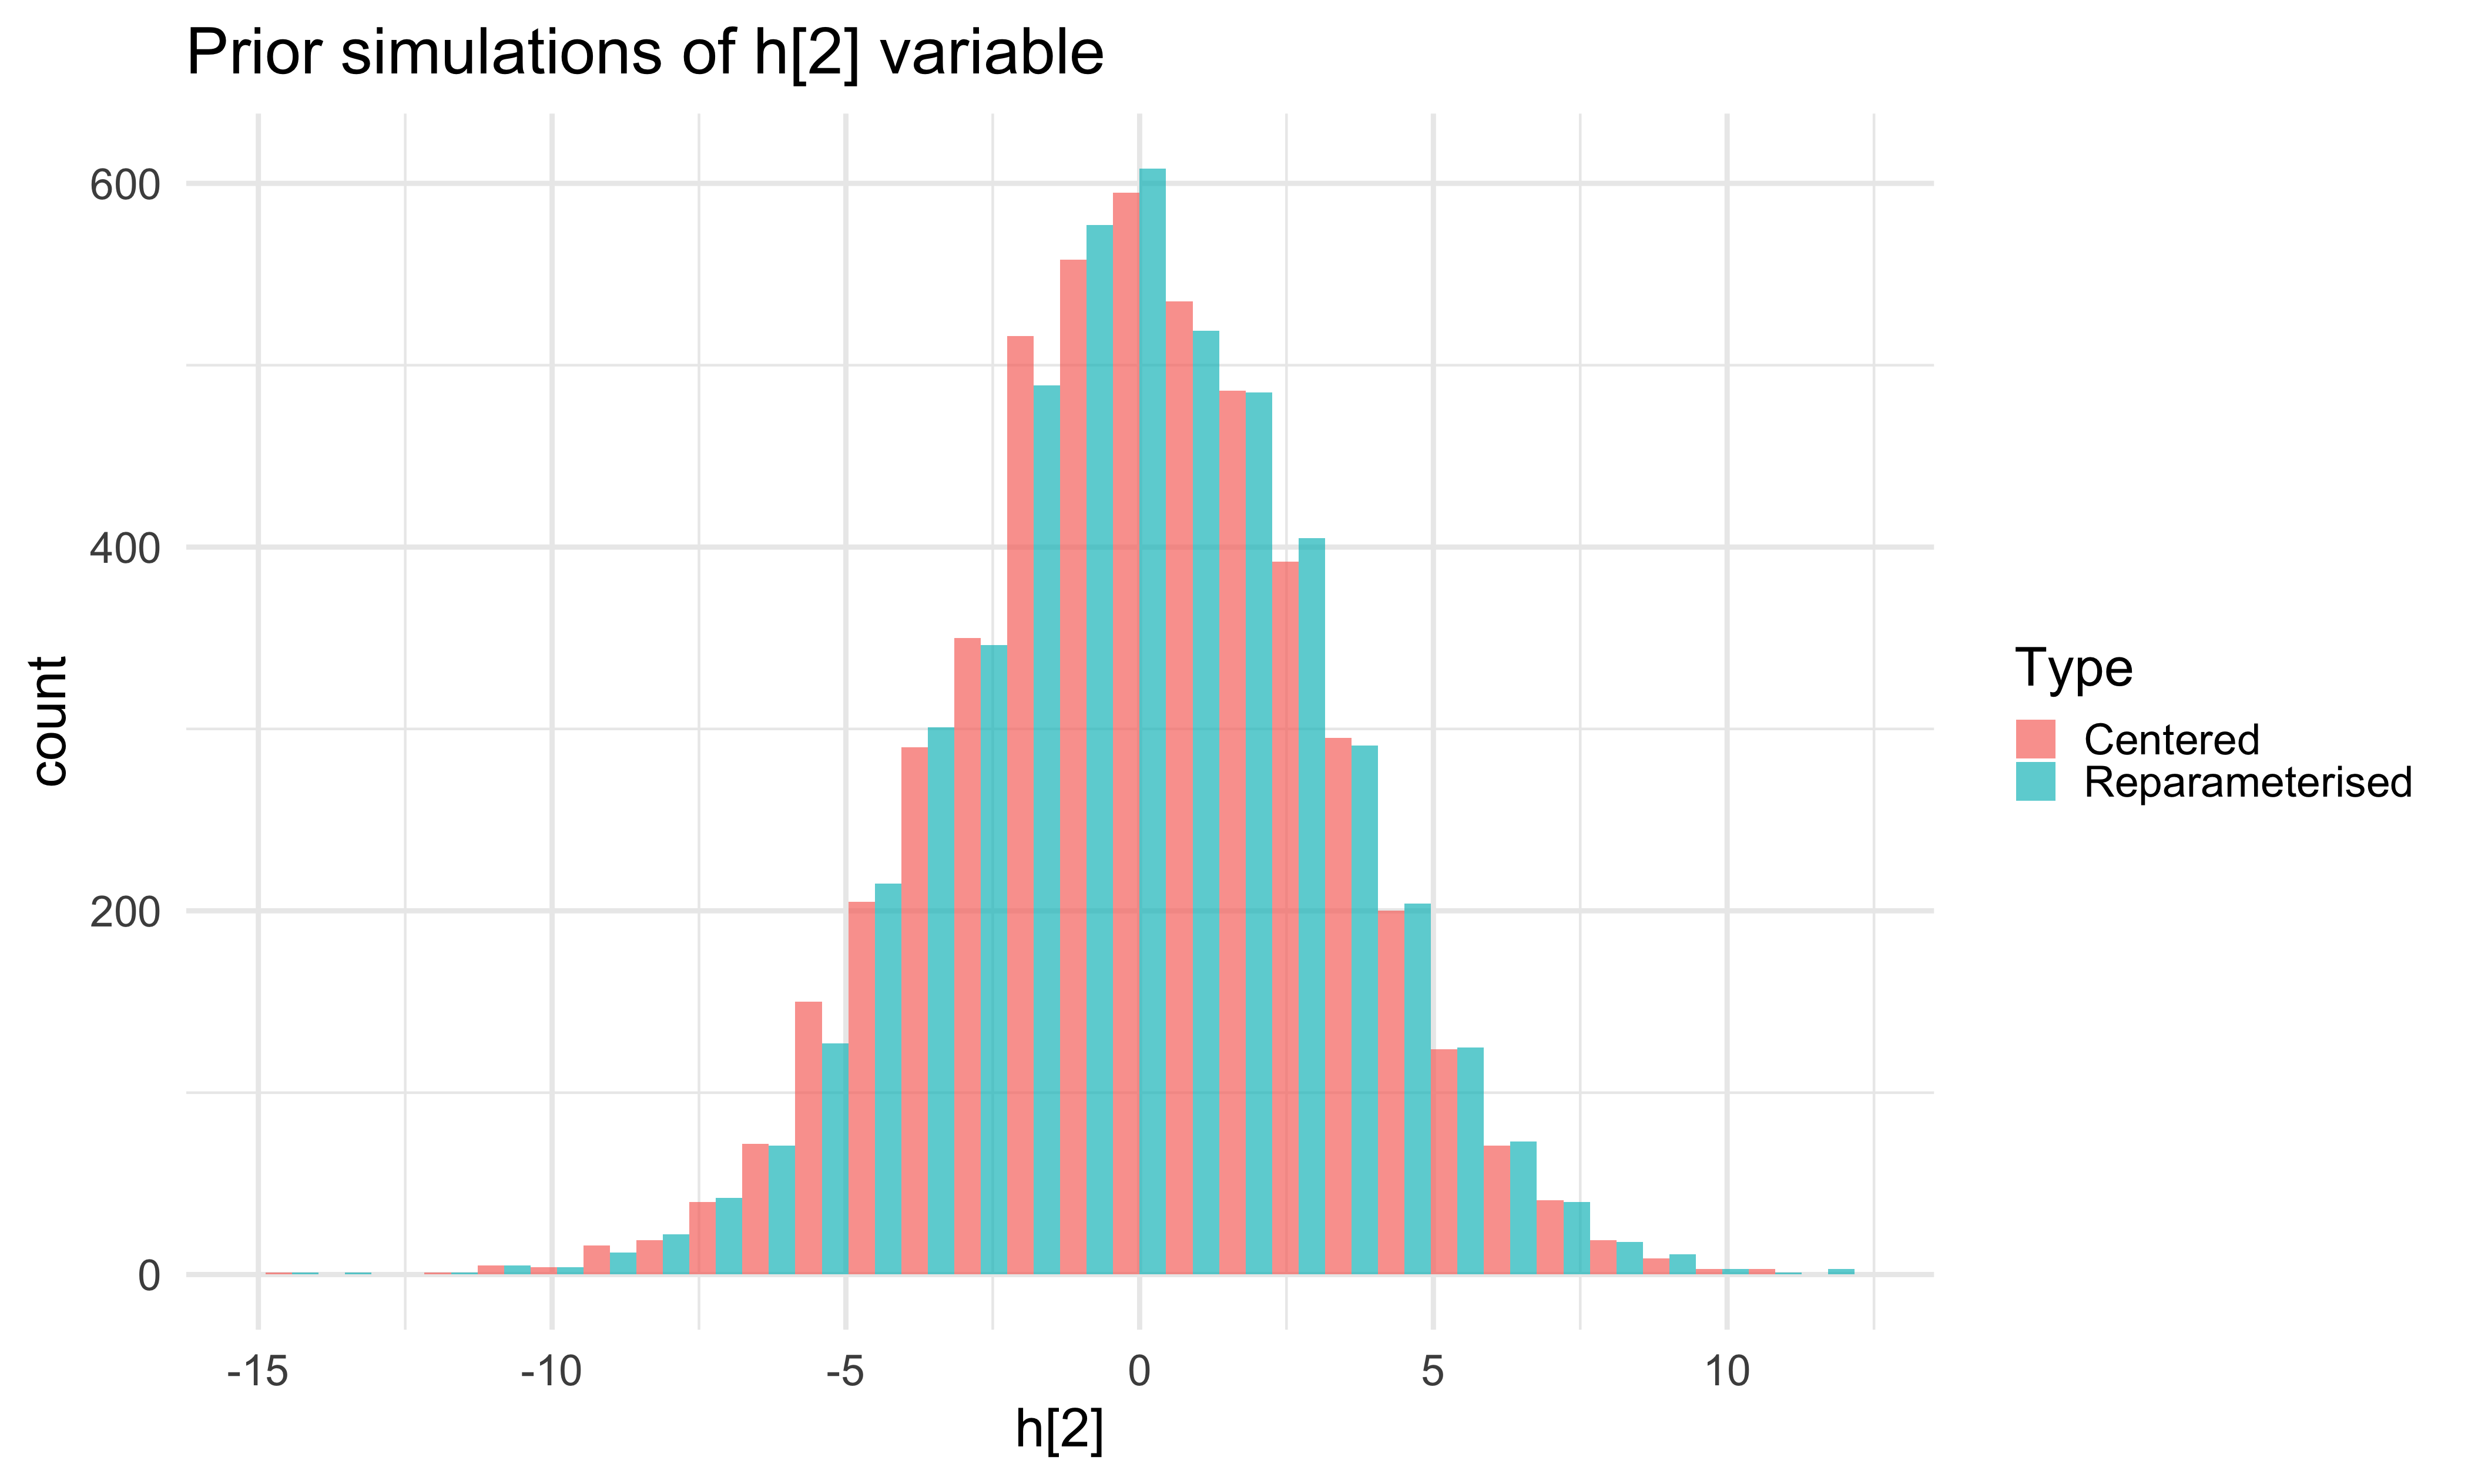
\includegraphics[scale=0.1]{figures/ppc_h2.png}
            \caption{Prior predictive simulation of second state variable from both centered and re-parameterised stochastic volatility model. Both models are mathematically equivalent and generate samples from the same data generating process.}
            \label{fig:priorpred}
        \end{figure}
        
        % Emphasise here that different paramterisations of the models are the same model
        % Use a prior predictive check from both paramterisations show that the results are
        % the same



\section{Results}
    1000 and 5000 SBC iterations are run for centered and re parameterised versions of the stochastic volatility model using simulated data sets of 1000 observations. Rank statistic histograms are constructed with 20 bins for the static parameters and the 1st, 500th and 1000th latent state variables. The black horizontal line represents uniformity conditional on the number of bins and SBC iterations. The $\chi^2$ statistic is used to summarise the deviations from uniformity for all state variables since it is unrealistic to visually inspect all the histograms. The SBC algorithm is summarised Algorithm \ref{alg:sbc}:

    \begin{algorithm}
        \caption{SBC}\label{alg:sbc}
        \begin{algorithmic}
        \For{\texttt{i in} $1:1000$}
                \State \text{Draw from joint prior: } $\boldsymbol{\theta}^{sim}_i \sim\pi (\boldsymbol{\theta})$
                \State \text{Simulate dataset with 1000 observations: } $\boldsymbol{y}^{sim}_i \sim p(y|\boldsymbol{\theta}^{sim}_i)$
                \State \text{Draw 999 posterior samples post burn in:} $\{\boldsymbol{\theta}_1,\dots , \boldsymbol{\theta}_{999}\}_i \sim p(\theta | \boldsymbol{y}^{sim}_i)$
                \State \text{Compute rank statistics:} $\boldsymbol{r} = rank(\{\boldsymbol{\theta}_1,\dots , \boldsymbol{\theta}_{999}\}_i, \boldsymbol{\theta}^{sim}_i)$
              \EndFor
        \end{algorithmic}
        \end{algorithm}
        
    \subsection{Hamiltonian Monte Carlo}
    Figure \ref{fig:cphmc1k} and Figure \ref{fig:ncphmc1k} show the SBC results for the centered and re-parameterised model for HMC respectively. Both sets of results display relatively noisy rank statistic estimates with variation around the discrete uniform distribution.

    The centered parameterisation in particular displays a lack of uniformity for $\phi$ and $\sigma^2$. Rank statistics for $\sigma^2$ and $\phi$ show two peaks of either end of the histogram. The posterior estimates of $\sigma^2$ and $\phi$ are \textit{under-dispersed} relative to the prior distribution. This implies the posterior geometry of these parameters may be difficult to sample for the HMC algorithm.

    \begin{figure}[H]
        \centering
        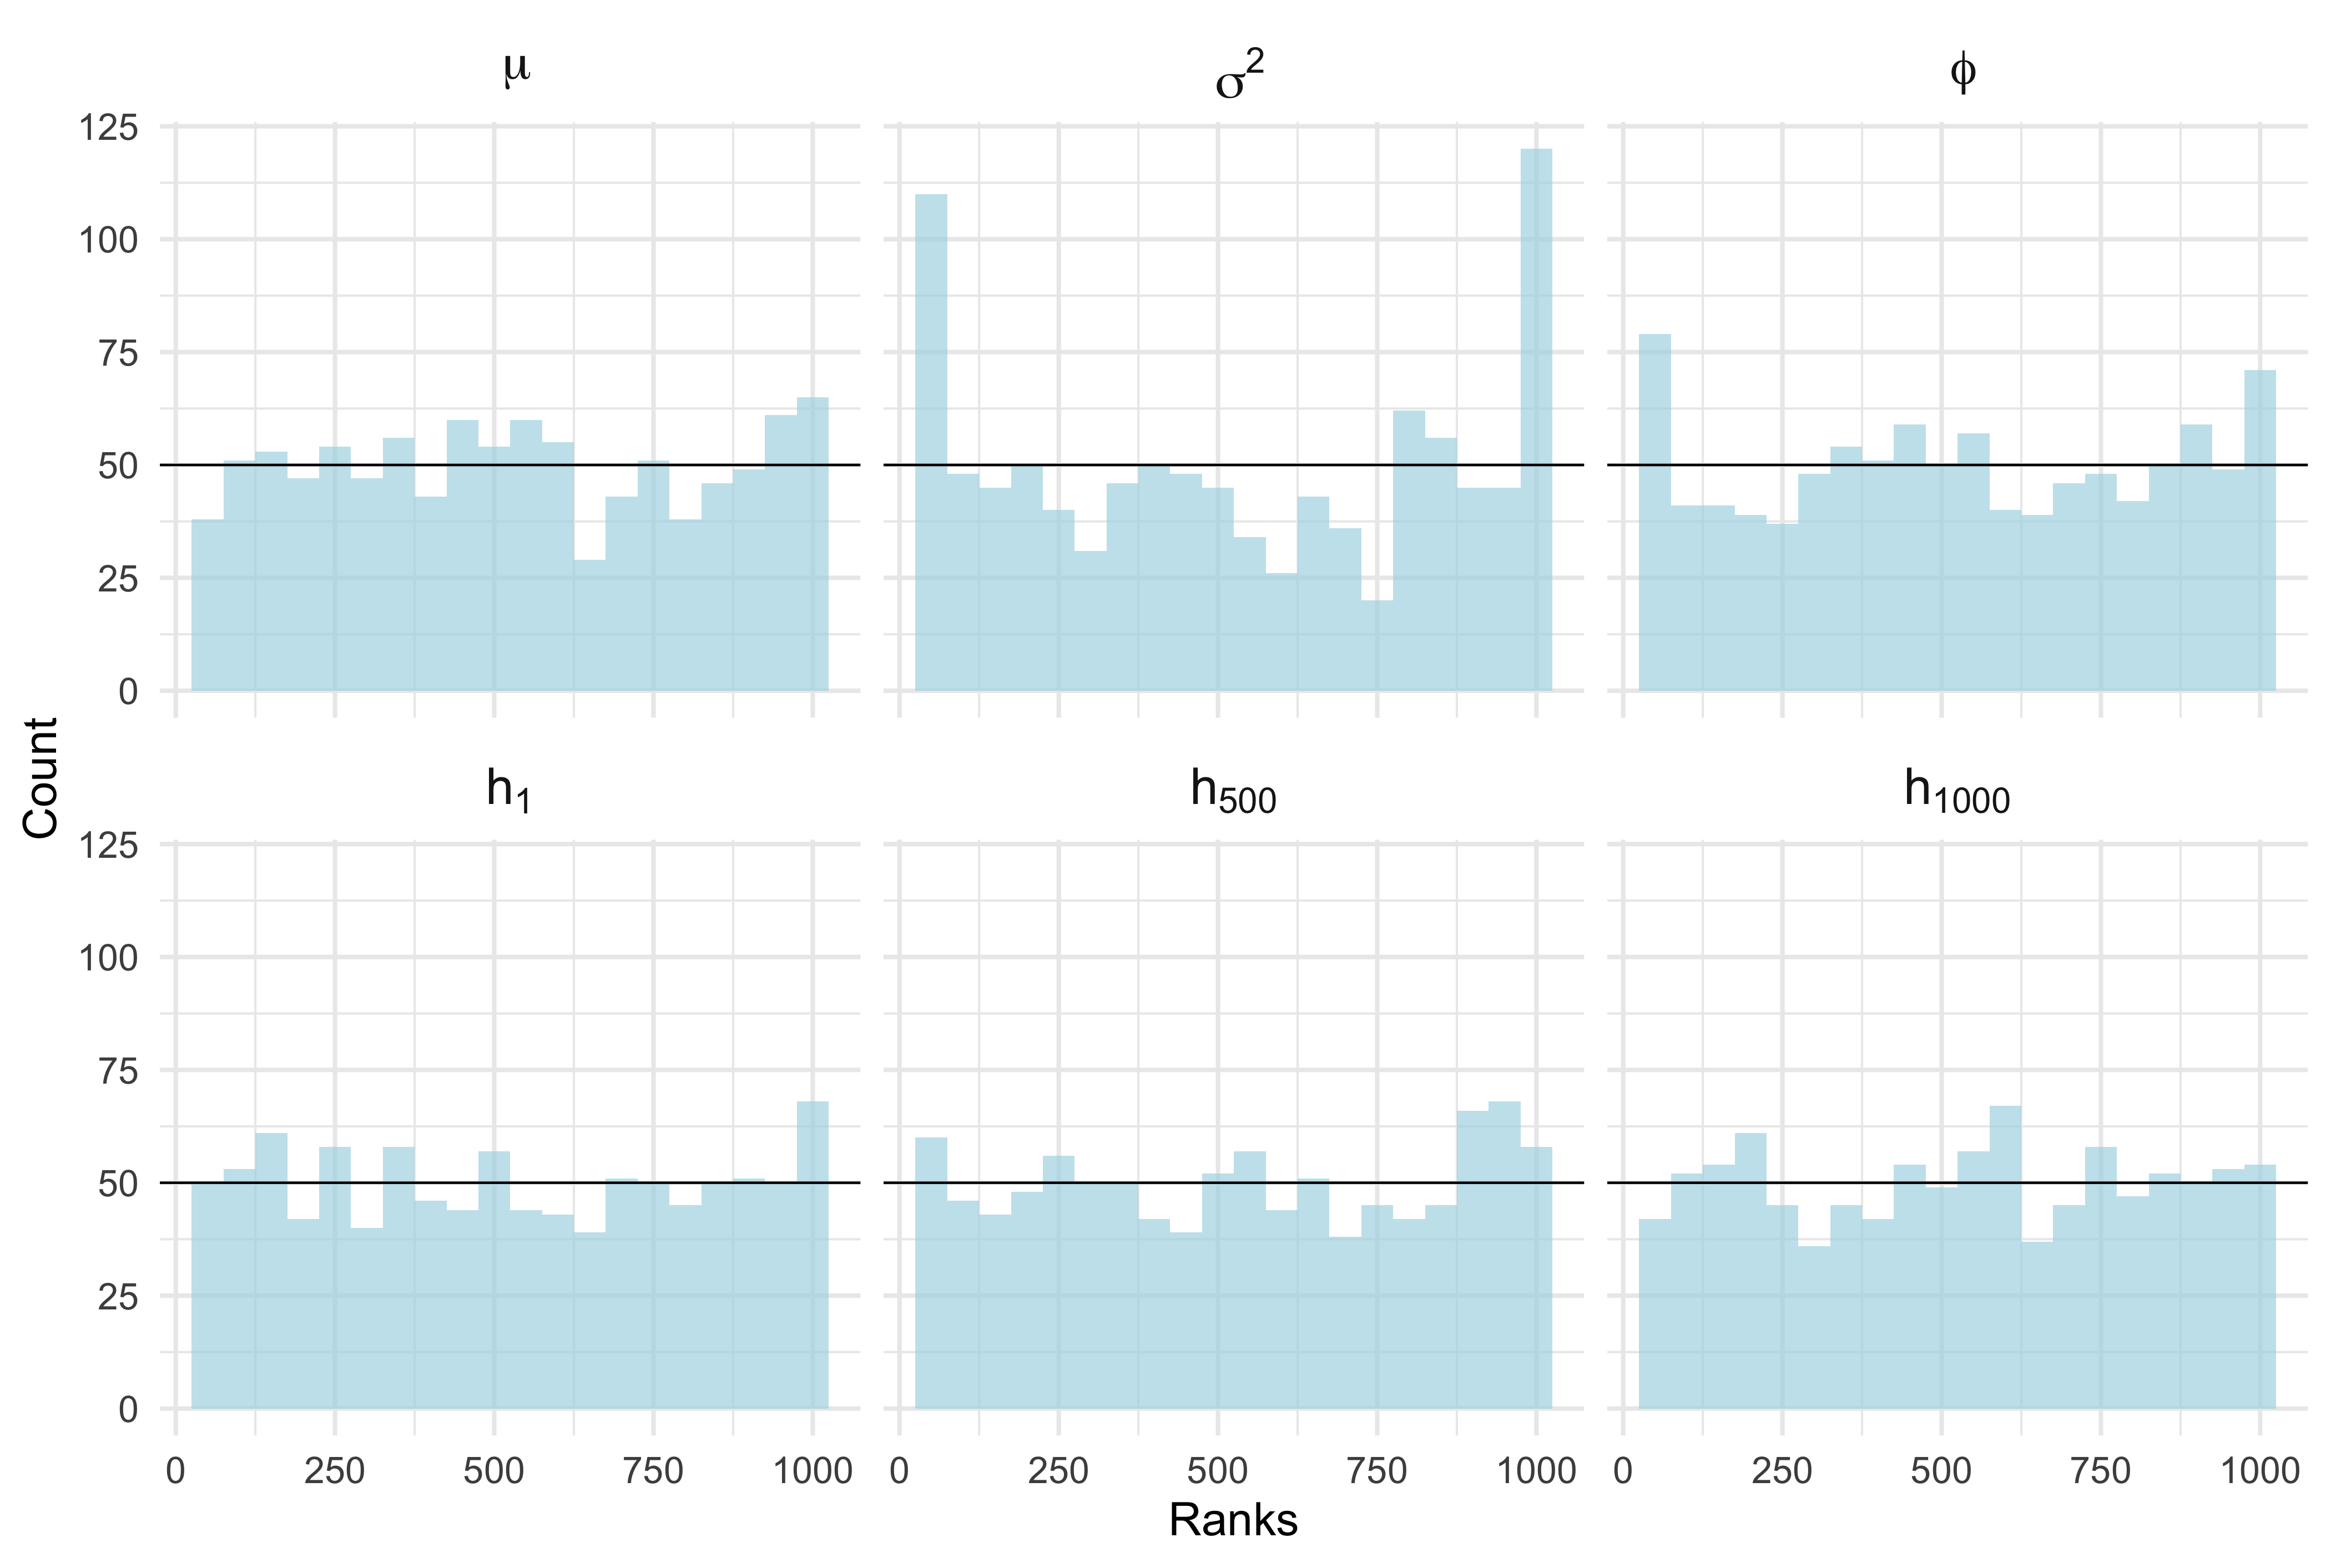
\includegraphics[scale=0.09]{results/hmc_cp_1k.png}
        \caption{1000 SBC iterations for centered model using Hamiltonian Monte Carlo. Histograms show noisy estimates around uniform distribution. In particular, $\sigma^2$ displays peaks on both ends of the histogram and $\phi$ shows a major on the left hand side. This suggests that the posterior samples of $\sigma^2$ are under-dispersed relative to the prior distribution and posterior samples of $\phi$ are over estimating the true parameter.}
        \label{fig:cphmc1k}
    \end{figure} 

    Estimates of $\sigma^2$ and $\phi$ are more uniform under the re-parameterised model. Instead, we observe a peak on the left side for the 500th state variable $h_{500}$, although the estimates are noisy. Overall the estimates for non centered parameterisation are more favourable. 

    \begin{figure}[H]
        \centering
        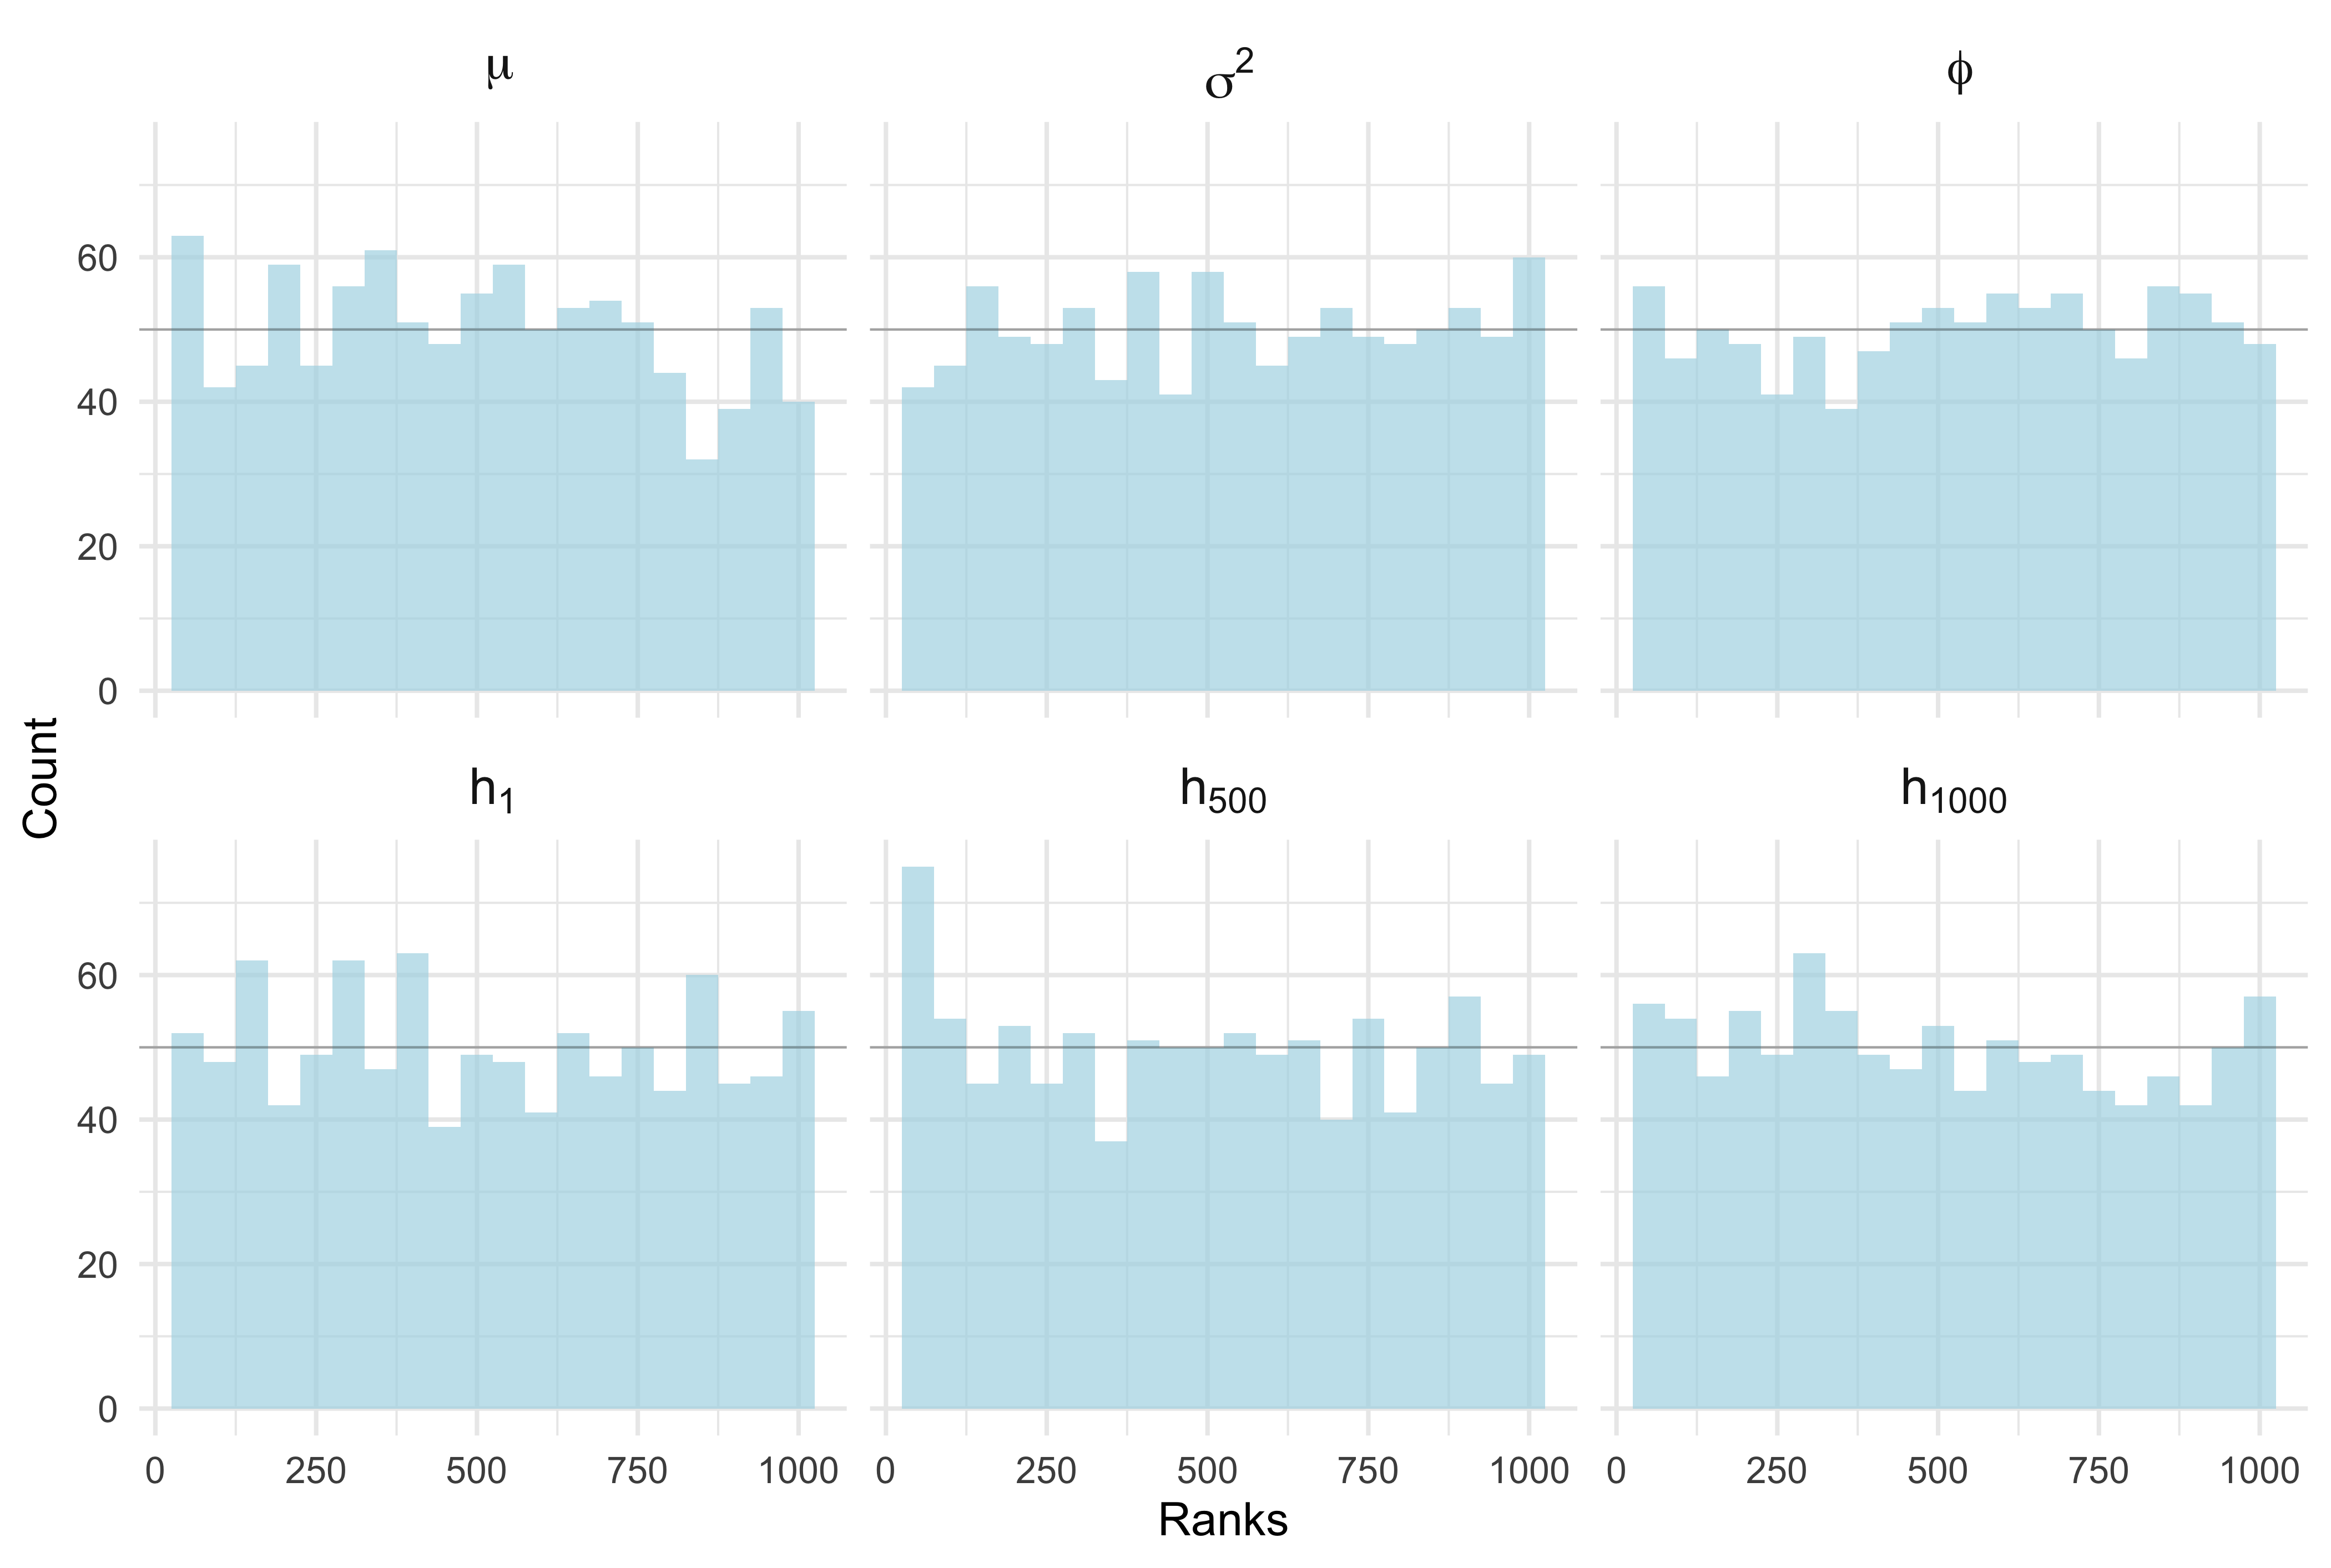
\includegraphics[scale=0.09]{results/hmc_ncp_1k.png}
        \caption{1000 SBC iterations for non centered model using Hamiltonian Monte Carlo. The rank statistic distributions for $\sigma^2$ and $\phi$ have improved. There is some evidence that the posterior of the 500th state variable is overestimating the distribution of its true value.}
        \label{fig:ncphmc1k}
    \end{figure}

    The noisy histogram estimates can be improved by increasing the number of SBC iterations. Figure \ref{fig:cphmc5k} and Figure \ref{fig:ncphmc5k} show the results of the same parameters with 5000 SBC iterations. There is an improvement to the re-parameterised model with all histograms looking approximately uniform with much smaller variation around the uniform distribution. 
    
    Centered parameterisation posses similar improvement for $\mu$ and the state variables. However, there are still major peaks at both ends of $\sigma^2$ and $\phi$ suggesting under-dispersion of the posterior estimates relative to the prior distribution.

    These results suggests that HMC struggles to sample some parameters from the centered parameterisation of the stochastic volatility model. The re-parameterised model possess stronger evidence of calibration for the parameters examined, implying more reliable and consistent inference.

    \begin{figure}[H]
        \centering
        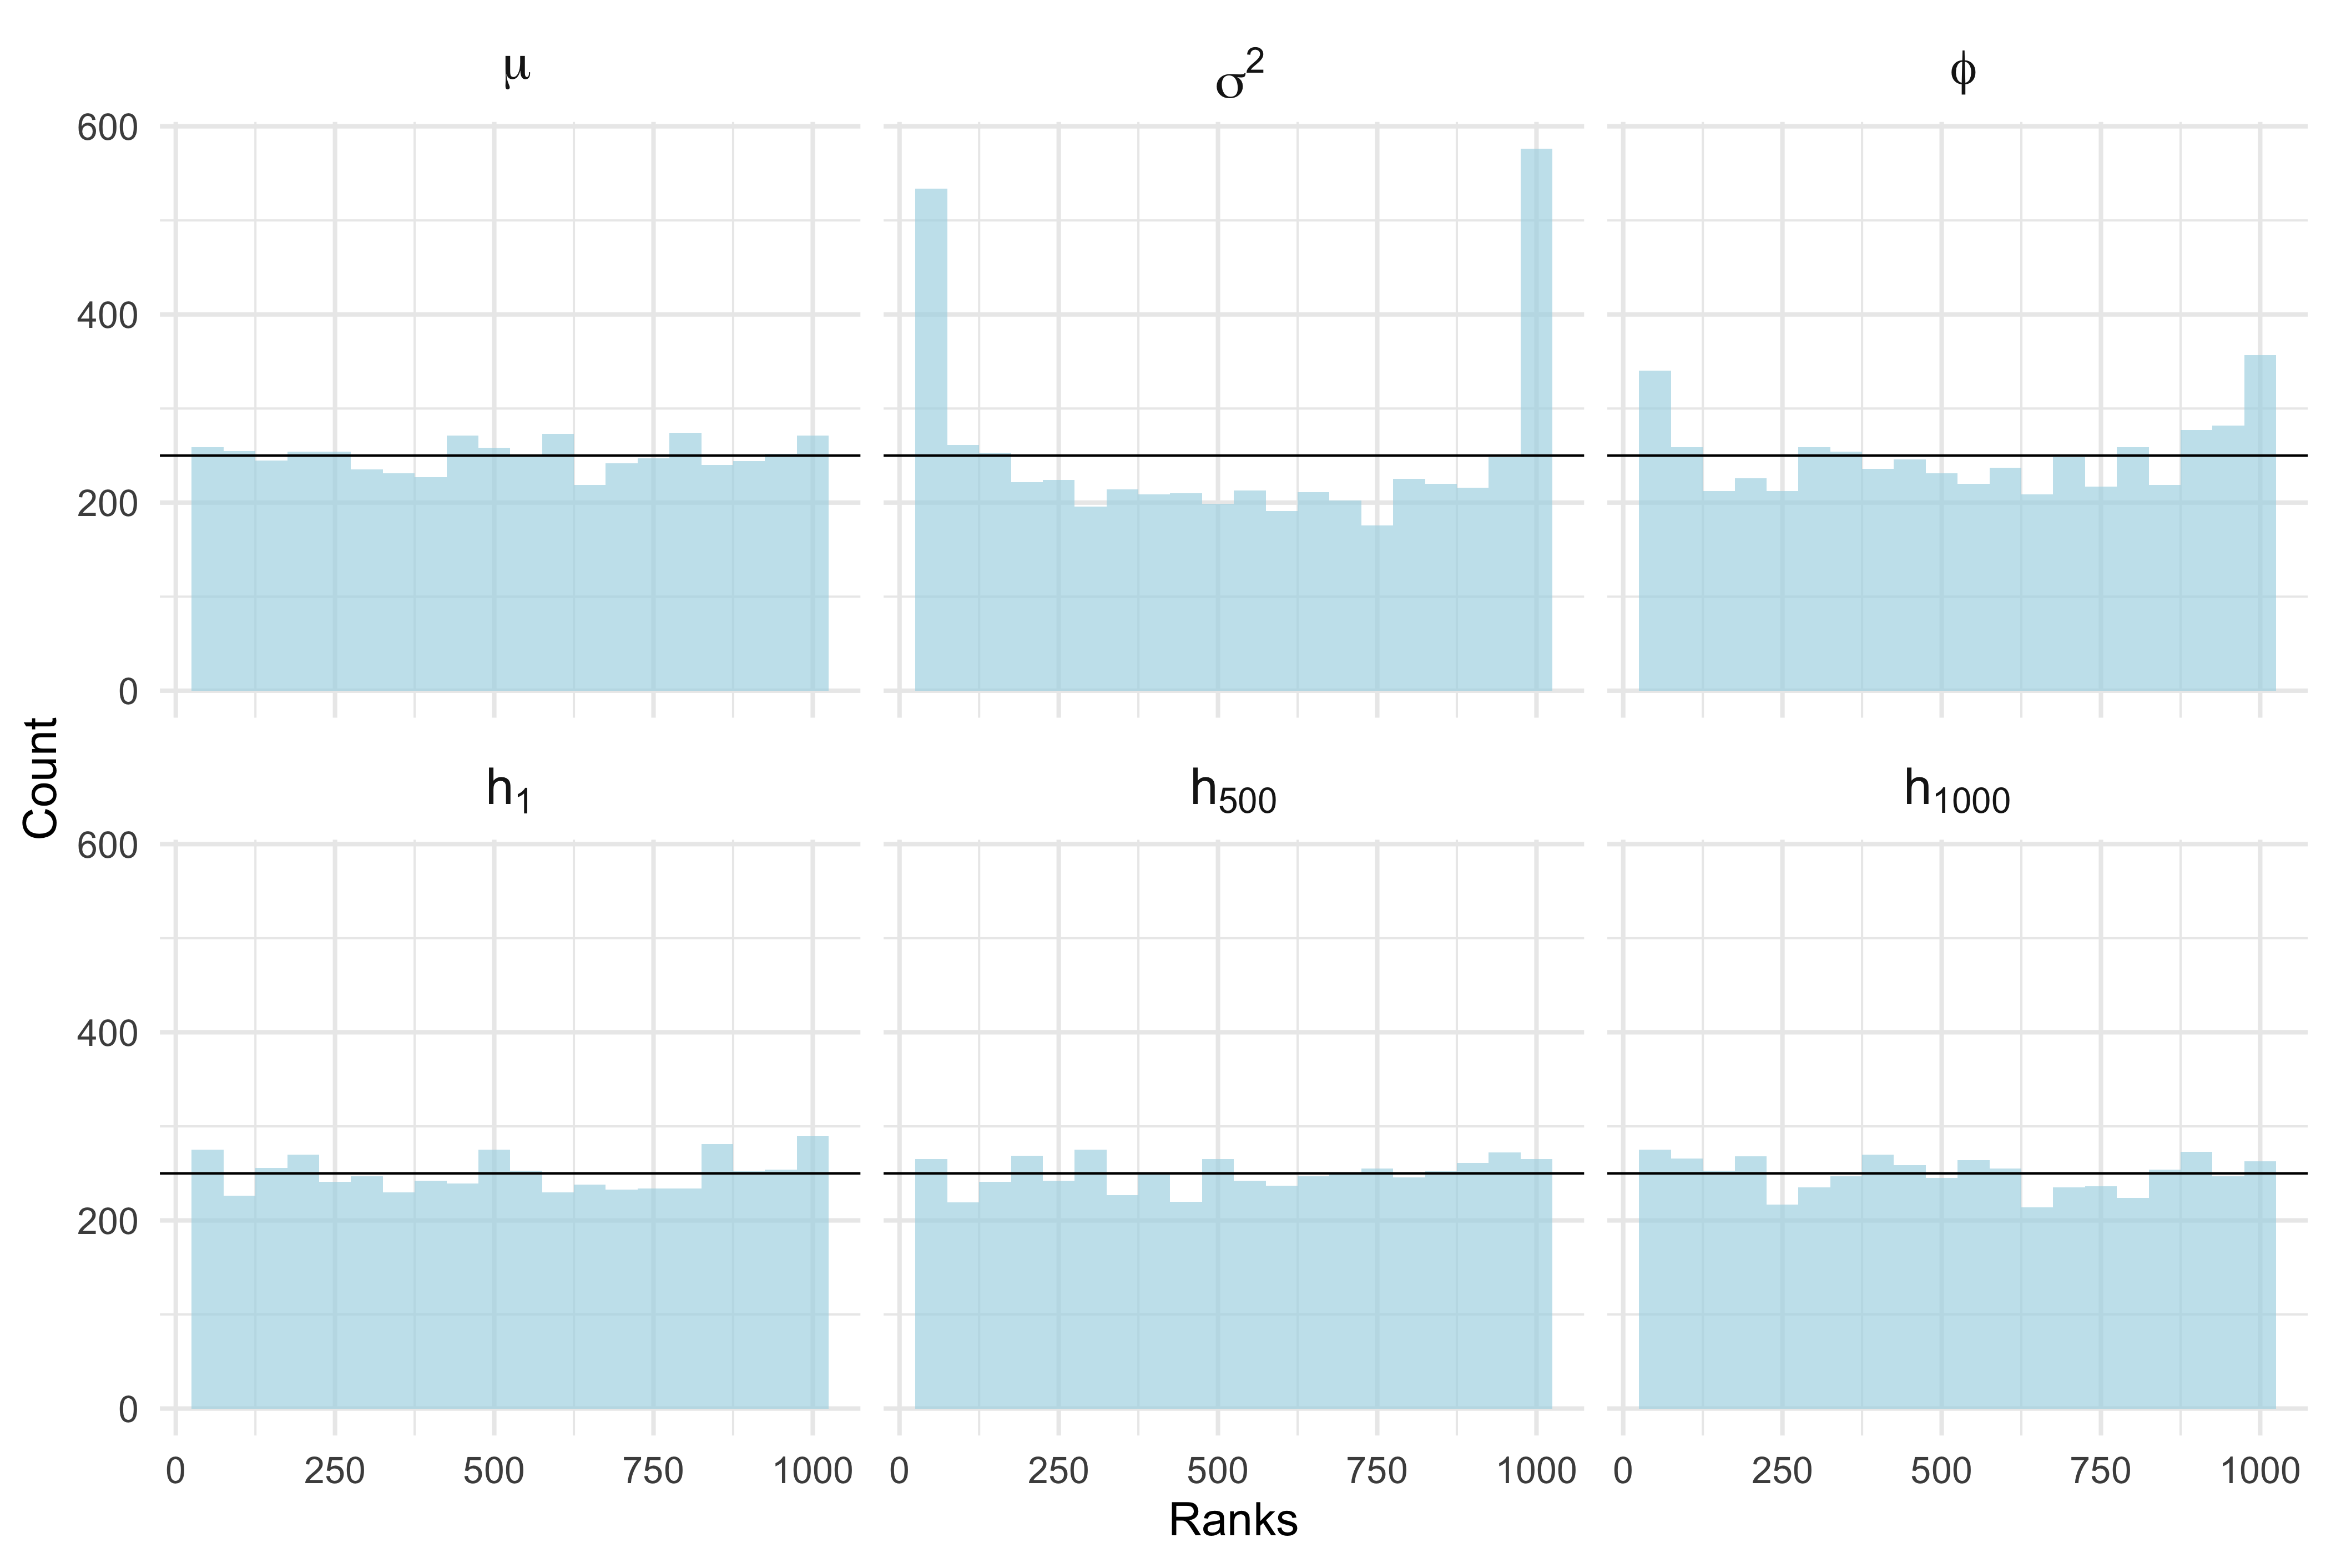
\includegraphics[scale=0.09]{results/hmc_cp_5k.png}
        \caption{5000 SBC iterations for centered model using Hamiltonian Monte Carlo. $\mu$ and the state parameters look approximately uniform. $\sigma^2$ still has major peaks on both the left and right hand side indicating under-dispersion relative to the prior distribution. $\phi$ exhibits a similar shape to $\sigma^2$ although the peaks are much smaller.}
        \label{fig:cphmc5k}
    \end{figure}

    \begin{figure}[H]
        \centering
        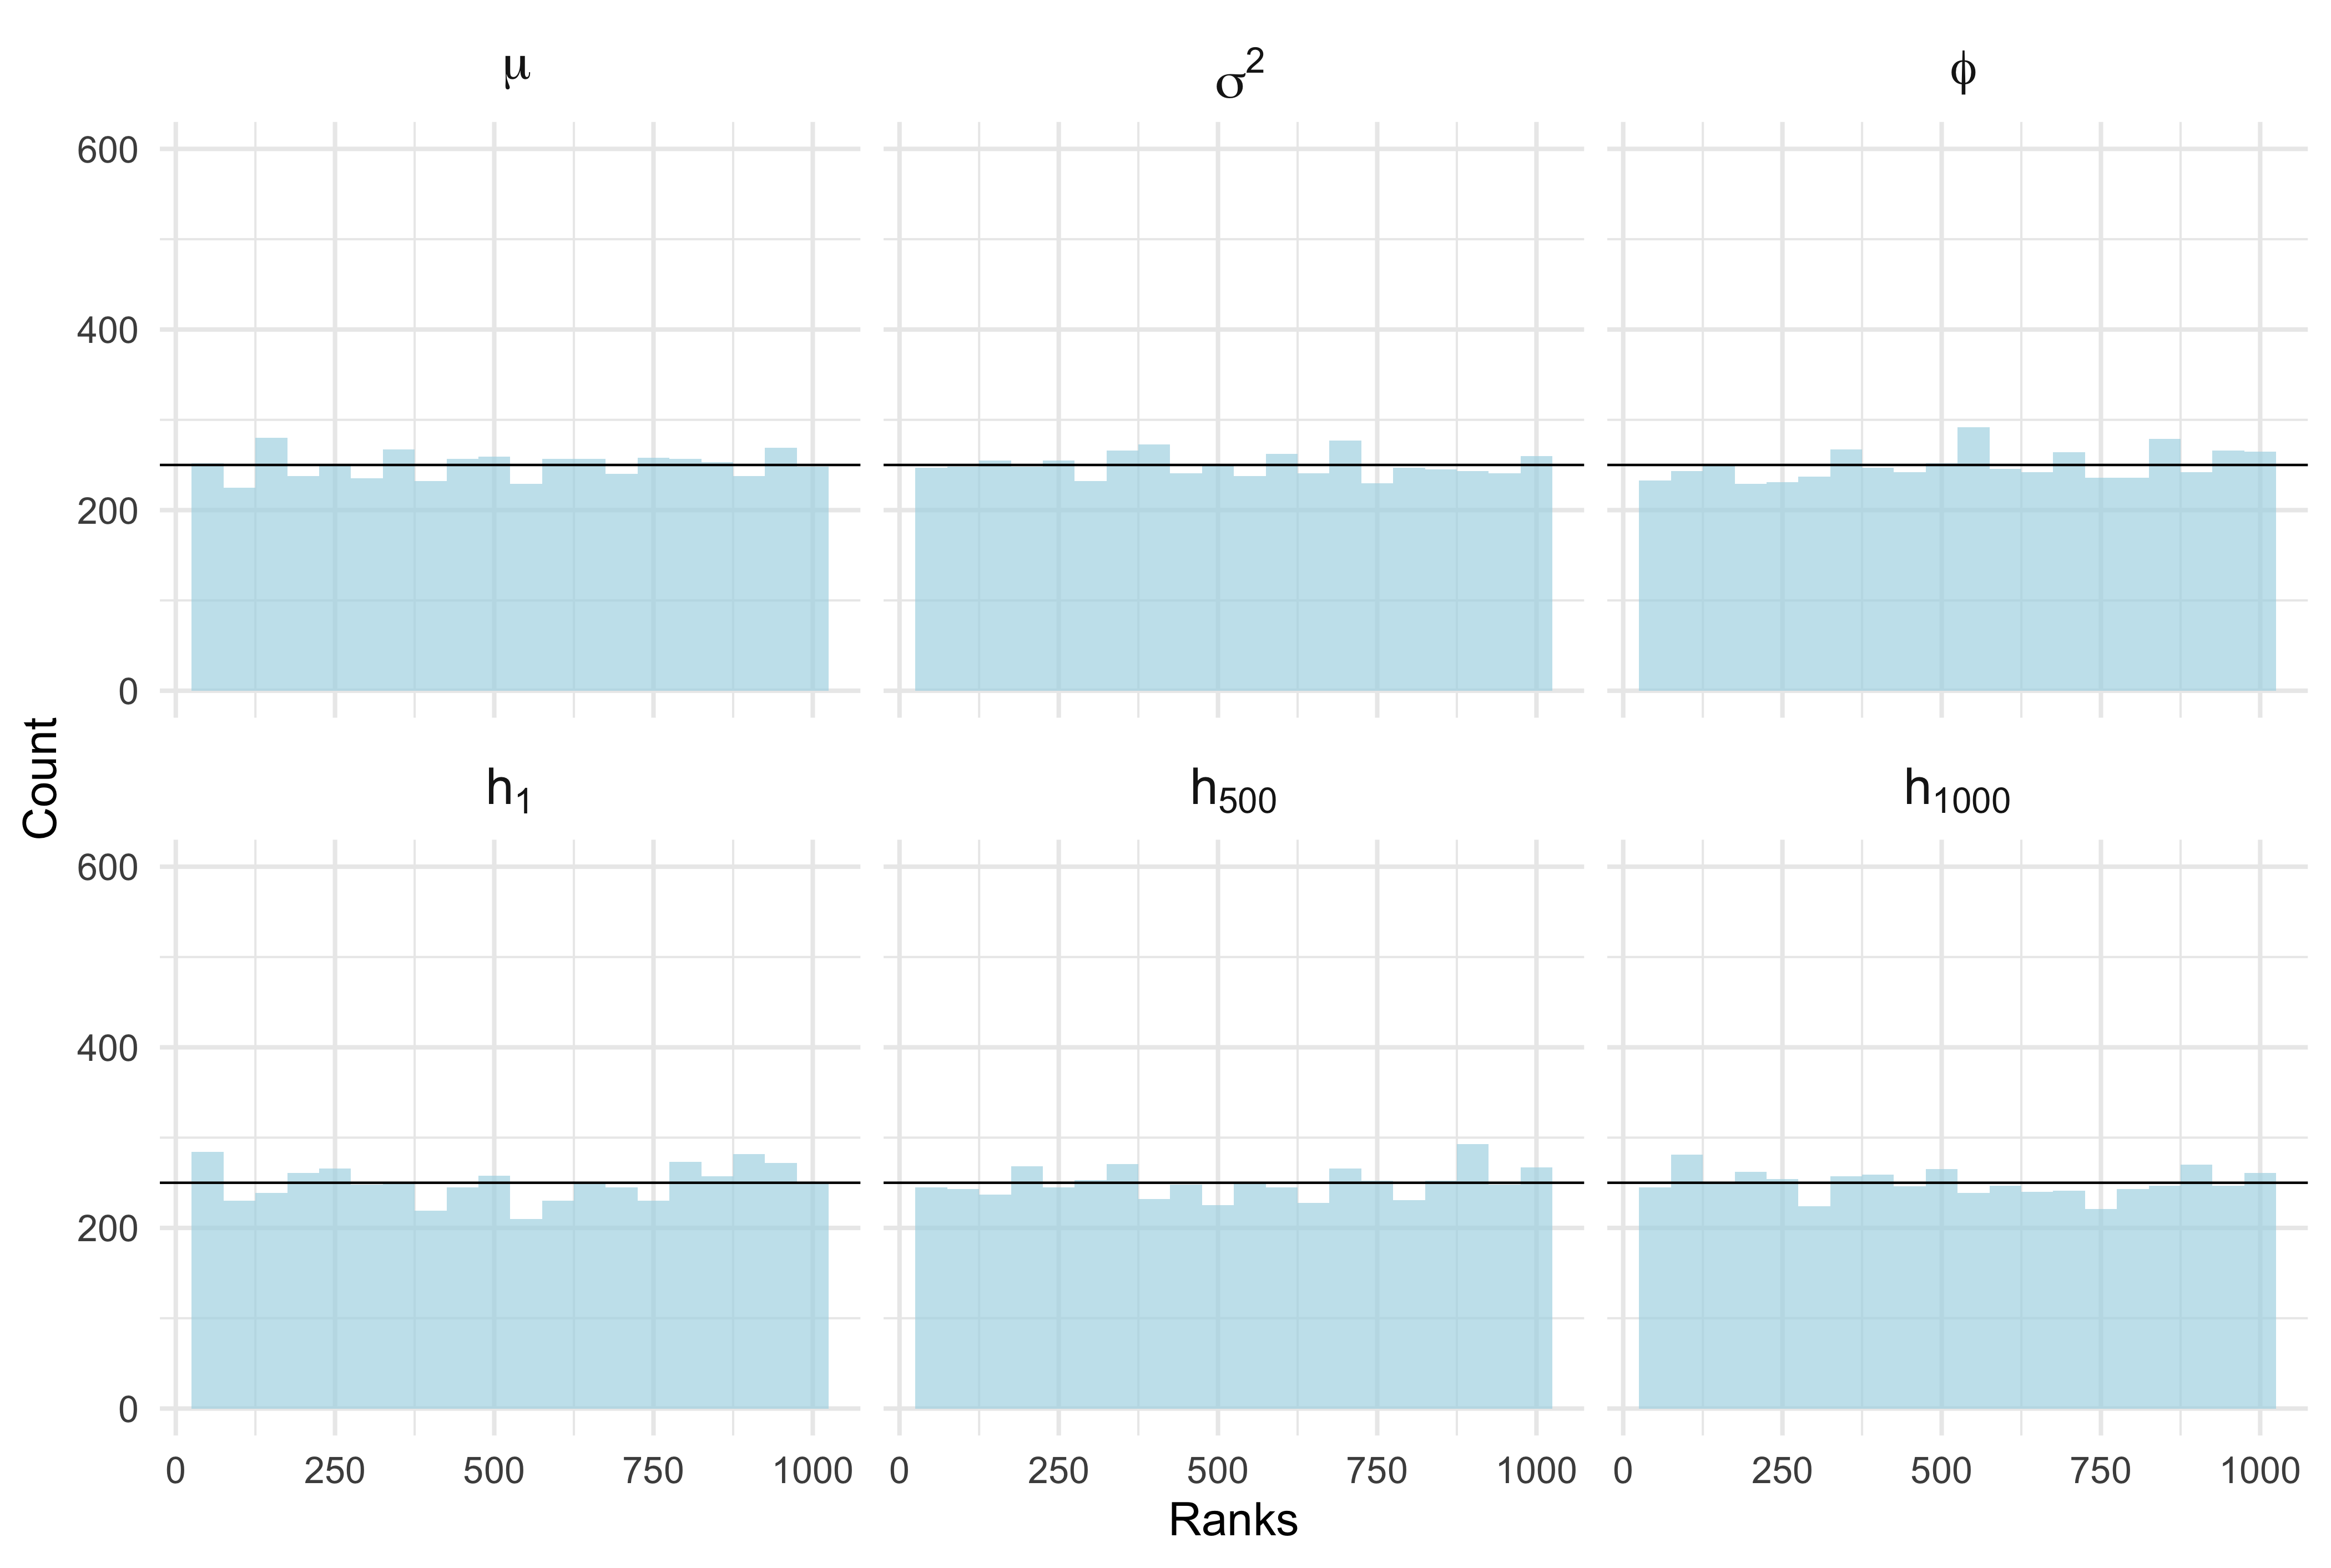
\includegraphics[scale=0.09]{results/hmc_ncp_5k.png}
        \caption{5000 SBC iterations for re-parameterised model using Hamiltonian Monte Carlo. Parameters display uniformity with less noise around the true uniform value. This suggests that the HMC algorithm is returning the correct posterior estimates for the selected parameters.}
        \label{fig:ncphmc5k}
    \end{figure}

    This computational difficulty in the centered parameterisation is reflected in the effective sample sizes. Figure \ref{fig:hmcess} and Table \ref{tab:hmcess} summarises the distribution of ESS for the static parameters after 5000 SBC iterations. The non centered model appears to generate independent samples much more efficiently than the centered model. This is consistent with HMC struggling to sample overall from the posteriors of $\sigma^2$ and $\phi$.

    \begin{figure}[H]
        \centering
        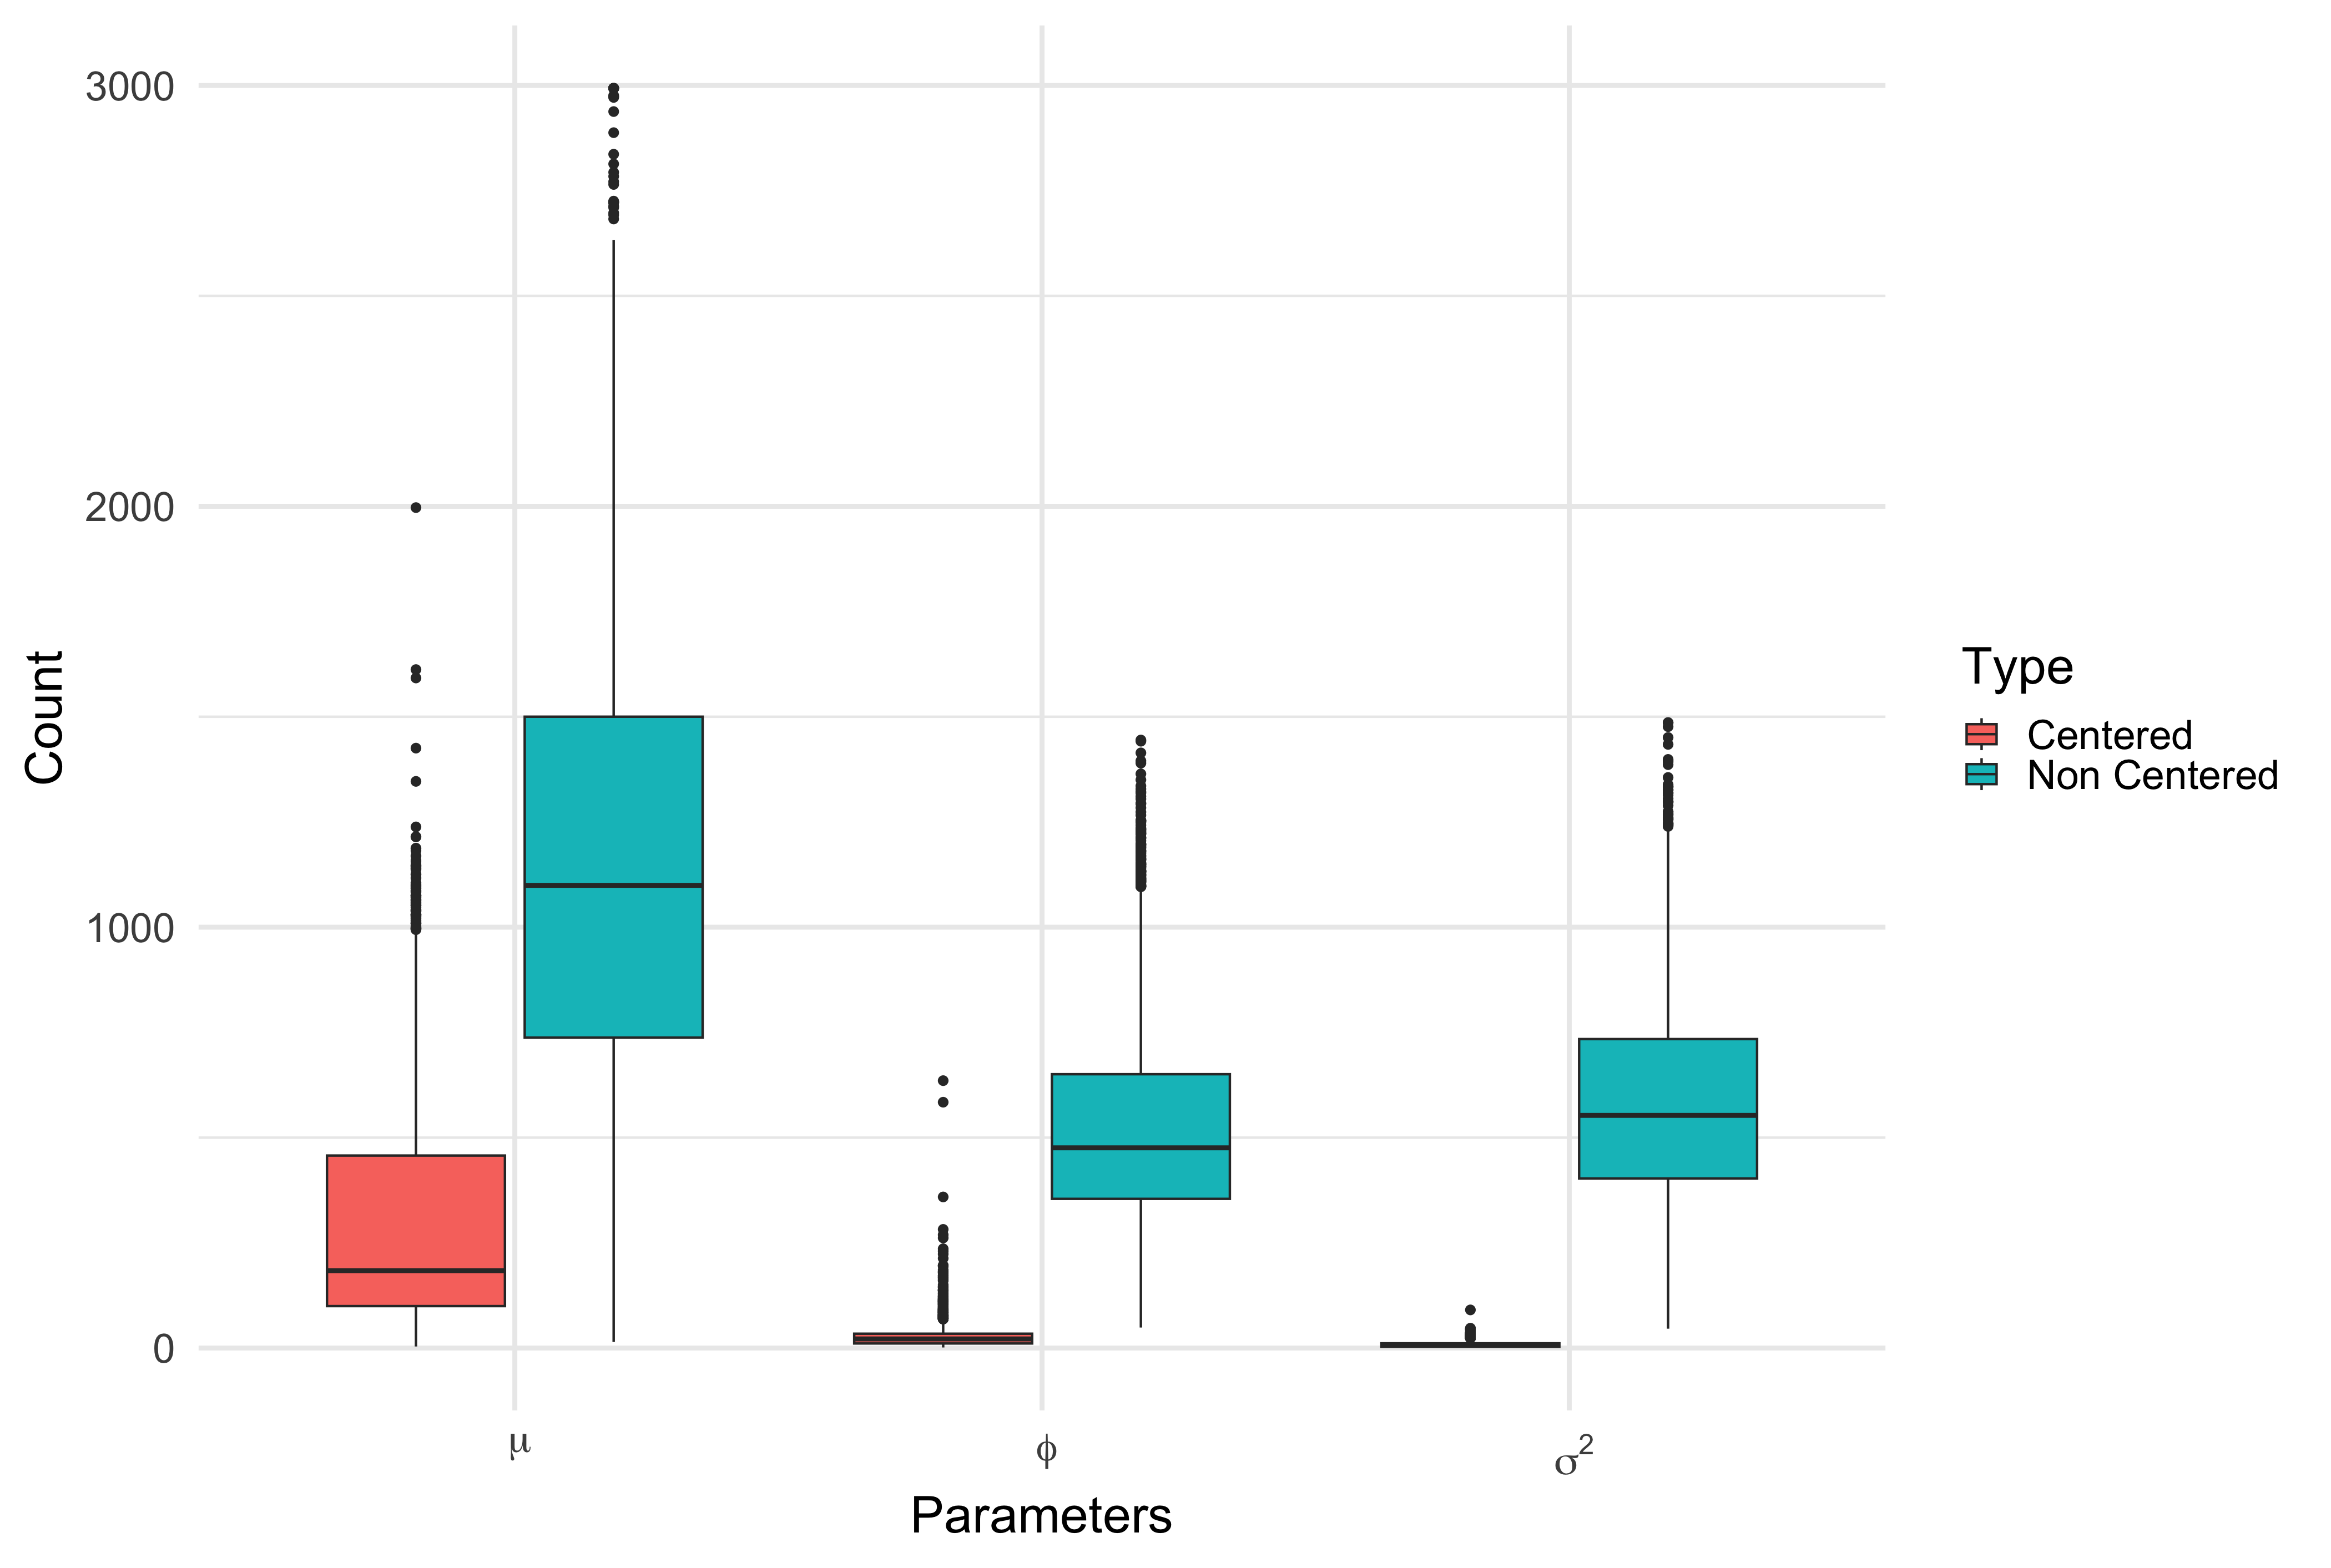
\includegraphics[scale=0.09]{results/hmc_ess.png}
        \caption{Effective sample sizes for static parameters after 5000 iterations of SBC and 1000 post warm-up samples for Hamiltonian Monte Carlo. The centered parameterisation struggles to generate independent samples for $\sigma^2$ and $\phi$. Non parameterisation demonstrates much more efficient sampling behaviour.}
        \label{fig:hmcess}
    \end{figure}

    \begin{table}[H]
        \centering
        \begin{tabular}{|c|c|c|c|c|c|c|c|} \hline 
        Parameter &  Type&Min& q25&  Median& Mean & q75&Max\\ \hline 
        $\mu$&  Centered&3.79 & 99.7 & 184. & 305. & 457. & 1997.  \\
     $\mu$&  Reparam&14.5 & 738. & 1099. & 1143. & 1500. & 2993.  \\\hline 
     $\phi$&  Centered&1.44 & 11.0 & 21.7 & 26.3 & 34.1 & 635.  \\
     $\phi$&  Reparam&48.8 & 355. & 476. & 521. & 651. & 1445.   \\ \hline 
     $\sigma^2$&  Centered& 1.17 & 2.99 & 7.04 & 8.05 & 11.3 & 90.7 \\ 
     $\sigma^2$&  Reparam&46.1 & 403. & 553. & 585. & 734. & 1486. \\ \hline
        \end{tabular}
        \caption{ESS for centered and re-parameterised SV model across 5000 SBC iterations for HMC.}
        \label{tab:hmcess}
    \end{table}

    \subsection{Gaussian Mixture Approximation}
    The Gaussian Mixture Approximation is run with the first 10,000 samples discarded as burn-in (following the method of \citet{kim1998stochastic}). However, unlike KSC who take 750,000 posterior draws from the model, the number of posterior samples taken as part of the SBC procedure is 9,999. Taking 750,000 draws from the Gaussian mixture approximation would lead to issues due to disk space limitations and computational resources required to run SBC. Furthermore, the number of posterior samples is larger than the 999 taken for the SBC experiment run for Hamiltonian Monte Carlo. Earlier experiments attempted 999 post burn in draws for the Gaussian approximation, however there are concerns that such a short chain would not have converged onto the target posterior distribution. Therefore 9,999 draws was chosen as a compromise under both constraints. 

    The both the centered and re-parameterised Gaussian mixture model contains issues with calibration. Figure \ref{fig:cpksc1k} presents the results from the centered model. There is a lack of uniformity across all parameters. In particular, there is a large bias on the left hand side for $\mu$ and the 1st and 500th latent state variables. There is also a bias on the right hand hand side of $\phi$. This suggests overestimation and underestimation of the prior distribution respectively. $\sigma^2$ and the 1000th latent state don't appear to be uniform although this may be due to noisy estimates.

    \begin{figure}[H]
        \centering
        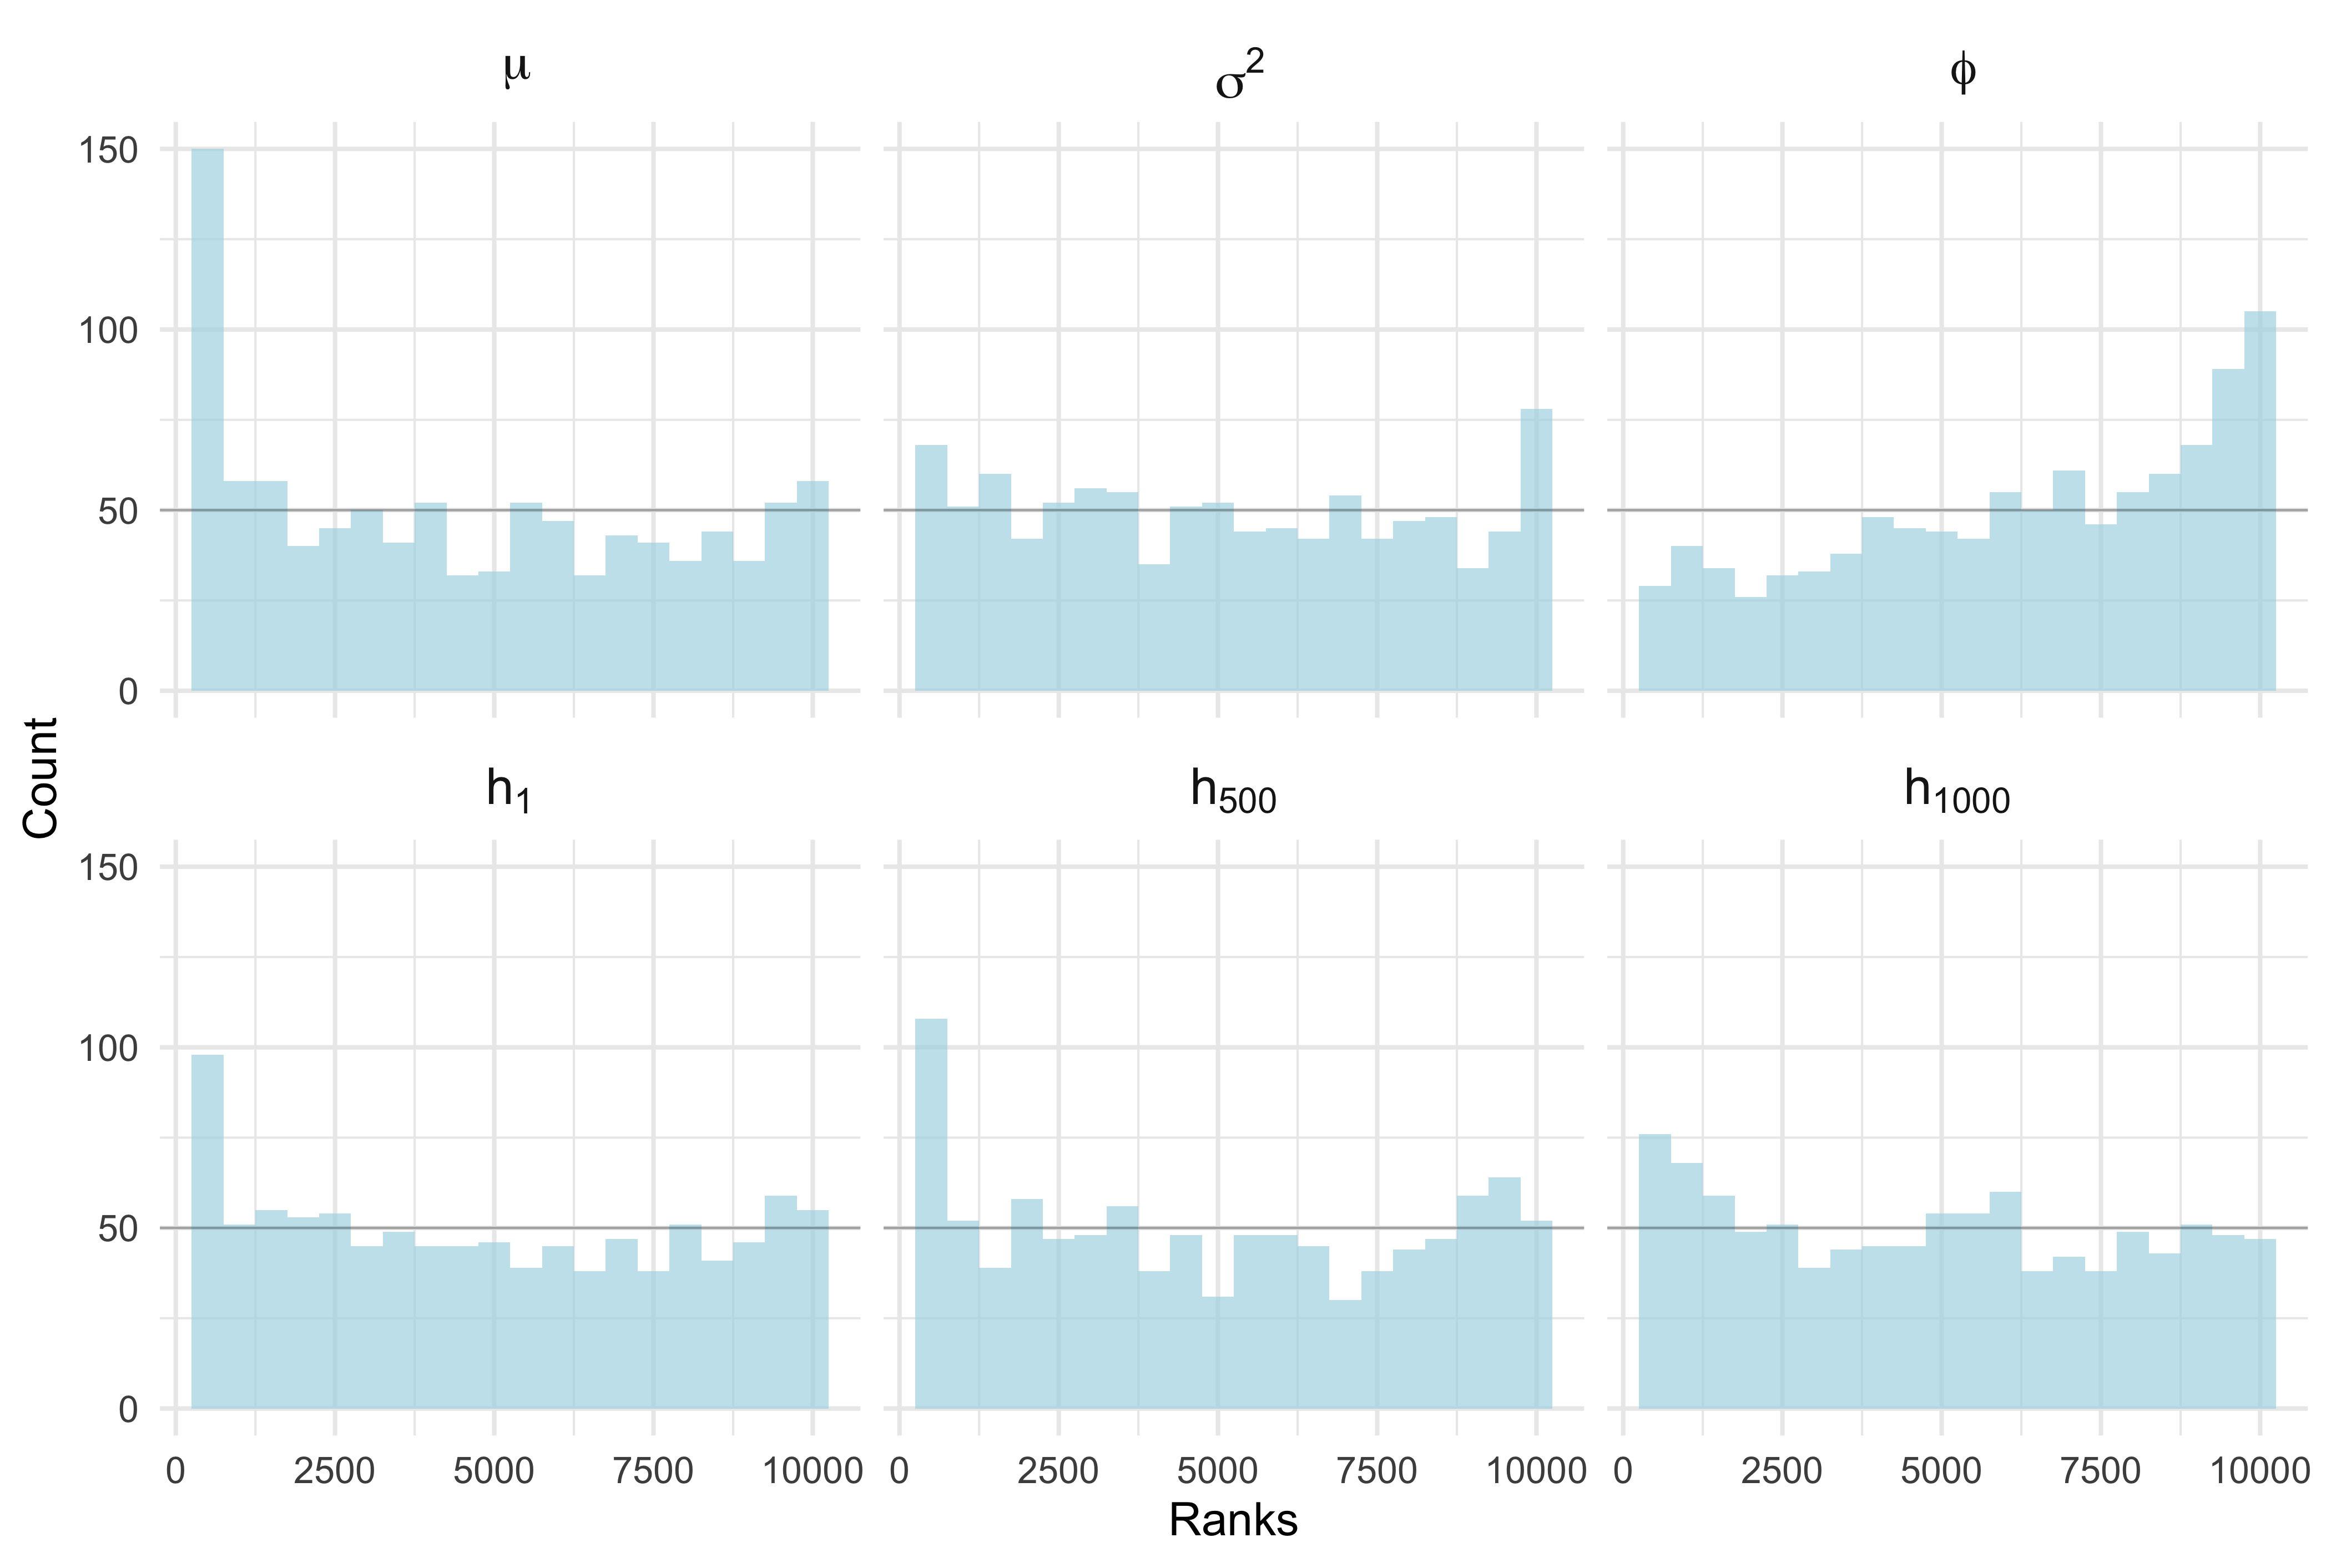
\includegraphics[scale=0.1]{results/ksc_cp_1k.png}
        \caption{1000 SBC iterations for centered Gaussian mixture approximation model. The rank statistics for all the selected parameters display a lack of uniformity. $\mu$ has a large left peak suggesting the algorithm is over estimating the true parameter. The converse can be said about $\phi$ which possesses a peak on the right hand side which implies underestimation of the true parameter. 1st and 500th latent state variables also appear to be over estimating the true value.}
        \label{fig:cpksc1k}
    \end{figure}

    The non centered model in location exhibits larger issues in calibration as shown in Figure \ref{fig:ncpksc1k}. Each histogram exhibits major peaks at one or both ends of the histgoram suggesting major issues in the sampler returning correct posterior estimates. The lack of uniformity for this model is distinctly due to a different shape. Whereas the lack of uniformity for some of the centered SBC results (for KSC) with 1000 iterations may be due to noisy estimates. 

    \begin{figure}[H]
        \centering
        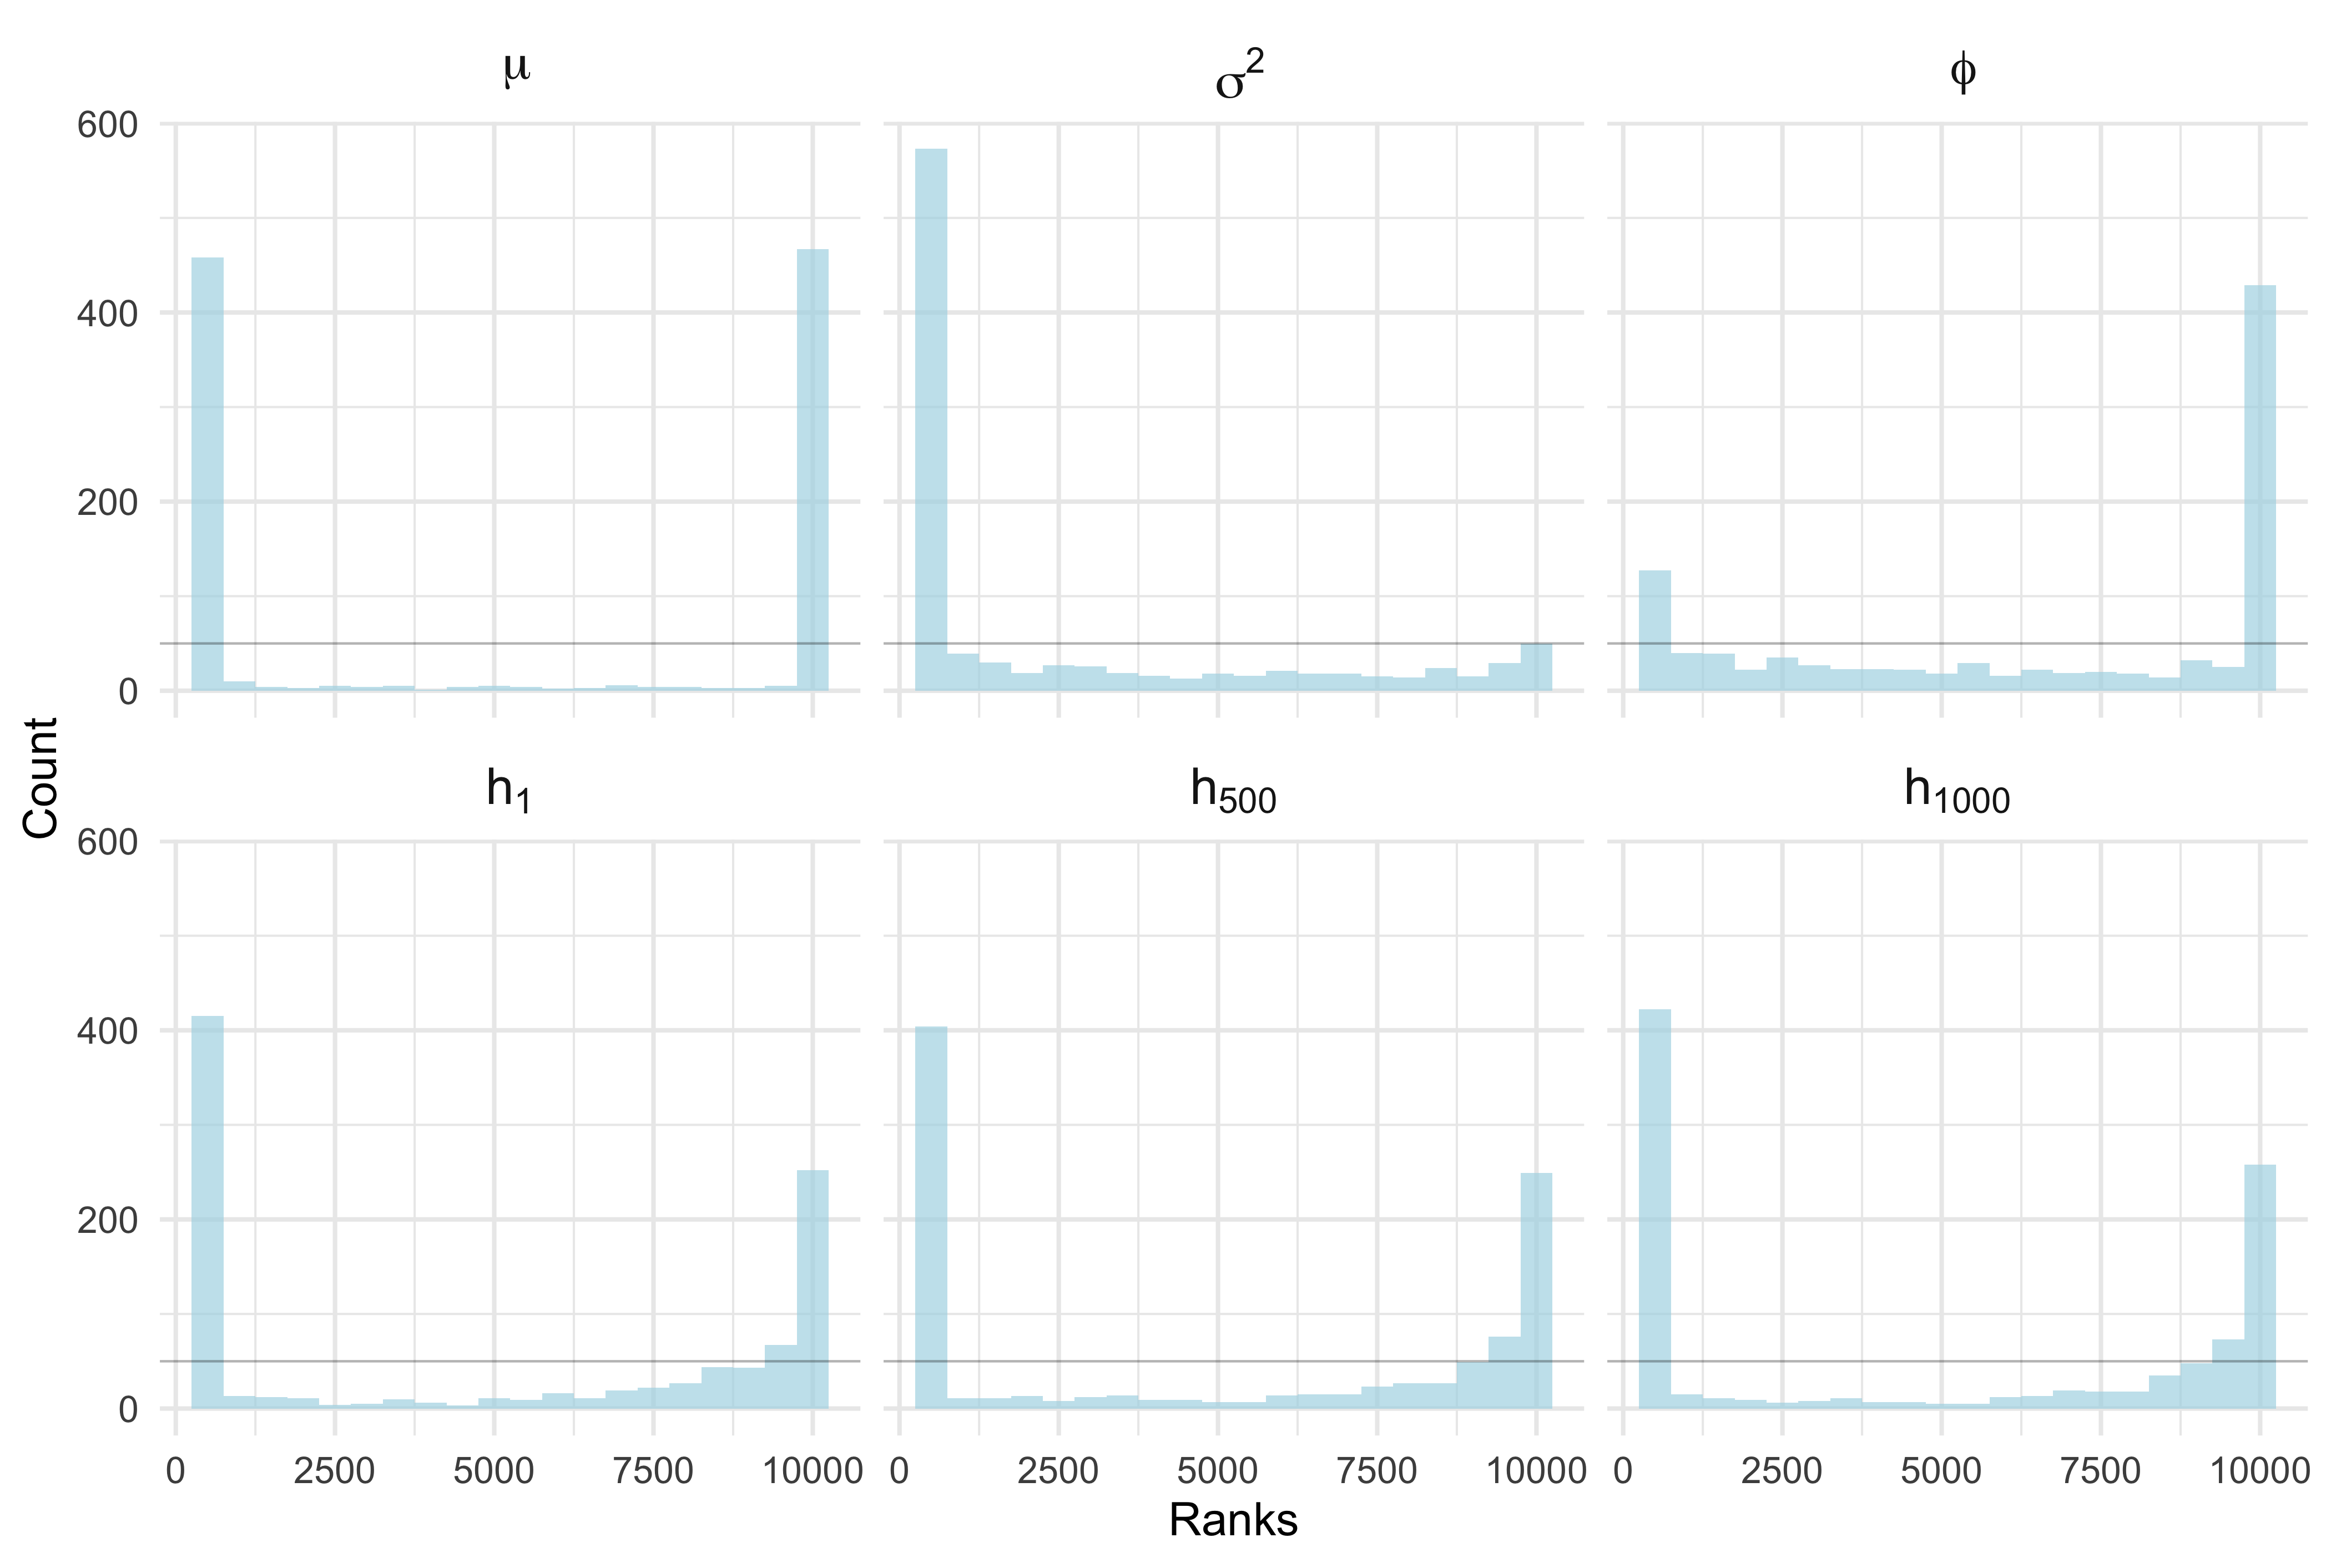
\includegraphics[scale=0.1]{results/ksc_ncp_1k.png}
        \caption{1000 SBC iterations for non centered in location Gaussian mixture approximation model. The rank statistics for all selected parameters are non uniform in shape. The KSC bespoke MCMC struggles to return the correct posteriors for this parameterisation of the model.}
        \label{fig:ncpksc1k}
    \end{figure}

    Increasing the SBC iterations to 5000 does not improve the results for either parameterisation. $\sigma^2$ contain arguably less noisy estimates around the uniform distribution in the centered parameterisation (although there may be evidence of a slight right bias). The skewed shapes of $\mu$ and $\phi$ adds further evidence that the sampling strategy is not returning the correct posterior estimates. All latent state variables appear to have a left side bias. This can be seen in Figure \ref{fig:cpksc5k}.

    Figure \ref{fig:ncpksc5k} shows no improvement to calibration results. The issues in calibration observed in Figure \ref{fig:ncpksc1k} are not due to noisy estimates and are likely the result of problems in the MCMC algorithm and model specification. Applying this parameterisation and MCMC on real data will on balance produce incorrect posterior estimates on average. 

    \begin{figure}[H]
        \centering
        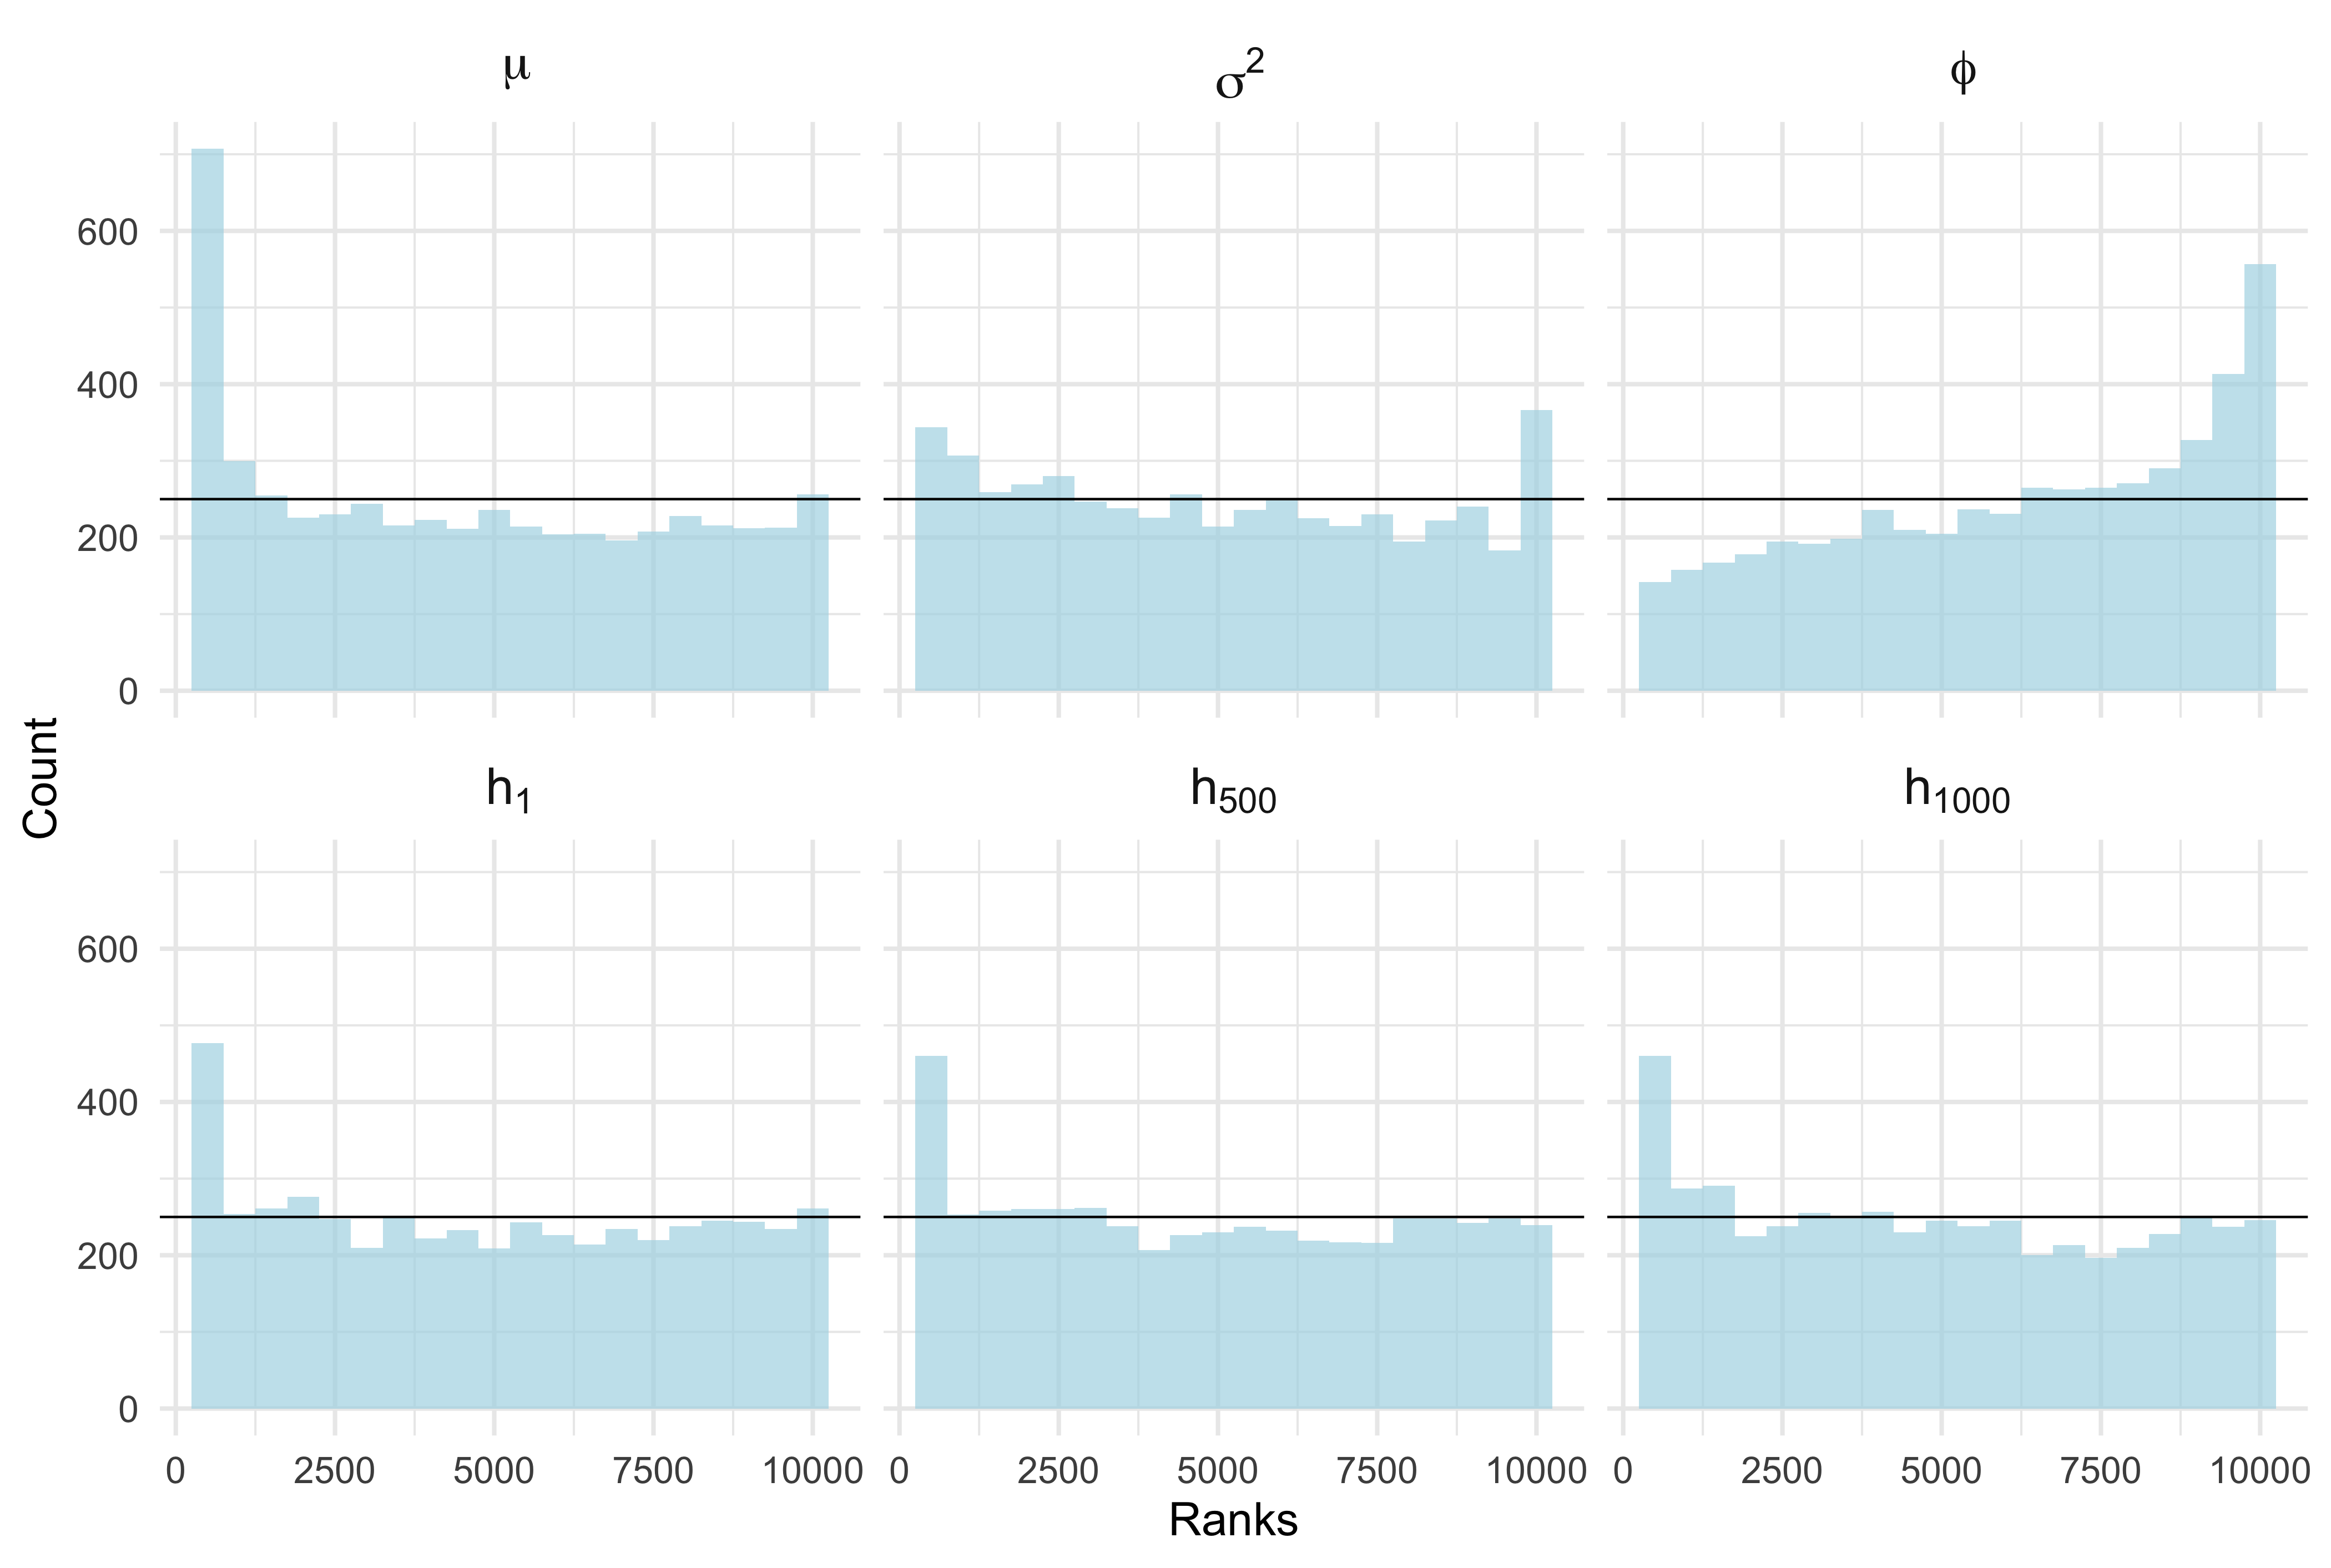
\includegraphics[scale=0.09]{results/ksc_cp_5k.png}
        \caption{5000 SBC iterations for centered Gaussian mixture approximation model. Estimates for $\sigma^2$ may have marginally improved around the uniformity there is still evidence of a ride side bias. There is no improvement in $\mu$ or $\phi$ and all latent state variables appear to have a left side bias.}
        \label{fig:cpksc5k}
    \end{figure}

    \begin{figure}[H]
        \centering
        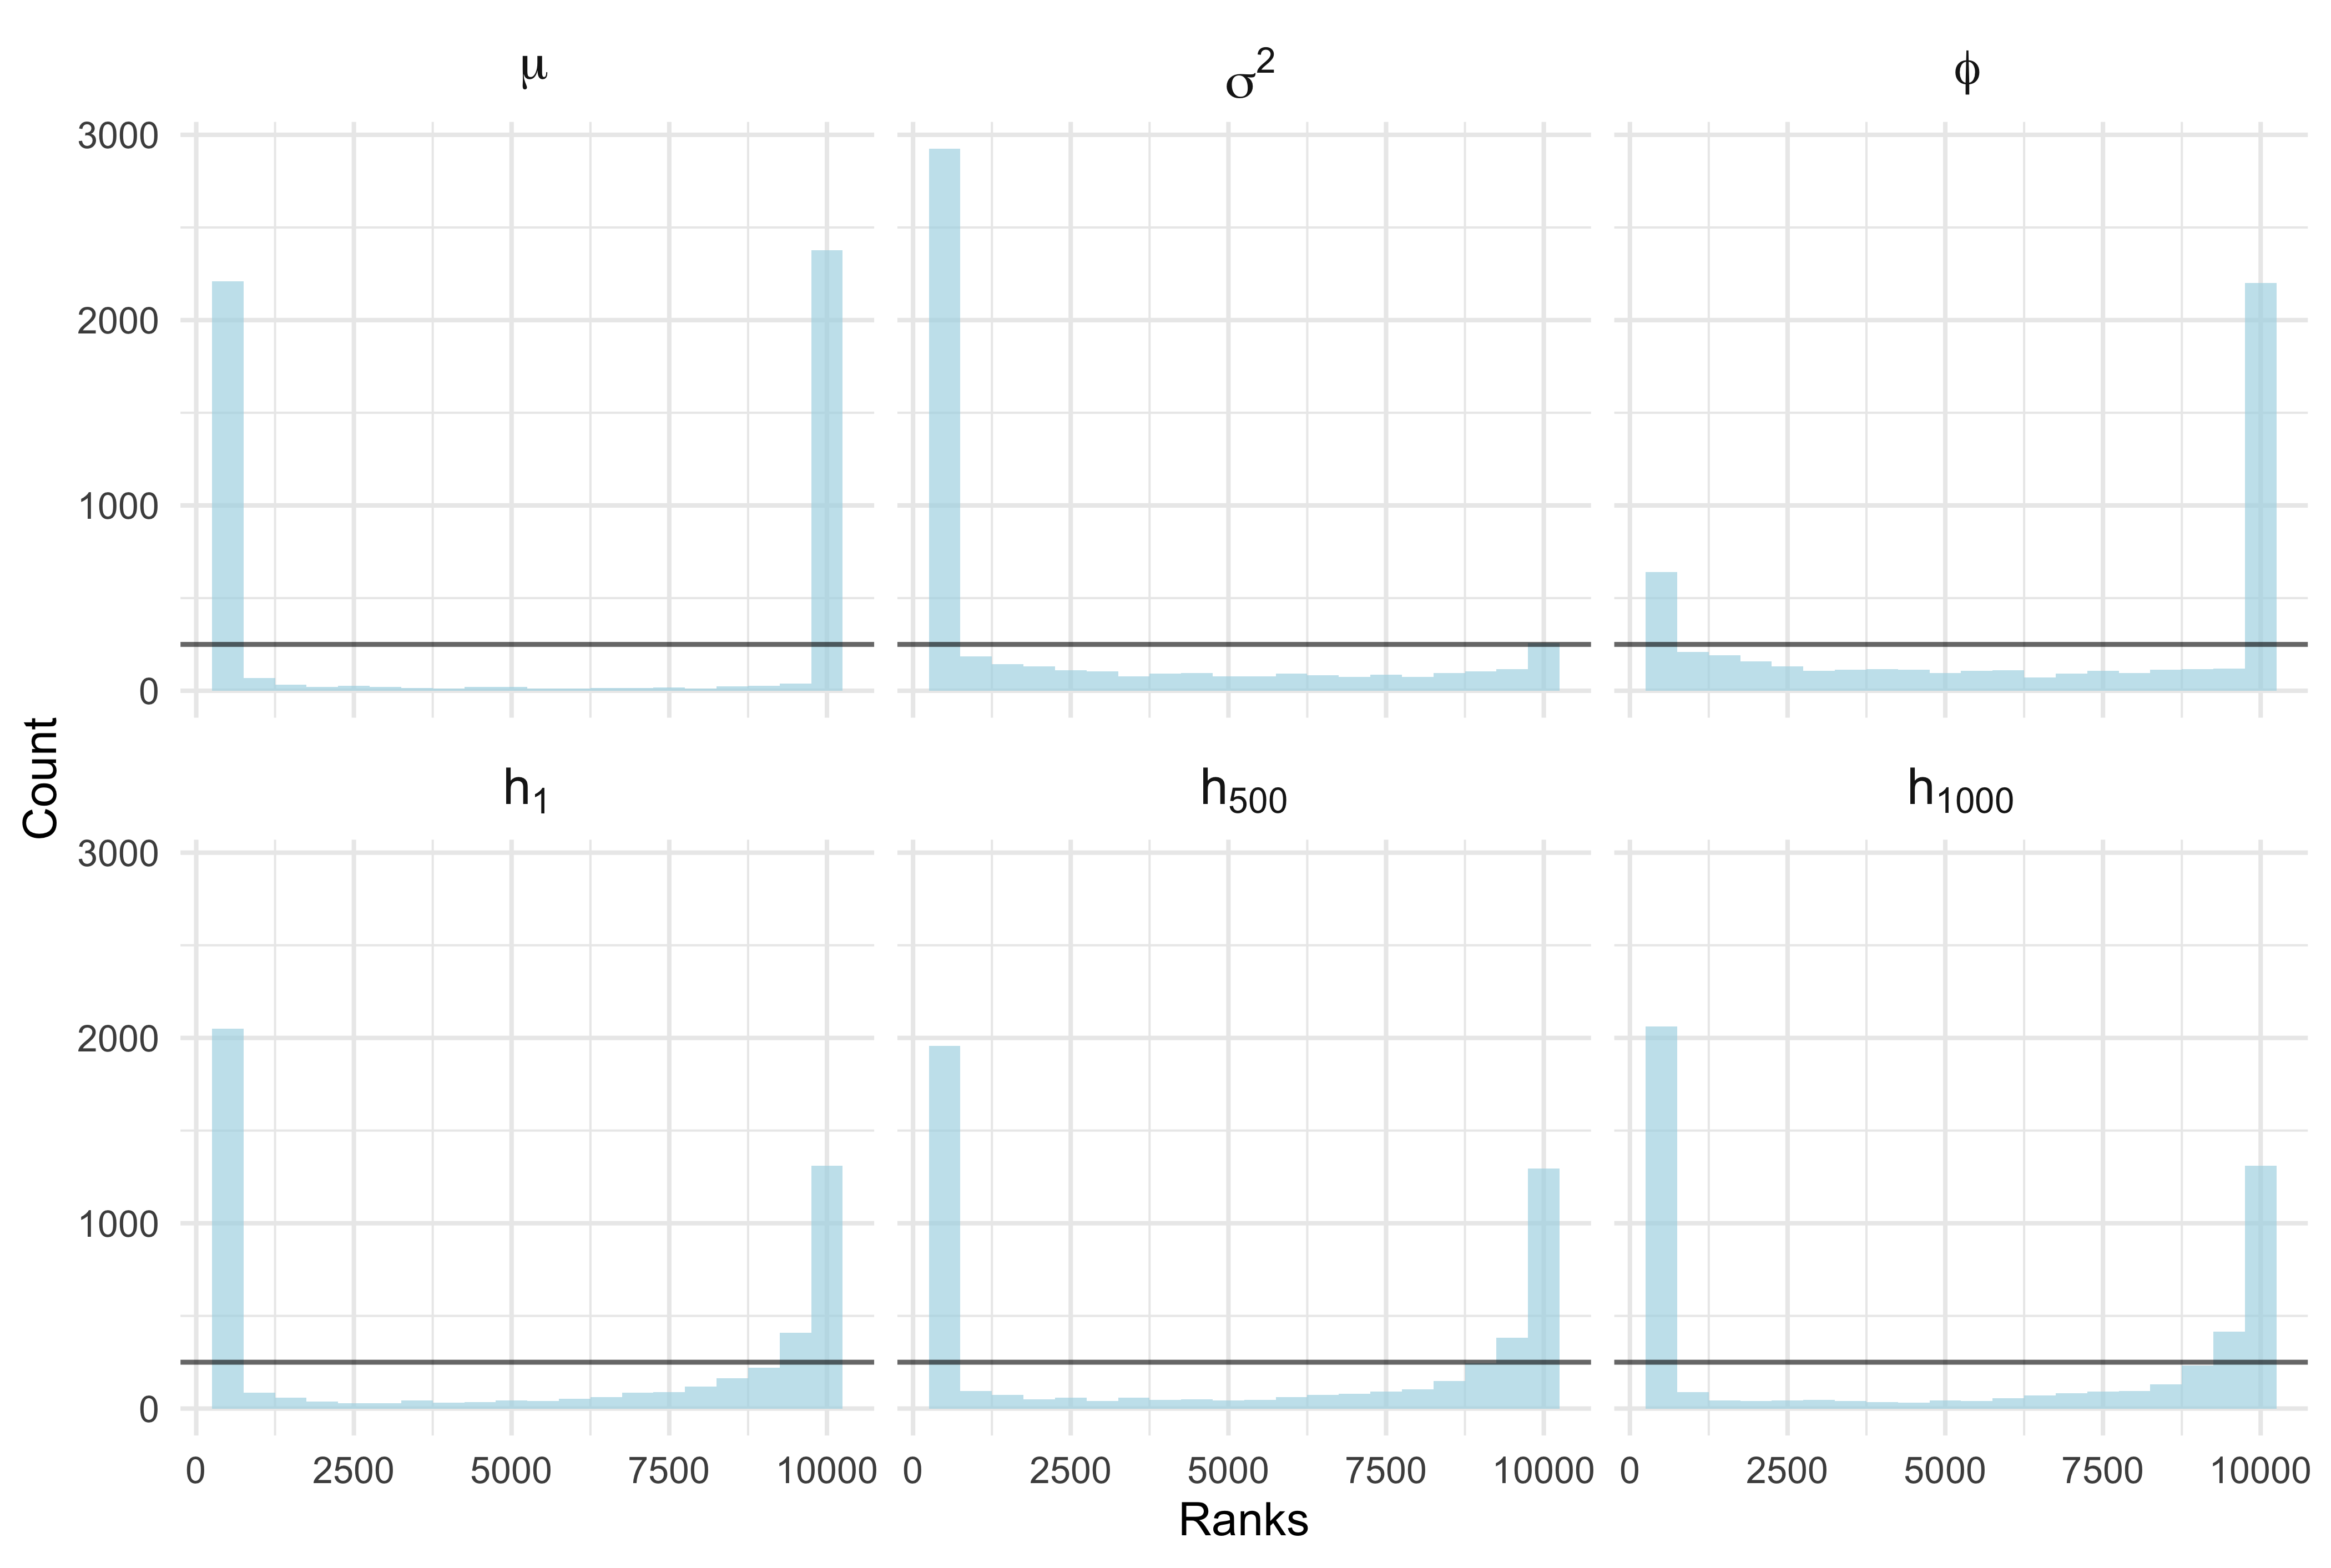
\includegraphics[scale=0.09]{results/ksc_ncp_5k.png}
        \caption{5000 SBC iterations for non centered Gaussian mixture approximation model. No improvement is observed in the distribution of rank statistics. The MCMC returns un-calibrated posterior estimates for this parameterisation of the model.}
        \label{fig:ncpksc5k}
    \end{figure}

    The ESS estimates for this model indicate a high degree of auto-correlation and difficulty in generating independent samples from both parameterisations. The numerical results are summarised in Figure \ref{fig:kscess} and Table \ref{tab:kscess}. The estimate for $\mu$ in the re-parameterised model exhibits a long right tail (longer than the 10,000 posterior draws suggesting the presence of negatively auto-correlated draws). There is some improvement in efficiency from the re-parameterised model with higher ESS values across most of the static parameter quantiles. Overall, the KSC bespoke MCMC is inefficient at sampling the static parameters. 
    
    % The median ESS for $\mu$, $\phi$ and $\sigma^2$ are 559, 103, 39.5 respectively for 10,000 post burn in draws. Despite having 10 times the number of draws, the number of effectively independent samples is much smaller relative to HMC, suggesting that this bespoke sampling strategy is highly inefficient. 

    % - reparam has massive long tail for mu

    \begin{figure}[H]
        \centering
        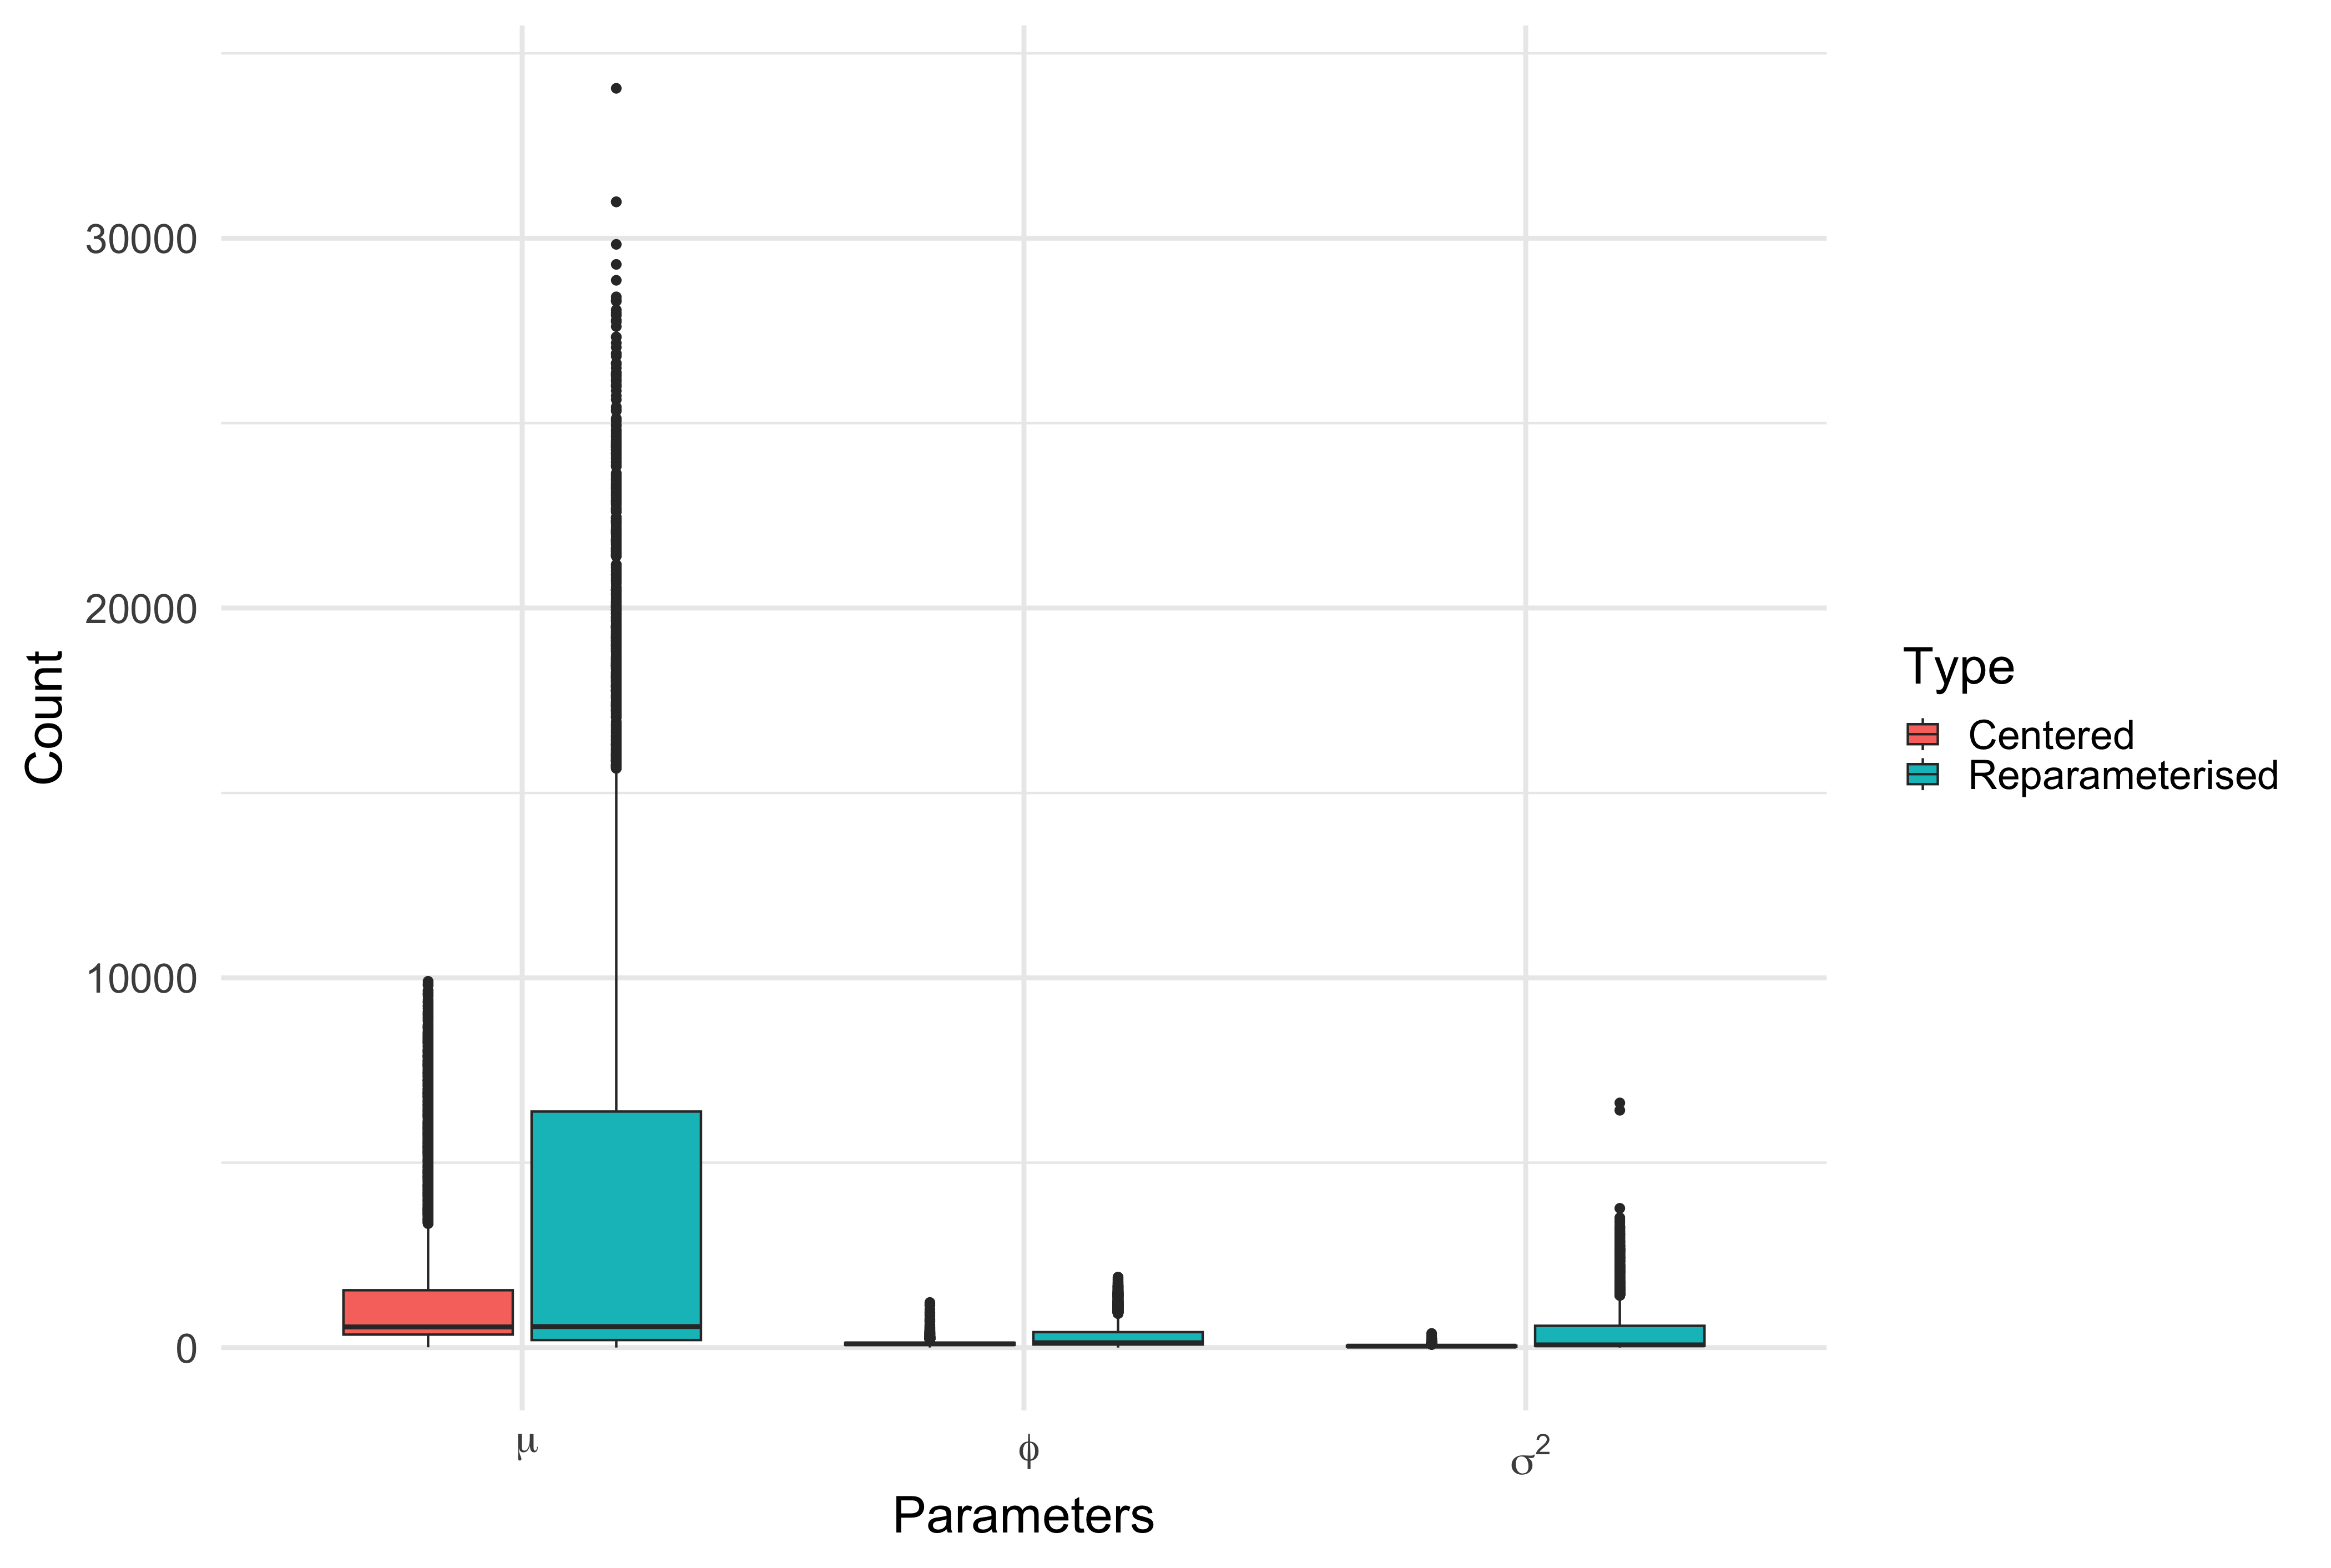
\includegraphics[scale=0.1]{results/ksc_ess.png}
        \caption{Effective sample sizes for static parameters after 5000 iterations of SBC and 1000 post burn-in samples for the Gaussian Mixture model. The bespoke sampling strategy struggles to generate independent samples for all static parameters, suggesting a high degree of auto-correlation in the Markov Chain.}
        \label{fig:kscess}
    \end{figure}

    \begin{table}[H]
        \centering
        \begin{tabular}{|c|c|c|c|c|c|c|c|} \hline 
        Parameter &  Type&Min& q25&  Median& Mean & q75&Max\\ \hline 
        $\mu$&  Centered&9.57 & 352. & 559. & 1482. & 1552. & 9907.\\
     $\mu$&  Reparam&1.99 & 205. & 569. & 4174. & 6384. & 34055.\\\hline 
     $\phi$&  Centered&2.47 & 74.0 & 103. & 112. & 130. & 1222.\\
     $\phi$&  Reparam&1.03 & 83.4 & 132. & 325. & 419. & 1907. \\ \hline 
     $\sigma^2$&  Centered&2.33 & 29.0 & 39.5 & 44.2 & 52.8 & 384. \\ 
     $\sigma^2$&  Reparam&1.25 & 47.4 & 73.4 & 399. & 591. & 6618. \\ \hline
        \end{tabular}
        \caption{KSC: ESS for centered and re-parameterised stochastic volatility model.}
        \label{tab:kscess}
    \end{table}

    The results from the KSC algorithm indicates issues with calibration. The centered parameterisation appears to be more favourable for this sampling approach. Other ways of improving the sampling of this model using this MCMC strategy could be to use another parameterisation such as non centered in scale.

    There are a few potential reasons for the poor calibration results. It may be due to the ineffectiveness of the MCMC strategy to generate the correct posteriors. Additionally, it could be due to the approximation of the actual stochastic volatility model not producing accurate posterior estimates. Correcting potential approximation error of the model is explored in the next section.  

    \subsection{Correcting approximation error using importance weights}
    \citet{kim1998stochastic} correct for approximation error in their method by using importance weights. The re-weighting procedure ensures that samples are drawn from the correct posterior density. This is applied to the calculation of the expected value of the stochastic volatility posterior density using samples drawn from the Gaussian mixture model. 

    Importance weights are defined as the ratio of the joint posterior from the stochastic volatility model and the posterior distribution of the approximate model. A weight is produced for each posterior sample generated by MCMC. These weights correct the samples from the approximate distribution by increasing or decreasing the contribution of that sample in the calculation of the expectation. 

    These weights can be applied in an additional sampling step using Metropolis Hastings or Importance Re-sampling (also known as sampling-importance re-sampling or SIR \citep{gelman2013bayesian}) to produce samples from the target posterior. However, the rank statistic can also be written as a function of the weighted expectation of the indicator random variable. This re-weighting step is applied to the calculation of the rank statistics to see if the correction improves the calibration of the MCMC sampler.\footnote{Efficiency estimates of the re-weighted posterior samples are omitted. It was unclear at the time of writing whether the ESS could be written as a function of the expectation or whether the ESS from re-sampled posterior samples using the importance weights are valid.}

    \subsubsection{Re-weighting rank statistics of the Gaussian Mixture Model}
    Let $v(\theta, h)$ be the log weights defined as the log difference between the posterior densities of the true model with log chi squared errors $log\: g(\theta, h | y^{\ast}_t)$ and the Gaussian mixture model $log\:  k(\theta, h_t | y^{\ast}_t)$.

    $$
    \begin{aligned}
        v(\theta, h) = log\: g(\theta, h | y^{\ast}_t) - log\:  k(\theta, h_t | y^{\ast}_t) = \text{const} + log\: g(y|h) - log\: k(y^{\ast} | h)
    \end{aligned}
    $$

    Take the exponential and normalise the weights for the $l^{th}$ posterior draw (note the constants cancel out):
    
    $$
    \begin{aligned}
    w^l = \frac{exp(v(\theta, h)_l)}{\sum_i exp(v(\theta, h)_i)}
    \end{aligned}
    $$

    This gives the normalised importance weight. The expectation for any function of the posterior samples can be written as a function of these weights. Let $S(\theta)$ be an indicator random variable that is a function of the posterior samples. The expectation can be written as:

    $$
    \begin{aligned}
    S(\theta) &= 1[\theta_l < \theta^{sim}] \\
    E[S(\theta) | y] &= \int s(\theta) g(\theta | y) d\theta\\ 
    &= \frac{\int s(\theta)\times exp(v(\theta, h)) * k(\theta, h_t | y^{\ast}_t)d\theta d h}{\int exp(v(\theta, h)) * k(\theta, h_t | y^{\ast}_t)d\theta d h} 
    \end{aligned}
    $$

    Therefore, the expectation of the re-weighted posterior samples is given by:

    $$
    \begin{aligned}
    E[S(\hat{\theta}) | y^{\ast}] = \sum_l^L S(\hat{\theta}_l)w_l
    \end{aligned}
    $$

    The rank statistic can be rewritten as a function of the expectation and weights. This gives us the re-weighted rank statistics.

    $$
    \begin{aligned}
    r = \sum_{l=1}^{L}1[\theta_{l} < \theta^{sim}] \approx  L\times E[S(\hat{\theta})] = L\times \sum_l^L S(\hat{\theta}_l)w_l
    \end{aligned}
    $$

    The results from applying this re-weighting step to the rank statistics of the centered model are given on Figure \ref{fig:reweight1k}. There are no improvements in the distribution of rank statistics. Increasing the SBC iterations to 5000 as seen in Figure \ref{fig:reweight5k} also show no major improvements. The shape of both sets of histograms is consistent with the shape of the unweighted rank statistics. Overall the re-weighting of the posterior samples from the approximate model does not improve the calibration results. The re-weighted rank statistics for the re-parameterised model also did not improve and can be found in Appendix D.

    \begin{figure}[H]
        \centering
        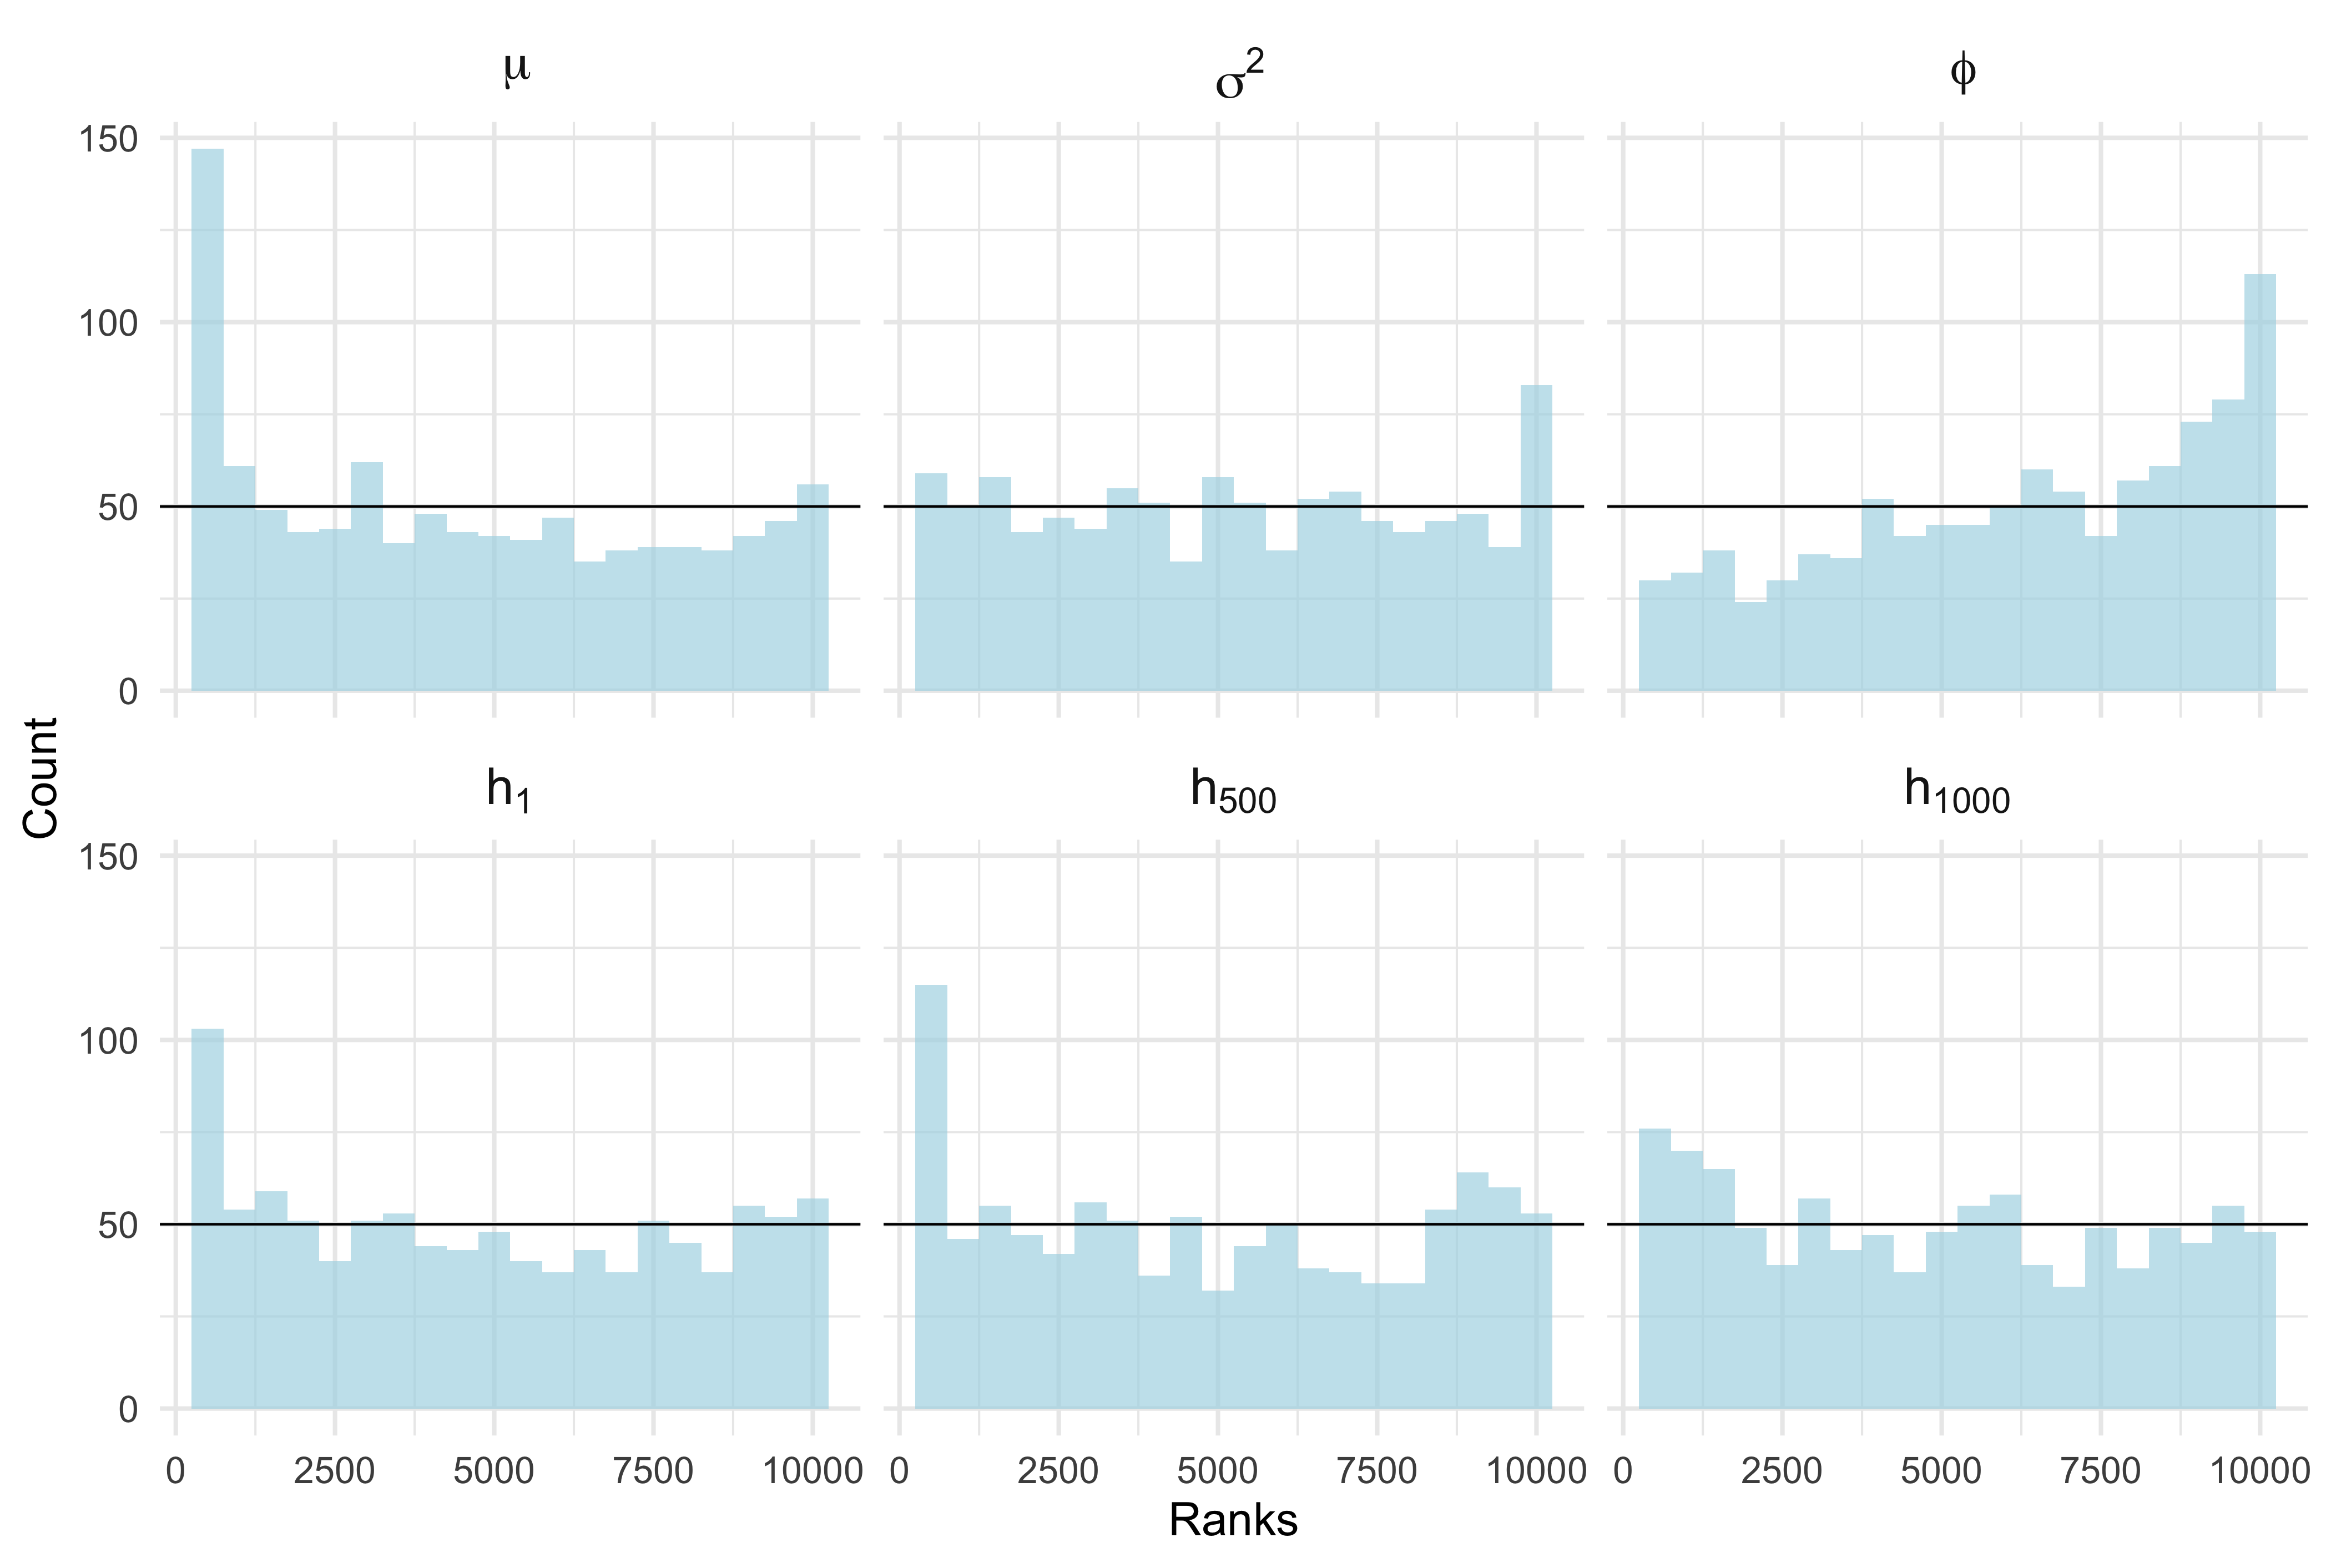
\includegraphics[scale=0.1]{results/weighted_ksc_cp_1k.png}
        \caption{1000 SBC iterations for re-weighted rank statistics from the Gaussian mixture approximation model. The shape of the histogram is consistent with the unweighted rank statistics.}
        \label{fig:reweight1k}
    \end{figure}

    \begin{figure}[H]
        \centering
        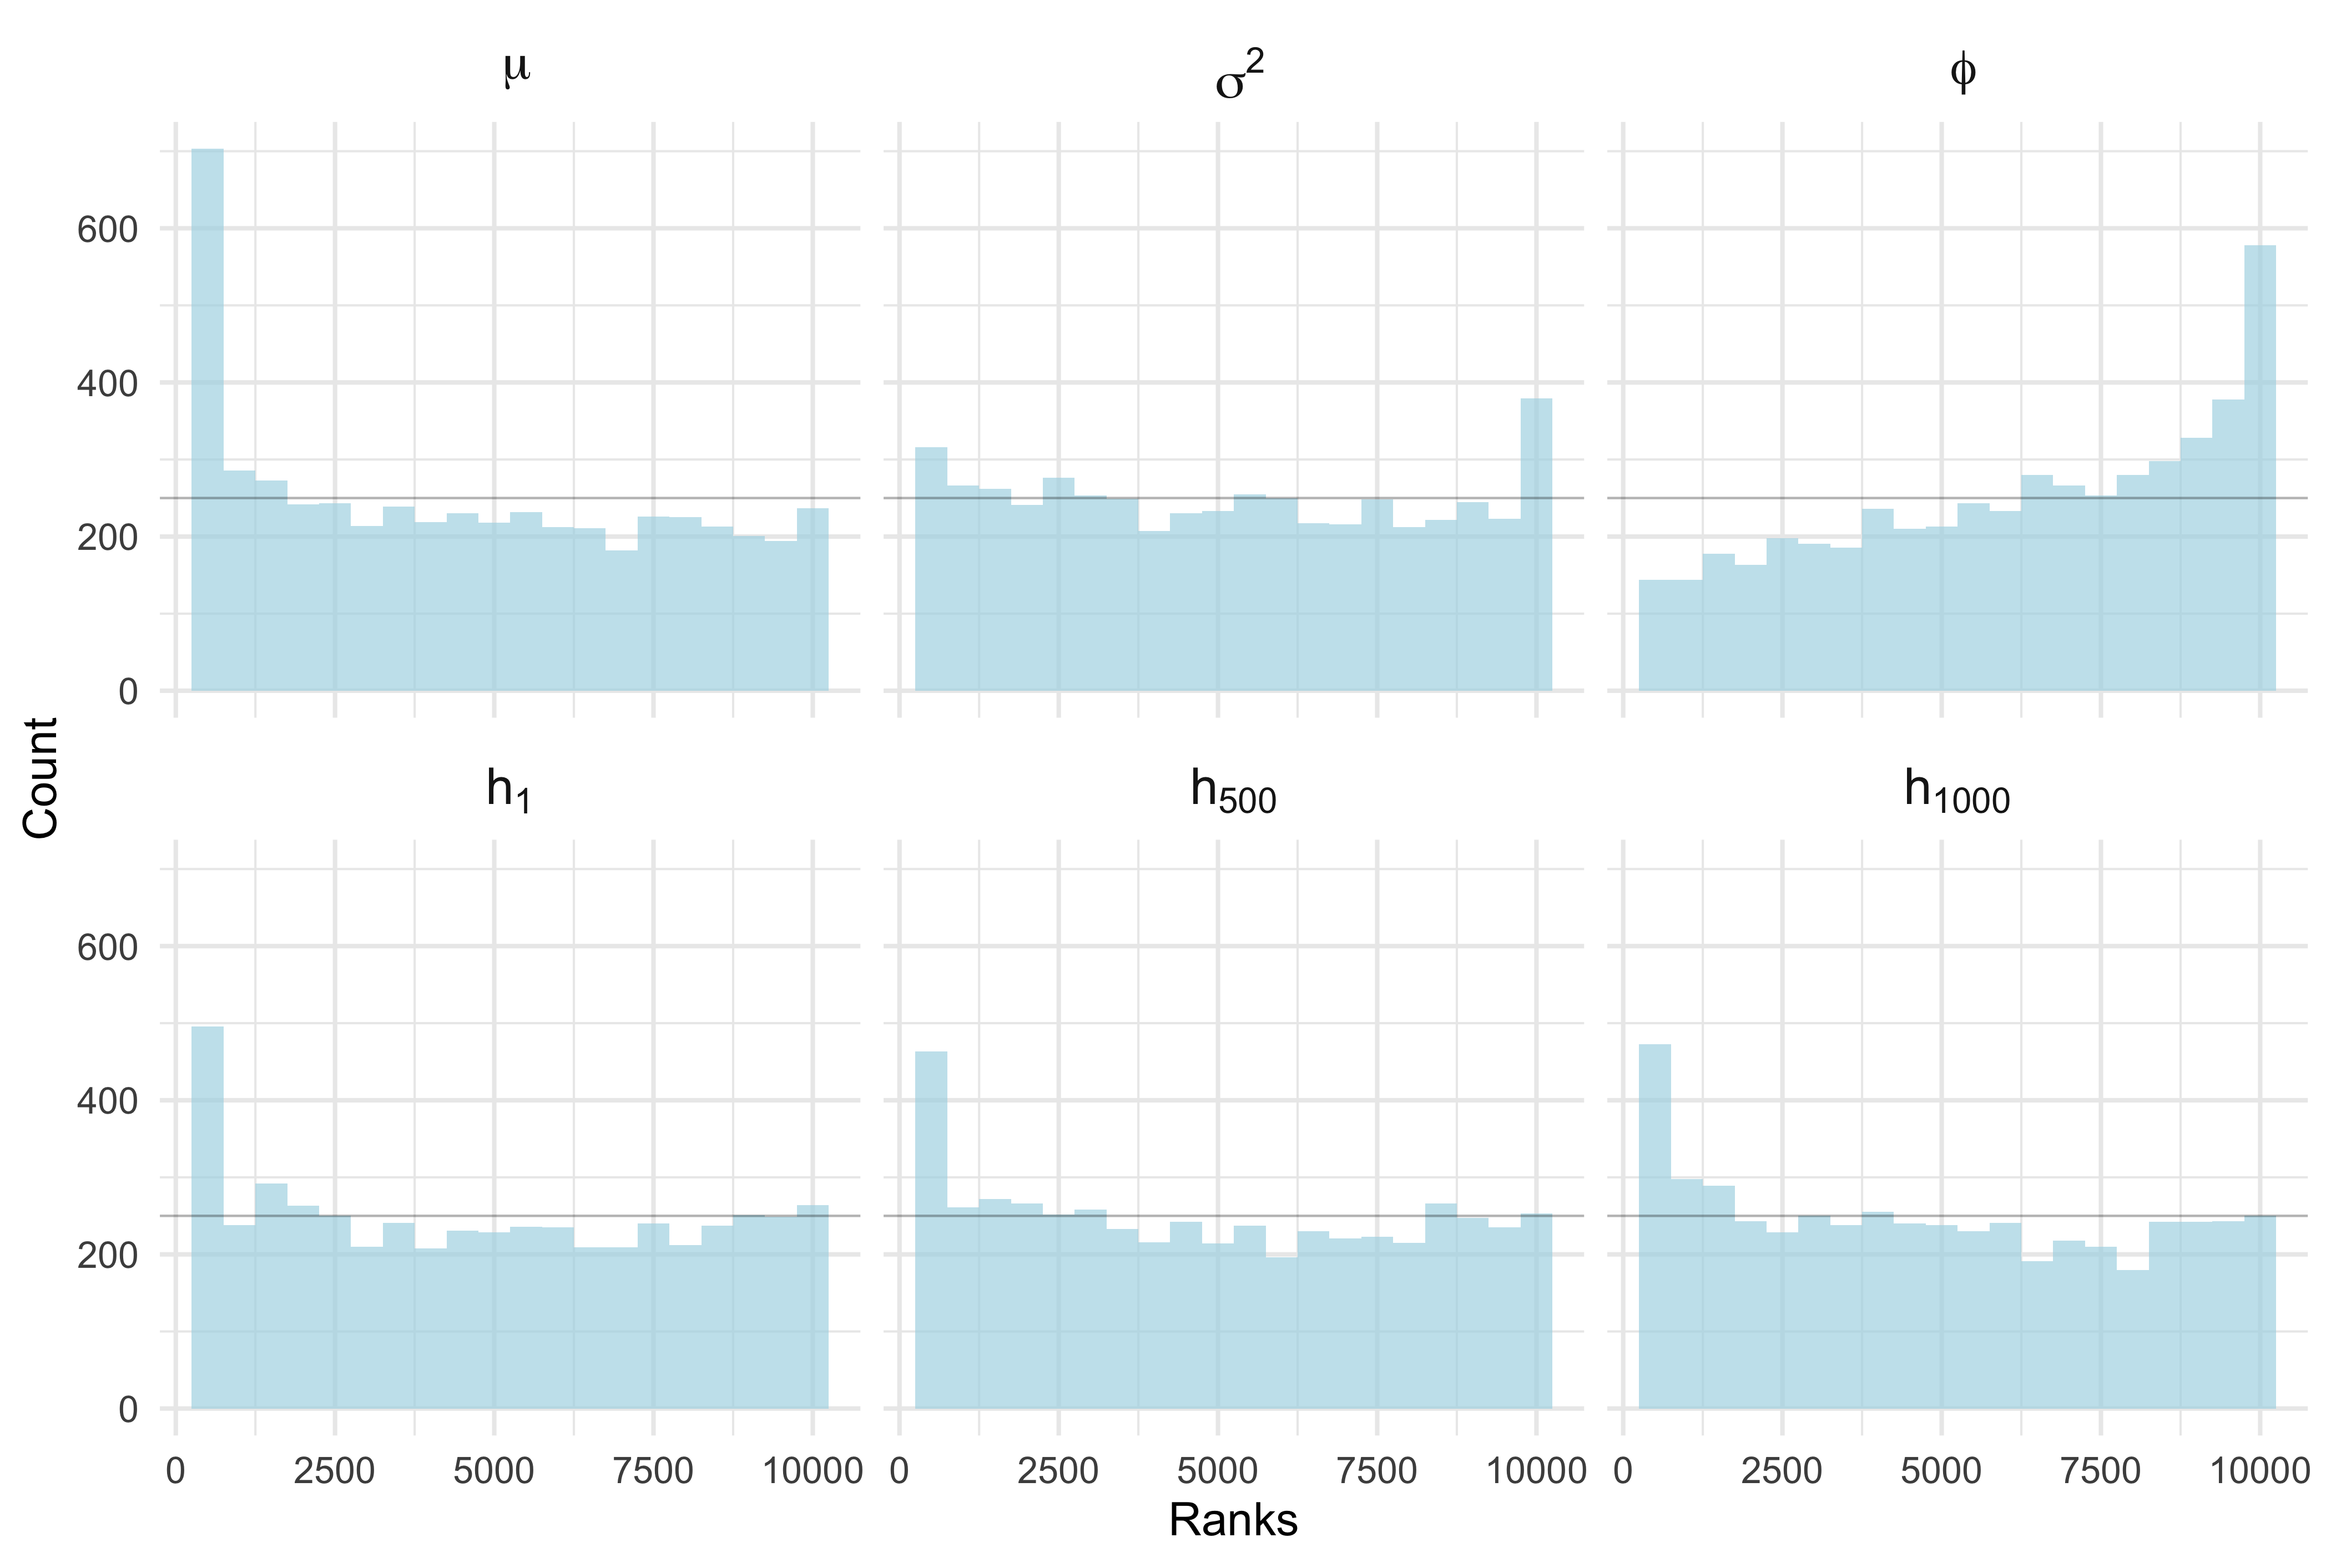
\includegraphics[scale=0.1]{results/weighted_ksc_cp_5k.png}
        \caption{5000 SBC iterations for re-weighted rank statistics from the Gaussian mixture approximation model. No major improvements are observed to the uniformity of rank statistics.}
        \label{fig:reweight5k}
    \end{figure}

    \subsection{Evaluating SBC for state variables}
    It is not practical to inspect the histograms of all parameters and states in the stochastic volatility model. Instead, the chi squared statistic is used to summarise the shape of the rank statistic distribution. This will be used to summarise the state variables only since the static parameters can be compared across simulations individually. 

    The state variable chi squared statistics for centered and re-parameterised HMC, centered KSC and centered importance weighted KSC are reported as histograms in Figure \ref{fig:allchisq} (using results from 5000 SBC iterations). Re-parameterised KSC is omitted as its poor SBC performance just adds noise to the results. A chi squared statistic of 0 implies the sample is exactly uniformly distributed. Any value away from 0 captures variation or deviations from uniformity. This provides a high level summary of the state variables - how close their rank statistics are to being uniformly distributed and their distance relative to the other algorithms and parameterisations. 
    
    The HMC results are relatively close to zero. Both KSC and the importance weighted ranks on the other hand are far from zero suggesting major deviations from uniformity. There is a large gap between the HMC and KSC chi squared statistics implying the distribution of state variable ranks are much less uniform for KSC relative to the HMC. Combined with the results in the previous section, there is a strong evidence that HMC outperforms KSC where it comes to calibration across all parameters and latent state variables.

    \begin{figure}[H]
        \centering
        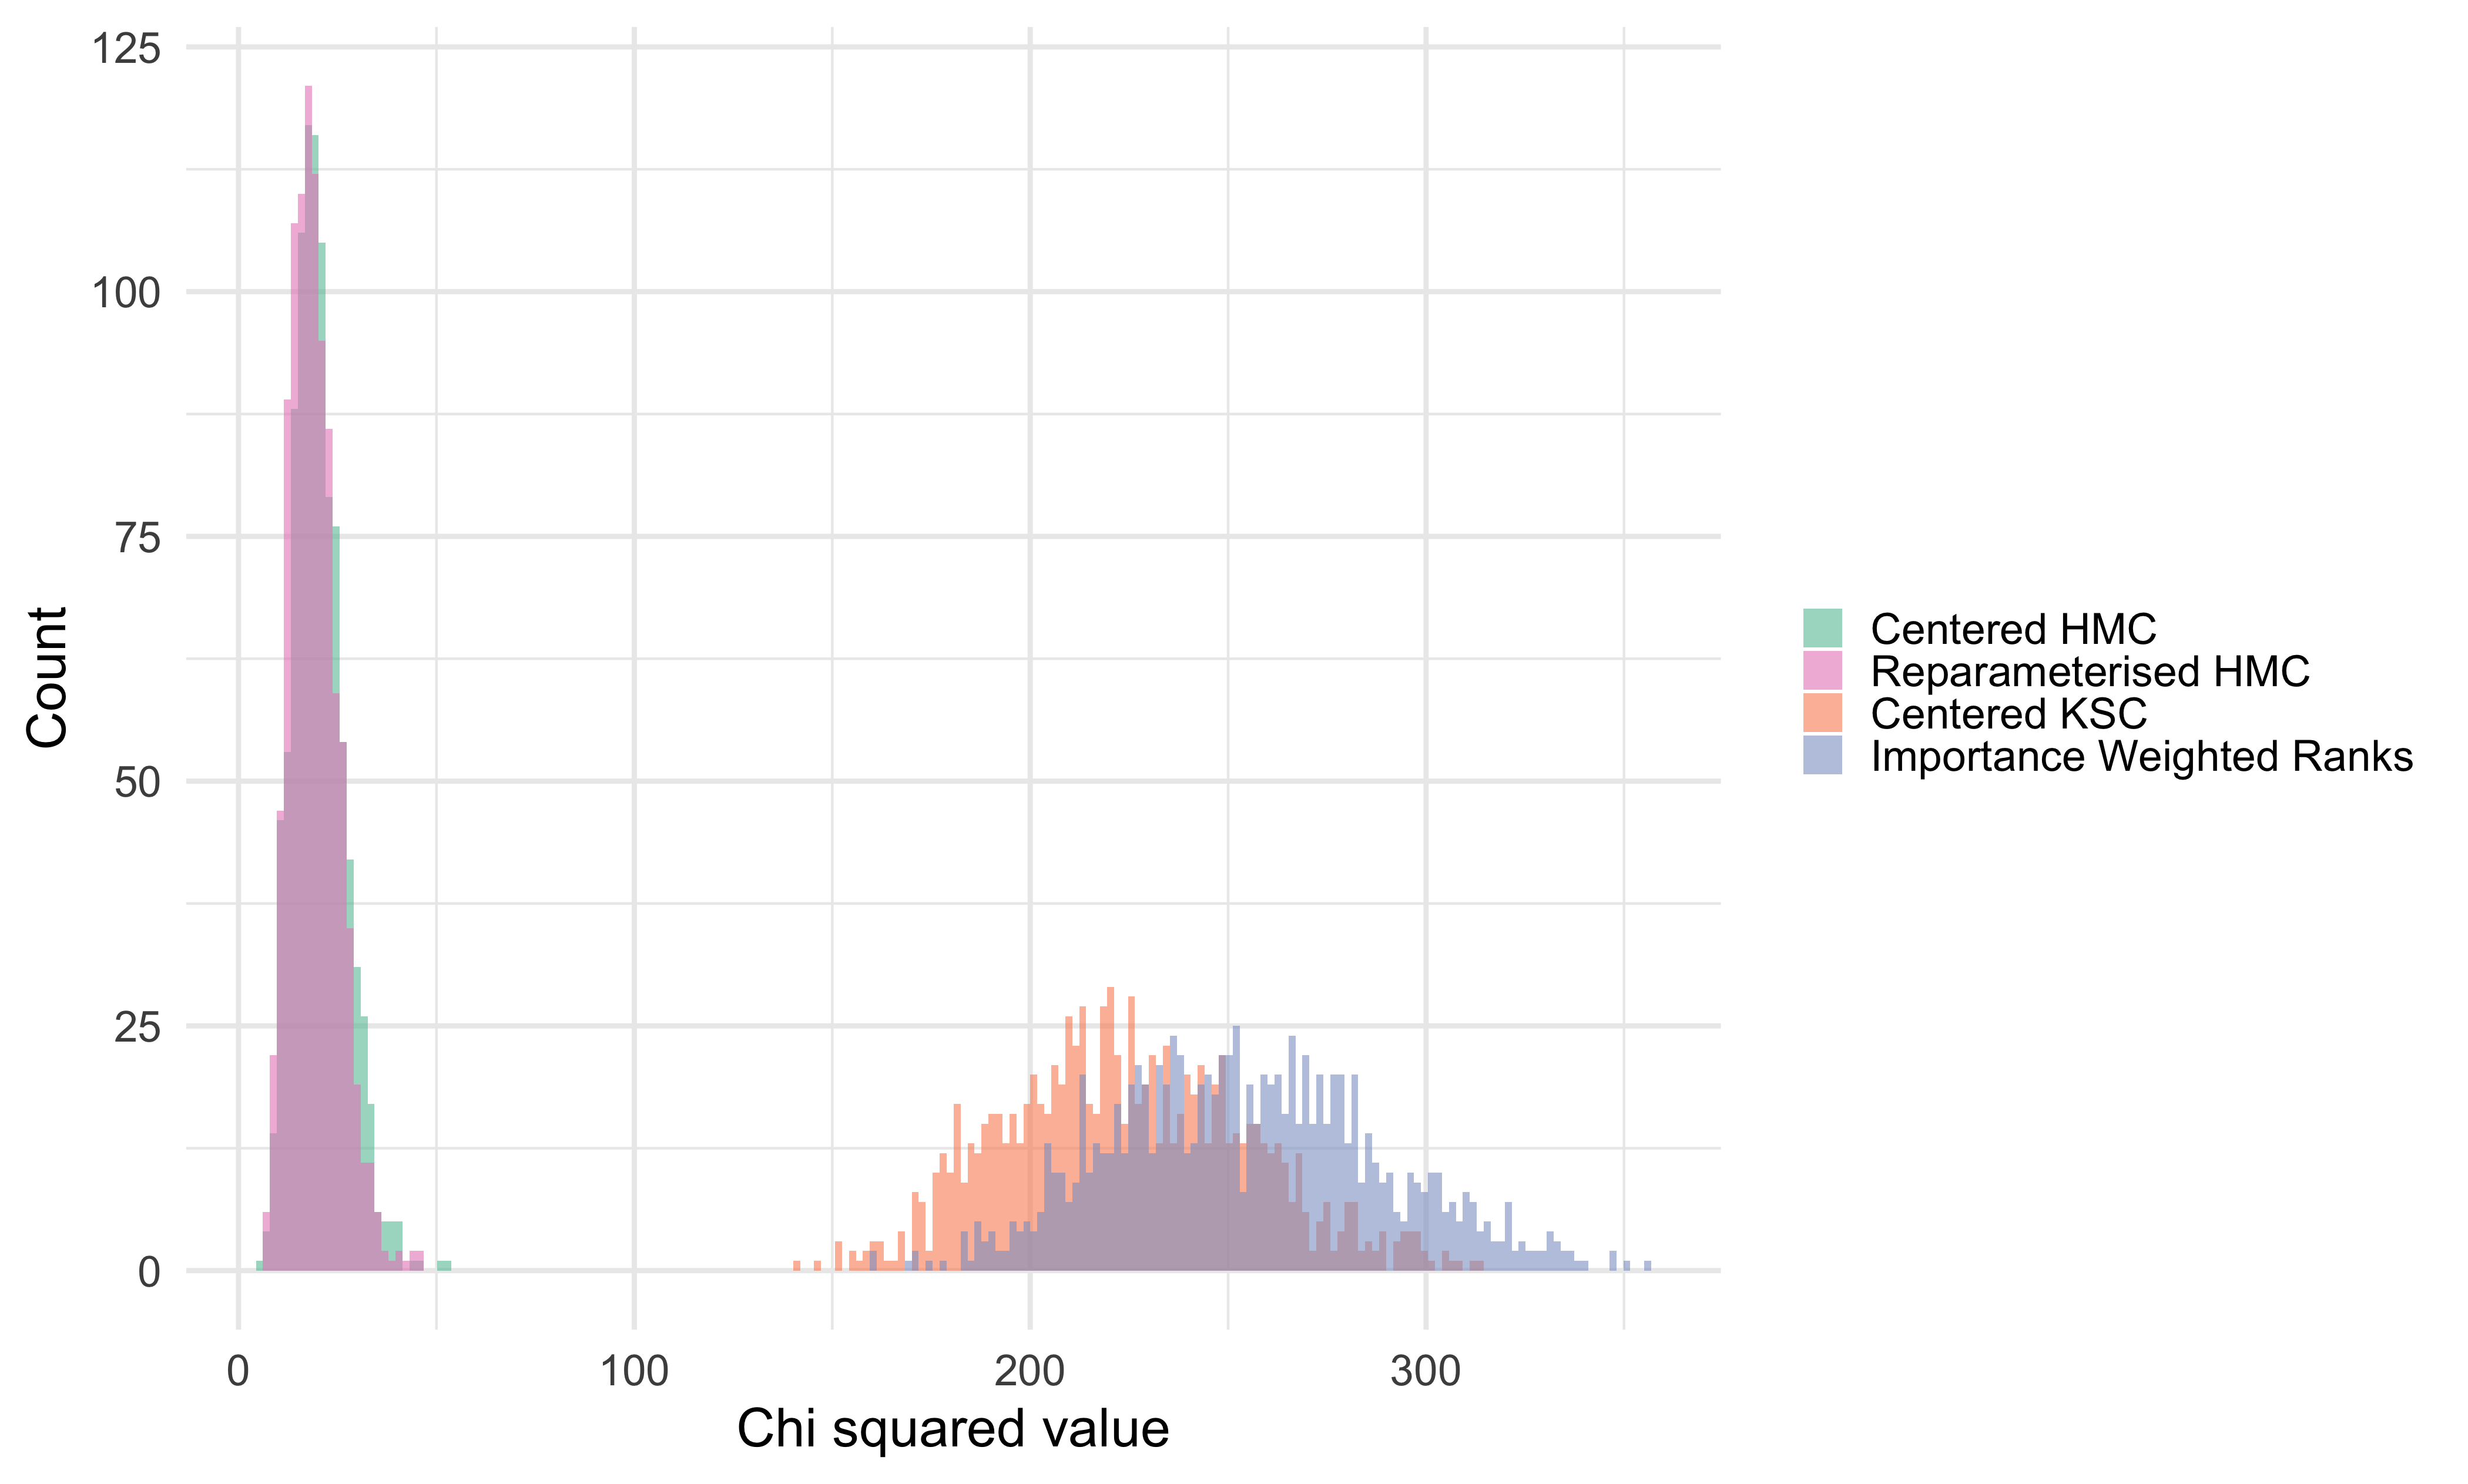
\includegraphics[scale=0.1]{results/dist_chisq_all.png}
        \caption{Distribution of chi squared statistics for latent state variables. Results from 5000 SBC iterations are used. Values closer to 0 are more consistent with a discrete uniform distribution. Both HMC simulations are much closer to zero than KSC. This suggests that the HMC algorithm overall produces more calibrated posterior estimates for the state variables}
        \label{fig:allchisq}
    \end{figure}

\section{Discussion}
Overall, Hamiltonian Monte Carlo applied on the re-parameterised model performs best based on calibration and efficiency results. Centered parameterisation using HMC performed moderately well but struggled to produce calibrated posterior estimates for $\sigma^2$ and $\phi$ as well as generate independent samples for these parameters. Gaussian mixture approximation struggled to return calibrated posterior estimates and efficient samples for both parameterisations. However, the centered parameterisation results for the Gaussian mixture model may improve if we increased the length of the Markov chain. This is discussed later in the limitations section. 

These results demonstrate that the performance of a MCMC algorithm is sensitive to the parameterisation of the model in the context of calibration and efficiency. Furthermore, the parameterisation of a model is conditional on the choice of MCMC algorithm. Evaluating the effectiveness of a modelling strategy (i.e choice of model, parameterisation and sampler) on simulated data gives a lot of a priori information about how the model will perform before it is fit on real data. Performing SBC may help isolate confounding factors if any problems occur. 

The priors chosen for this study came directly from \citet{kim1998stochastic}. The SBC results for the Gaussian mixture may improve if the priors were more informative - although this is only conjecture. Whether or not to use tighter priors depends on the modelling context and the problem at hand. If a model is expected to handle data generated by the priors, then un-calibrated results from SBC raises questions about the suitability about the model choice, MCMC or parameterisation. 

Other parameterisations of the stochastic volatility model are available as outlined in \citet{strickland2008parameterisation}, namely non centered in scale or both non centered in scale and location. The failure of non centered parameterisation in location for the Gaussian mixture model could be due to a variety of reasons. This may be due to a particular software implementation when it comes to the Kalman Filter and Simulation Smoother (where a specific software package was applied) that was not designed to handle the non centered parameterisations. Or perhaps this particular parameterisation does not suit the sampling strategy applied by KSC and another approach (e.g. HMC) might be more successful. Lots of different design and implementation details could be explored further. Pinpointing the reason why this model parameterisation failed as well as exploring other configurations and MCMC algorithms in this context is left to future research.

It is worth noting that there are many ways of comparing MCMC approaches. Other features that may be of interest is the speed in which a MCMC can converge onto the target distribution and generate samples for inference. However, speed is difficult to define and is subject to a variety of different factors such as hardware, operating system, and software versions. The purpose of this research is to compare algorithms based on calibration and efficiency. Additionally, this simulation study does not provide any advice on the appropriateness of the stochastic volatility model on real data. Whether the stochastic volatility model is appropriate for modelling a particular financial time series requires further study into the data generating process, domain expertise and a suite of other diagnostic checks. Examples of this are posterior predictive checking and out of sample predictive performance. Rather, the SBC approach gives insight into how well calibrated a sampling strategy is conditional on a known data generating process which is important in all applied contexts.  

% (other implementations exist as well but left for future research. lots of different design and implementation details could be explored. Let alone choice of algos.)

\section{Limitations}
A limitation to applying SBC in all modelling contexts is that it is computationally intensive. SBC requires fitting multiple models to get reliable estimates. In some cases, fitting just one model can take a long time, let alone multiple. Producing results for this research within a reasonable time-frame required use of a high performance cluster. Computing infrastructure may limit the opportunity for SBC to be performed. The choice of SBC iterations for this research was arbitrary and was used to demonstrate that noisy estimates could be reduced by increasing the number of iterations for calibrated models. A more principled approach to picking the number of SBC iterations could be explored in other research.

Diagnostic tools for evaluating SBC results and models with many parameters is an area for improvement. As discussed, inspecting many histograms for highly parameterised models is unrealistic. Other summary statistics and visualisations can be applied for a high level comparison, such as the chi squared statistics applied in this research. Furthermore, it is not always straightforward to understand why any any one parameter may produce poor calibration results, for example, an arbitrary latent state varaible. SBC may tell us some information about the miscalibration based on the histogram shape (e.g. underdispersed, overdispersed, or biased relative to the prior distribution), but understanding why this occurs may not be immediately clear. Although, diagnosing sampling problems with complicated posterior geometries speaks more generally to the difficulty of understanding complex models in the first place as opposed to a limitation of SBC.

Lastly, it is unclear what constitutes a fair comparison between algorithms when comparing SBC results. In particular, the number of post burn-in or warm-up samples differed between algorithms (999 post burn-in for HMC, 9999 for the bespoke algorithm). An argument could be made that the poor results for the bespoke KSC algorithm may be due to the chain not converging onto the target distribution. Indeed, the authors of this approach extended their Markov chain to 750,000 posterior draws (discarding the first 10,000 draws as burn-in). A fairer comparison may be to have roughly similar number of ESS for most of the estimated parameters, although this is difficult to get right with a large number of parameters and variables to estimate. Given how well Hamiltonian Monte Carlo performed with the re-parameterised model, any improvement to the Gaussian mixture model by increasing the length of the Markov chain would make calibration just as good, but not better due to the inefficiency of the sampler. 

\section{Conclusion}
This research evaluated and compared different MCMC algorithms for fitting stochastic volatility models. As our models and algorithms for estimating these models become more complicated, so does the need for principled ways of checking that they are returning correct posterior estimates. SBC provides a general simulation design to check whether a modelling strategy is producing calibrated results for generative models.

In the context of stochastic volatility, applying Hamiltonian Monte Carlo on a re-parameterised stochastic volatility model provided the most calibrated and efficient estimates when compared with KSC's bespoke MCMC method. This also outperformed the KSC model using importance sampling weights to correct for approximation error. Other parameterisations of the stochastic volatility model can be considered to see if it improves sampling performance based on these diagnostics. 

This study only considered a handful of potential algorithms, sampling strategies and parameterisations for stochastic volatility. Future research could use the same SBC design to compare and evaluate more complicated volatility models and MCMC algorithms. Overall, SBC is a valuable tool in model development and is a key part of a statistical workflow. 
 
\newpage

\bibliography{references}

\newpage

\section{Appendix A: Mixture Gaussian weights}

\begin{table}[H]
    \centering
    \begin{tabular}{lccc} 
          $\omega$ &$Pr(\omega = i)$&  $m_i$&  $\nu^2_i$\\ 
          1&0.00730  &  -10.12999&  5.79596\\ 
          2&0.10556  &   -3.97281 &  2.61369\\ 
          3&0.00002 &  -8.56686 &   5.17950\\ 
          4&0.04395 &  2.77786  &   0.16735 \\ 
          5&0.34001&   0.61942    &  0.64009\\ 
          6&0.24566 &  1.79518    &  0.34023 \\ 
          7&0.25750 &  -1.08819    &  1.26261\\ 
    \end{tabular} 
\end{table}

\newpage

\section{Appendix B: Sampling from mixture of Gaussian's}

\subsection*{Conjugate posterior distributions}

\textbf{Sampling} $\boldsymbol{\sigma_{\eta}^2}$

Inverse gamma conjugate posterior distribution:

$$
\sigma^2_{\eta} | y,h,\phi,\mu \sim IG \Bigl\{\frac{n+\sigma_r}{2}, \frac{0.05 + (h_1 - \mu)^2 (1 - \phi^2) + \sum_{t=1}^{n-1}((h_{t+1} - \mu) - \phi(h_t - \mu))^2}{2}\Bigr\}
$$

\textbf{Sampling}  $\boldsymbol{\mu}$

Gaussian conjugate posterior distribution:

$$
\mu | h,\phi,\sigma^2_{\eta}  \sim N(\hat{\mu}, \sigma^2_{\mu})
$$

Where

$$
\begin{aligned}
\hat{\mu} &= \sigma^2_{\mu} \Bigl\{\frac{(1-\phi^2)}{\sigma_{\eta}^2}h_1 +\frac{(1-\phi^2)}{\sigma_{\eta}^2} \sum_{t=1}^{n-1} (h_{t+1} - \phi h_t)\Bigr\} \\
\sigma^2_{\mu} &= \sigma^2_{\eta} \{(n-1)(1-\phi)^2 + (1-\phi^2)\}^{-1}
\end{aligned}
$$

\subsection*{Metropolis Hastings Step}
\textbf{Sampling}  $\boldsymbol{\phi}$

Metropolis Hastings accept/reject procedure:

1) Generate proposal $\phi^\ast$ from $N(\hat{\phi}, V_{\phi})$ where $\hat{\phi} = \frac{\sum_{t=1}^{n-1} (h_{t+1} - \mu)(h_t - \mu)}{\sum_{t=1}^{n-1} (h_t - \mu)^2}$ and $V_{\phi} = \sigma^2_{\eta} \{\sum_{t=1}^{n-1} (h_t - \mu)^2\}^{-1}$

2) Accept proposal as $\phi^{(i)}$ with probability $e^{\{g(\phi^\ast) - g(\phi^{(i-1)}\}}$ such that $g(\phi) = log (\pi (\phi)) - \frac {(h_t - \mu)^2 (1-\phi^2)}{2 \sigma_{\eta}^2} + \frac{1}{2} log (1-\phi^2)$

\subsection*{Sampling mixture density}

Rewrite mixture density with respect to a indicator variable $s_t$

$$
\begin{aligned}
&z_t | s_t = i \sim N(m_i - 1.2704, \nu^2) \\
&Pr(s_t = i) = q_i
\end{aligned}
$$

Sample $s_t$ from probability mass function: 

$$
\begin{aligned}
Pr(s_t = i | y_t^{\ast}, h_t) \propto q_i f_N(y_t^{\ast} | h_t + m_t - 1.2704, \nu^2)
\end{aligned}
$$

\newpage

\section{Appendix C: Hamiltonian Monte Carlo algorithm description}
Let $\theta$ be a target parameter and $\phi$ be the auxiliary momentum variable. The Hamiltonian is defined as:

$$
\begin{aligned}
H(\theta, \phi) \equiv - log \: \pi(\theta, \phi)
\end{aligned}
$$

This can be broken down into kinetic energy $K(\theta, \phi)$, the density over the auxiliary momentum, and potential energy $V(\theta)$, the density of the target posterior distribution.

$$
\begin{aligned}
H(\theta, \phi) &= - log \: \pi(\phi | \theta) - log \: \pi(\theta) \\ 
&\equiv  K(\theta, \phi) + V(\theta)
\end{aligned}
$$

 Starting with an initial draw of $\theta$ (user defined or randomly generated), the HMC iteration or proposal is determined by 3 steps.

1) Randomly sample a momentum value

$$
\begin{aligned}
\phi\sim Multinormal(0, M)
\end{aligned}
$$

Where M is some diagonal mass matrix (assuming independence between momentum variables).

2) Solve the set of Hamiltonian (differential) equations which generates a proposal $(\theta^{\ast}, \phi^{\ast})$

$$
\begin{aligned}
\frac{\partial \theta}{\partial t} &= \frac{\partial H}{\partial \phi} = \frac{\partial K}{\partial \phi} \\
\frac{\partial \phi}{\partial t} &= \frac{\partial H}{\partial \theta} = - \frac{\partial K}{\partial \theta} - \frac{\partial V}        {\partial \theta}
\end{aligned}
$$

Where $\frac{\partial V}{\partial \theta}$ is the gradient of the target posterior density. The solution to these differential equations is approximated using a Leapfrog integrator which gives a discrete approximate solution. The parameters which are tuned in this process are the number of steps $L$ and the size of the steps $\epsilon$. The Leapfrog algorithm performs a half step of $\phi$ and then a full step of the parameter $\theta$, and another half step of the momentum variable $\phi$ and repeats this $L$ times. The final step is the proposal $(\theta^{\ast}, \phi^{\ast})$.

$$
\begin{aligned}
\phi &\leftarrow \phi - \frac{\epsilon}{2} \frac{\partial V}{\partial \theta} \\
\theta &\leftarrow \theta + \epsilon M^{-1} \phi \\
\phi &\leftarrow \phi - \frac{\epsilon}{2} \frac{\partial V}{\partial \theta}
\end{aligned}
$$

3) Metrpolis Hastings Accept/Reject
Let $(\theta^{t-1}, \phi^{t-1})$ be the values before the Leapfrog integrator.

$$
\begin{aligned}
r = \frac{\pi(\theta^{\ast} | y) \pi(\phi^{\ast})}{\pi(\theta^{t-1} | y) \pi(\phi^{t-1})}
\end{aligned}
$$

With sampled value

$$
\theta^t = \begin{cases}
    \theta^{\ast},& \text{with probability } min(r,1)\\
    \theta^{t-1}, & \text{otherwise}
\end{cases}
$$

\section{Appendix D: Importance weighted rank statistics for re-parameterised model}

\begin{figure}[H]
    \centering
    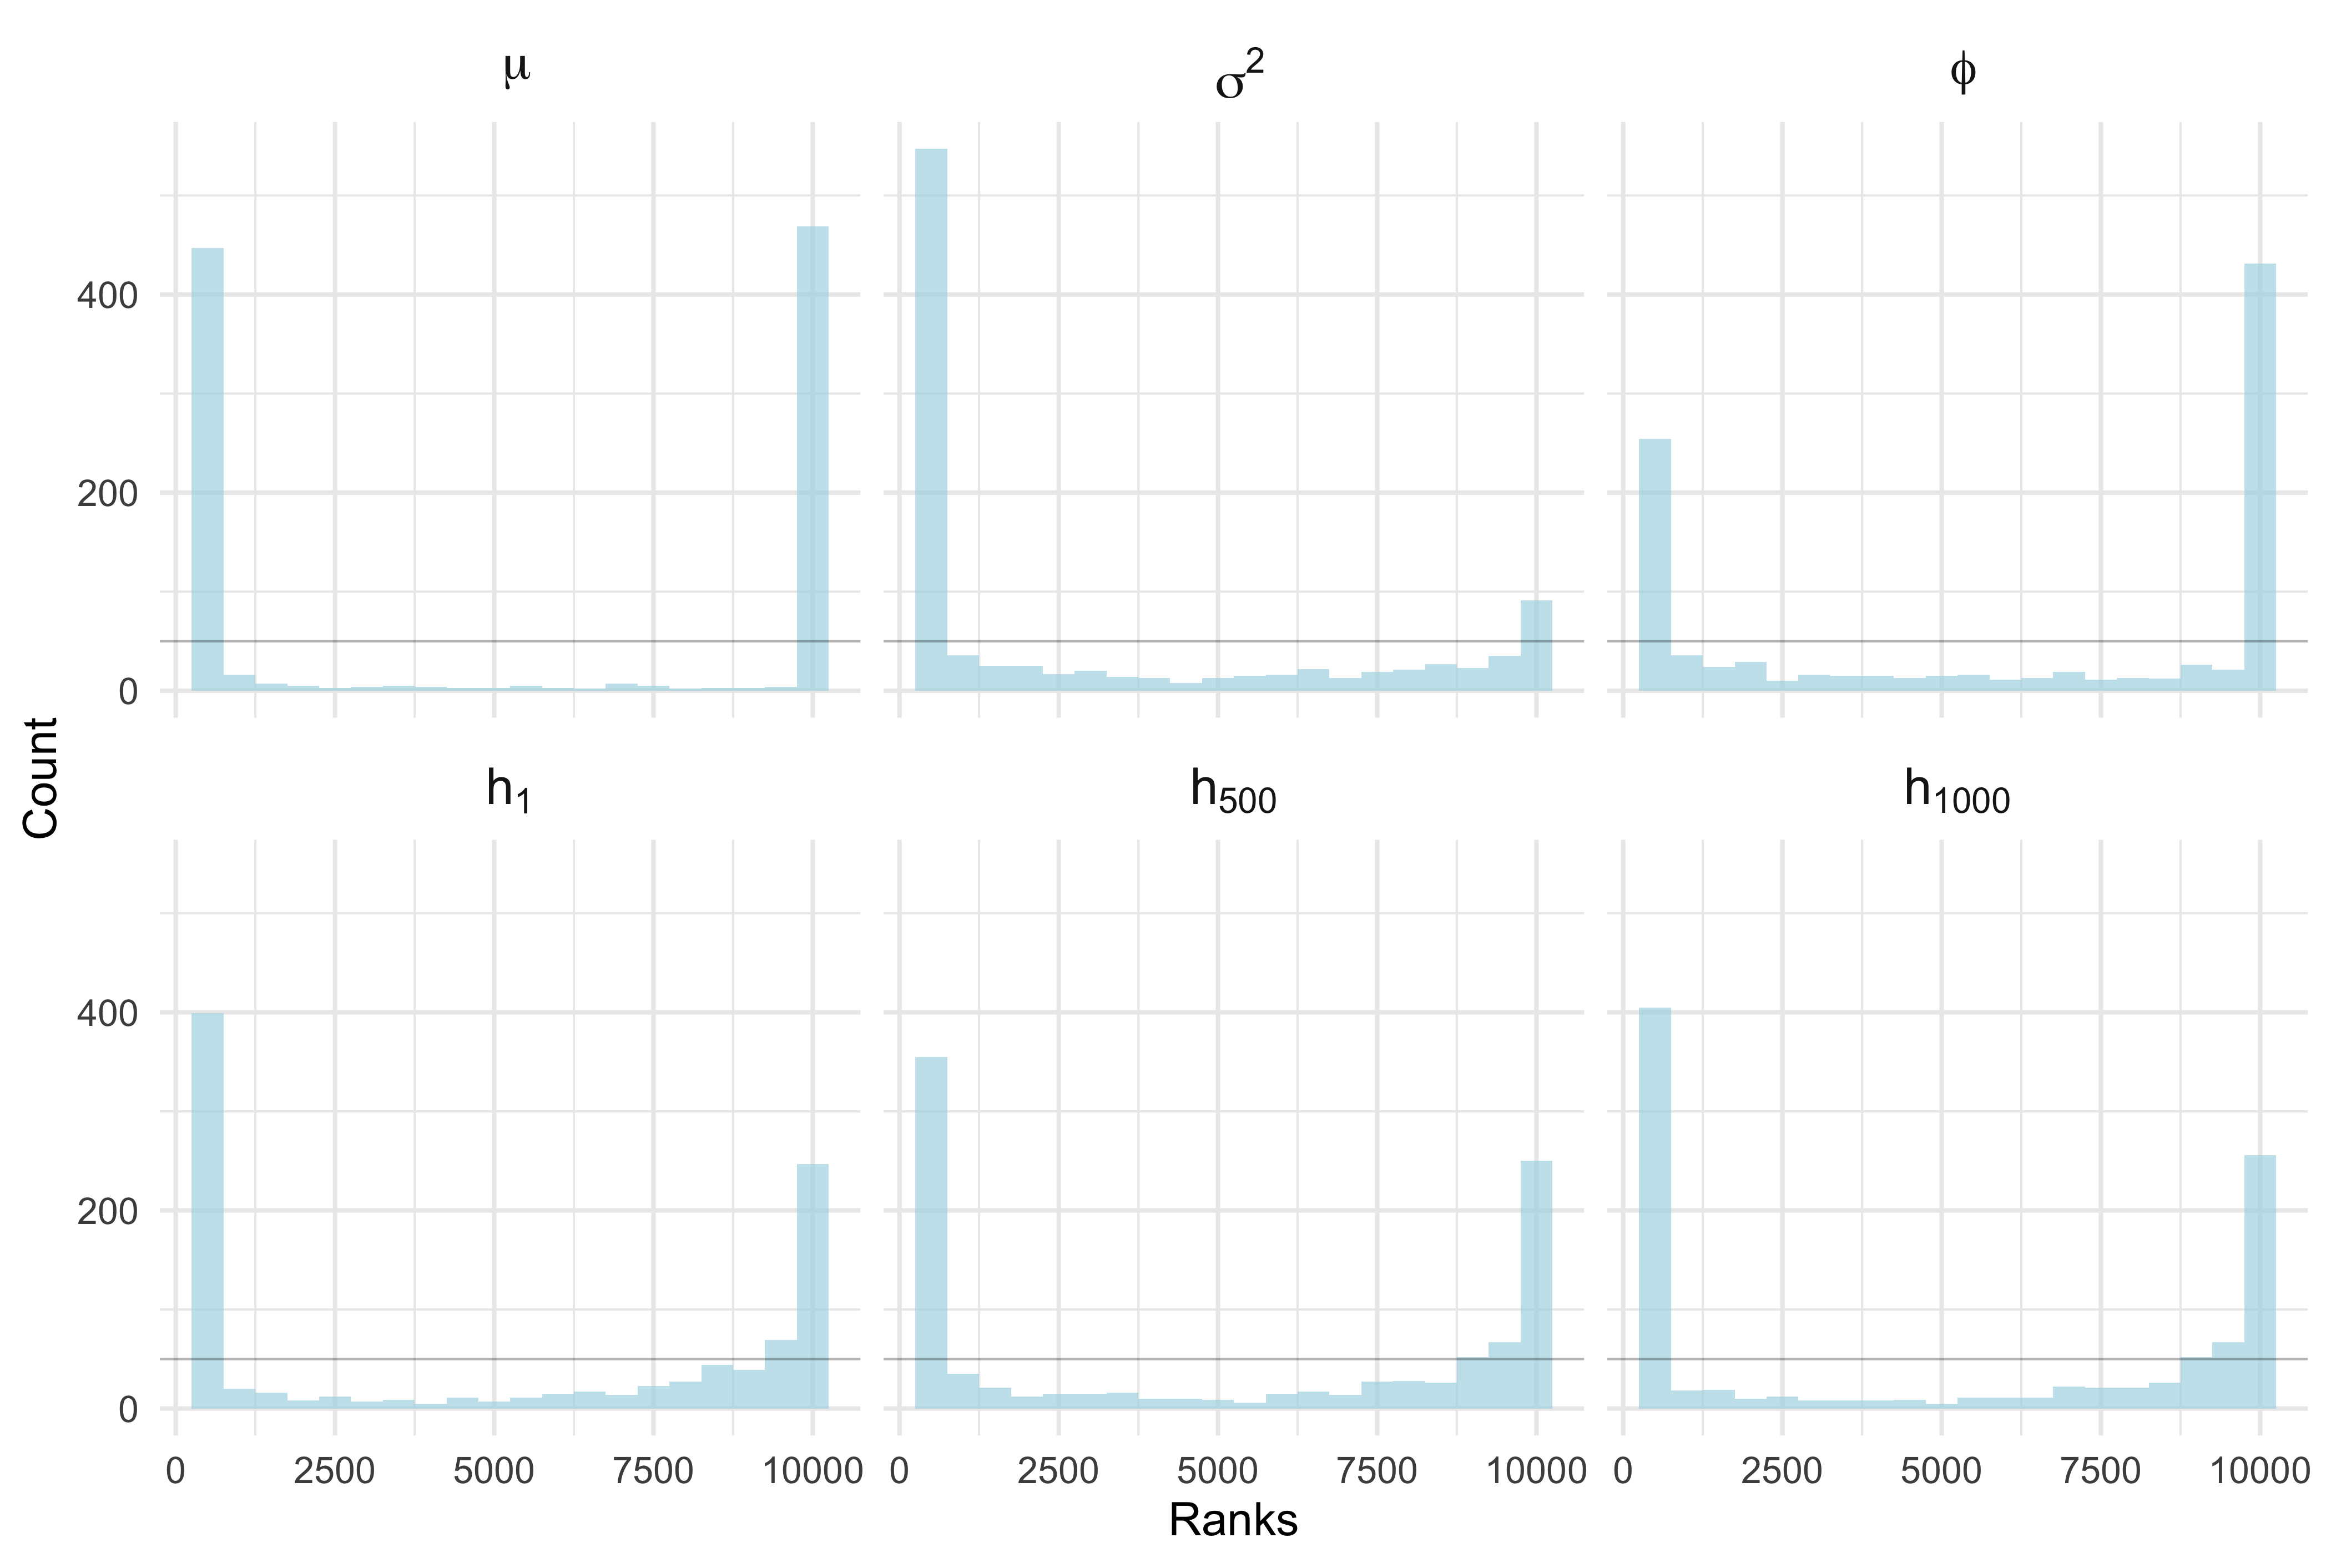
\includegraphics[scale=0.09]{results/weighted_ksc_ncp_1k.png}
    \caption{1000 SBC iterations for re-weighted rank statistics from the re-parameterised Gaussian mixture approximation model. The shape of the histogram is consistent with the unweighted rank statistics.}
    \label{fig:reweight1k}
\end{figure}

\begin{figure}[H]
    \centering
    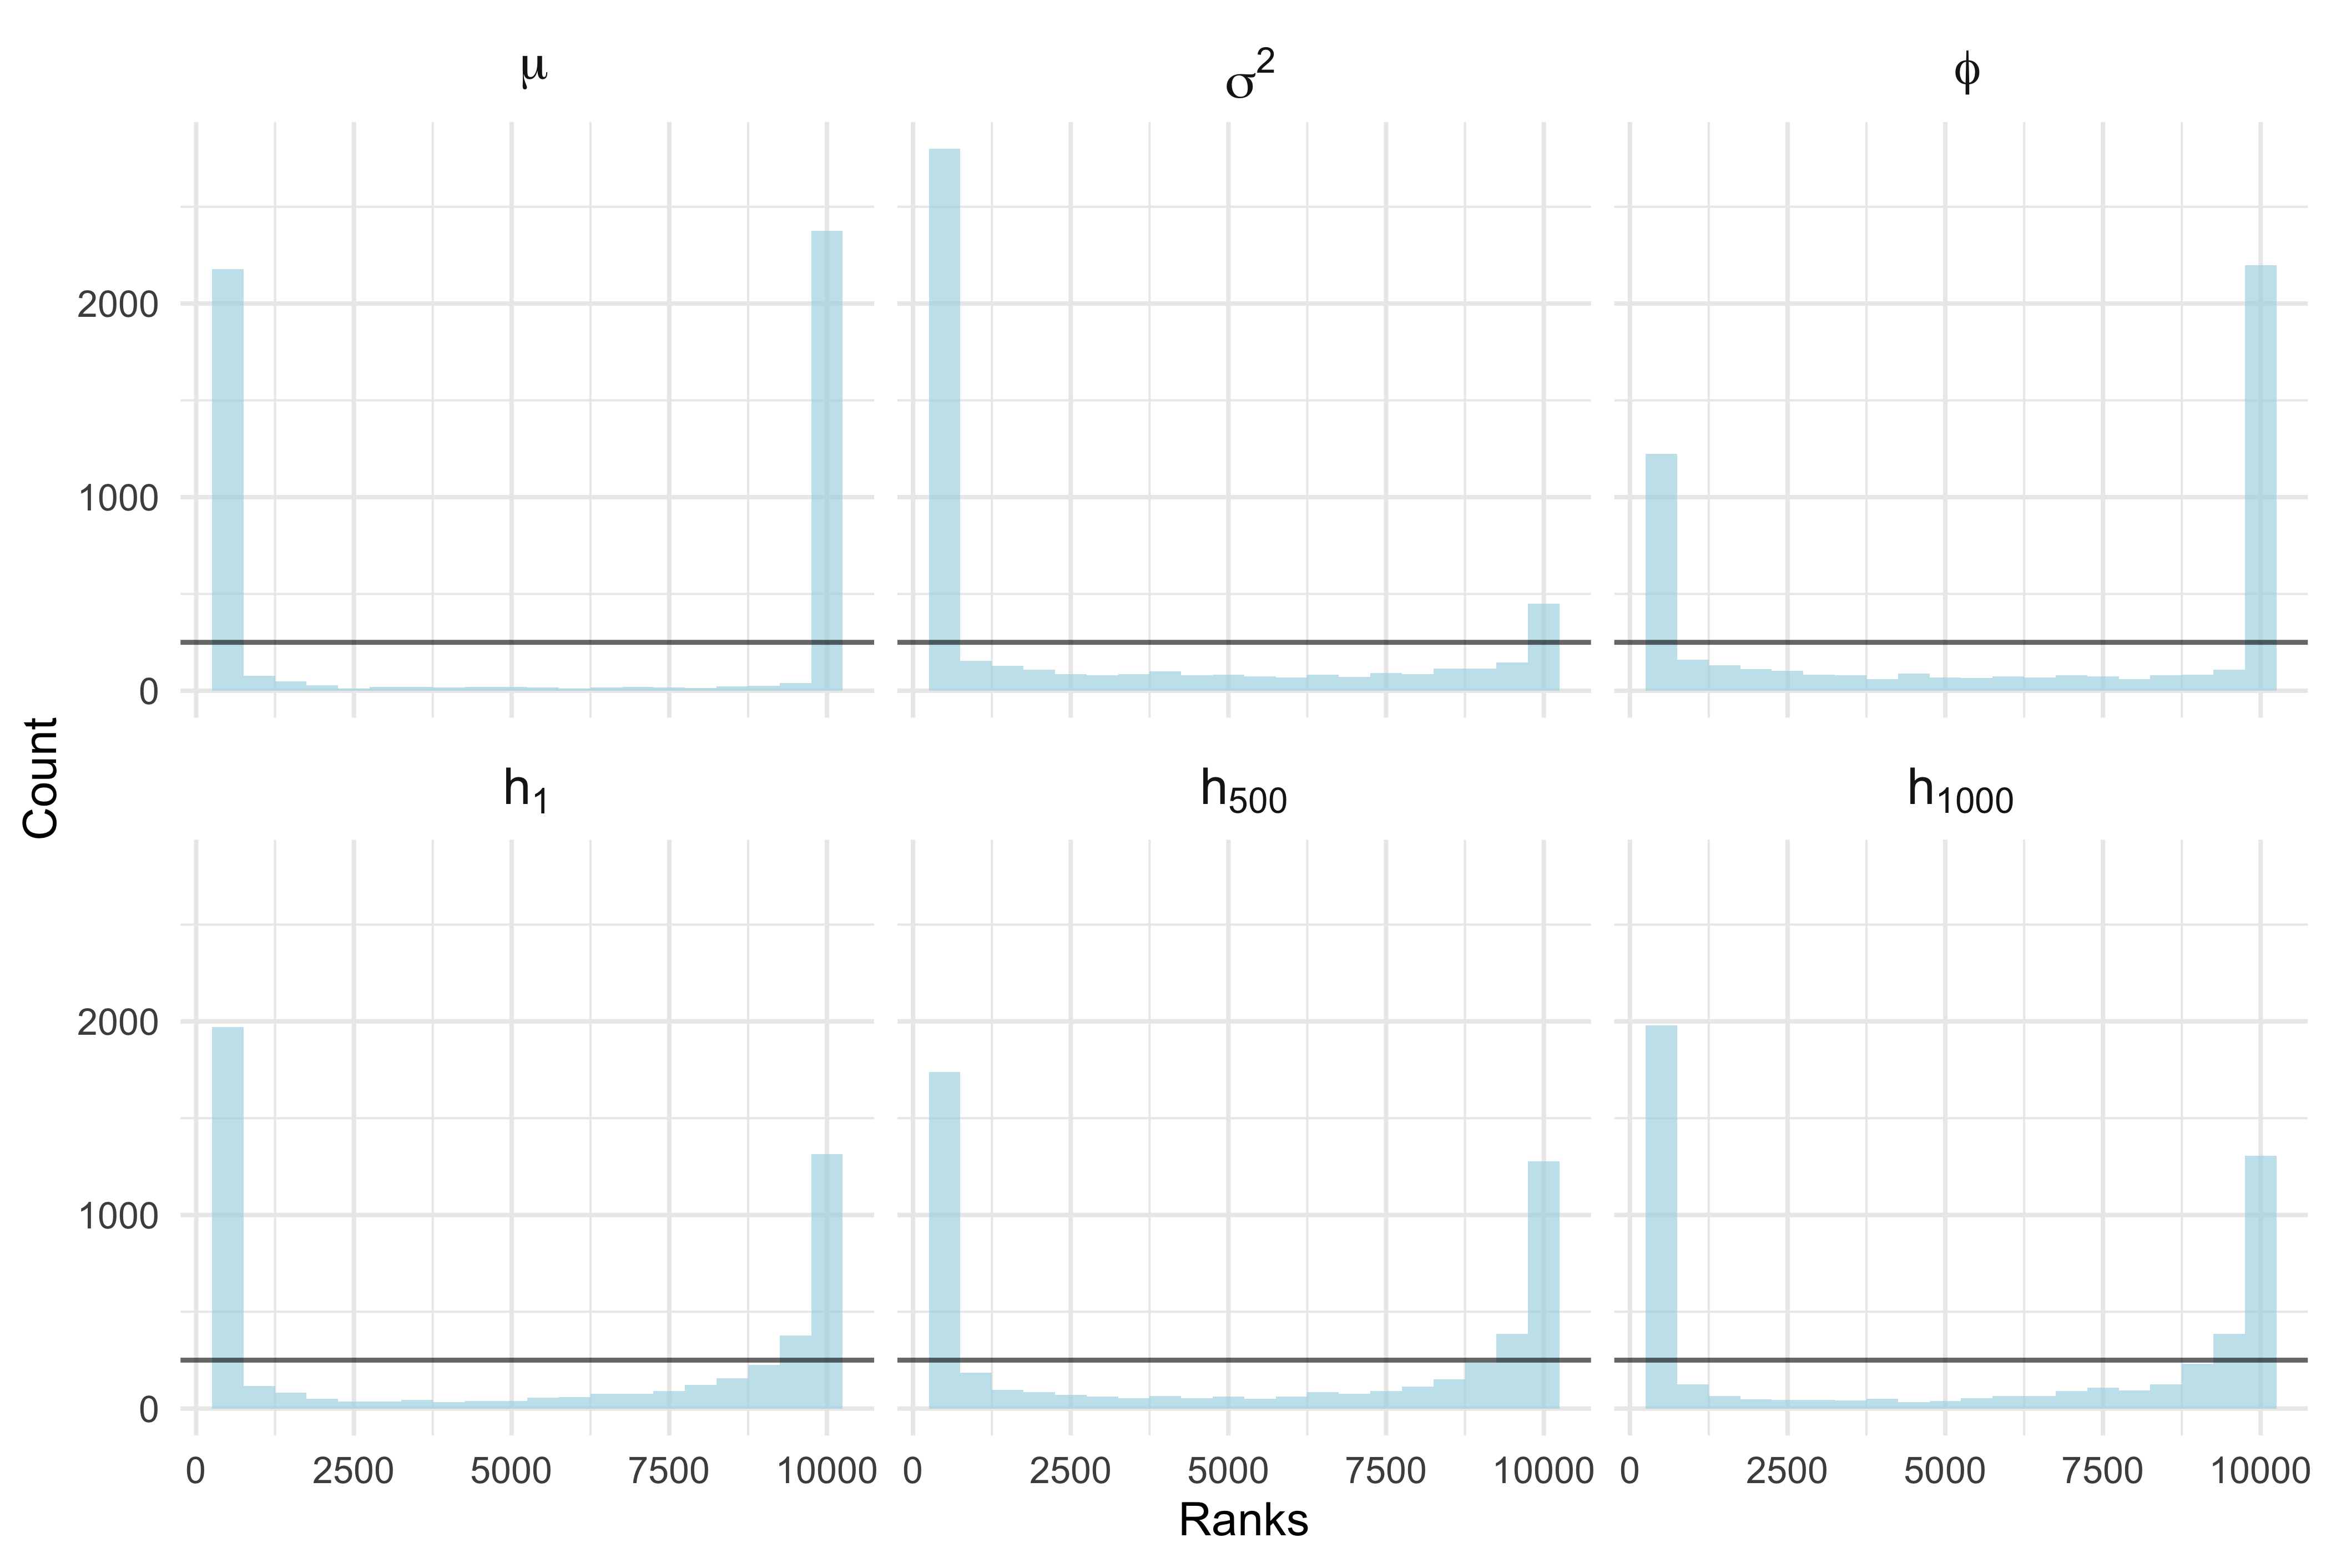
\includegraphics[scale=0.09]{results/weighted_ksc_ncp_5k.png}
    \caption{5000 SBC iterations for re-weighted rank statistics from the re-parameterised Gaussian mixture approximation model. No major improvements are observed to the uniformity of rank statistics.}
    \label{fig:reweight5k}
\end{figure}

\end{document}
